\chapter[Crossing countries: oddness in non-scalar Hurford Conditionals]{Crossing countries: oddness in non-scalar Hurford Conditionals\footnotemark}\label{chap:hurford-sentences}
\footnotetext{This Chapter builds on \citettoappear{HenotMortier2024a}, but develops a different (hopefully clearer and more principled) view on Hurford Conditionals. A number of similar intuitions will be exploited, including intuitions about granularity. I would like to thank the audiences and reviewers of the 2024 BerlinBrnoVienna Workshop, SuB29, and the 2024 Amsterdam Colloquium for relevant questions, datapoints and suggestions regarding this project and adjacent data. I want to give specials thanks to Amir, who first advised me to read \citet{Lewis1988} almost two years ago, and Viola, who very wisely advised me to take another look at it this Spring. }

This Chapter extends the empirical landscape introduced in Chapter \ref{chap:hurford-disj}, which was mainly interested in Hurford Disjunctions, of the form $p \vee p^+$ or $p^+ \vee p$, with $p^+ \vDash p$. This Chapter is an investigation of Hurford \textit{Conditionals} \citep{Mandelkern2018,Kalomoiros2024}, of the form \textit{If $p$ then $\neg p^+$} or \textit{If $\neg p^+$ then $p$}, with $p^+ \vDash p$. Such conditionals are related to Hurford Disjunctions by the \textit{or}-to-\textit{if} tautology; but (arguably) unlike their disjunctive counterparts, they exhibit a crisp asymmetry: variants in which the negated stronger proposition is in the antecedent (\textit{If $\neg p^+$ then $p$}) are degraded, while variants in which the negated stronger proposition is in the consequent (\textit{If $p$ then $\neg p^+$}), are fine. This Chapter explains this asymmetry, by building once again on the implicit QuD framework introduced in Chapter \ref{chap:accommodating-quds}, and by proposing a new constraint on Qtree derivation, dubbed \textsc{Incremental Q-Relevance}, building on \citeauthor{Lewis1988}'s and \citeauthor{Roberts2012}'s approaches to propositional \textsc{Relevance}. This will predict that the antecedent and consequent of Hurford Conditionals should be ordered in terms of their conveyed degree of granularity; and will be shown to successfully extend to variants of these sentences. More broadly, this Chapter suggests that Hurford Disjunctions and Conditionals, display different ``flavors of oddness''.




\section{Introducing Hurford Conditionals}

Let us start by reviewing familiar data. As discussed in Chapter \ref{chap:hurford-disj}, Hurford Disjunctions (henceforth \textbf{HD}s), exemplified in (\ref{ex6:hd}), feature contextually entailing disjuncts ($p^+ \vDash_c p$), and are generally odd regardless of the order of their disjuncts \citep{Hurford1974}.\footnote{When the two disjuncts are the same modulo scalar expressions (e.g. $\langle$\textit{some}, \textit{all}$\rangle$) HDs \textit{may} be rescued from infelicity \citenp{Gazdar1979}; \citenp{Singh2008b}; \citenp{Fox2018}; \citenp{HenotMortier2023} i.a.). Chapter \ref{chap:economy} provides an overview of the challenges raised by ``scalar'' Hurford Sentences, and proposes an account elaborating on the framework introduced here.}

\begin{exe}
	\ex \label{ex6:hd}
	\begin{xlist}
		\ex[\#] {SuB29 will take place in Noto or in Italy. \hfill $\pplus\vee \p$}\label{ex6:hd-sw}
		\ex[\#] {SuB29 will take place in Italy or in Noto. \hfill $\p \vee \neg \pplus$}\label{ex6:hd-ws}
	\end{xlist}
\end{exe}

\citet{Mandelkern2018} observed an intriguing, crisp contrast in so-called Hurford \textit{Conditionals} (henceforth \textbf{HC}s), exemplified in (\ref{ex6:hc}): (\ref{ex6:hc-sw}) is odd while (\ref{ex6:hc-ws}) is fine. As a side note, $\rightarrow$ will be used as a shorthand for \textit{if... then...}, throughout this Chapter (just like we did in Chapter \ref{chap:redundancy}), i.e. $\rightarrow$ will not imply that the conditionals under consideration are necessarily considered material.

\begin{exe}
	\ex \label{ex6:hc}
	\begin{xlist}
		\ex[\#] {If SuB29 will not take place in Noto, it will take place in Italy. \hfill $\neg \pplus\rightarrow \p$}\label{ex6:hc-sw}
		\ex[] {If SuB29 will take place in Italy, it will not take place in Noto. \hfill $\p \rightarrow \neg \pplus$}\label{ex6:hc-ws}
	\end{xlist}
\end{exe}

Why is the contrast in (\ref{ex6:hc}) intriguing? Granted conditionals are material, the HC in (\ref{ex6:hc-sw}) is equivalent to the HD in (\ref{ex6:hd-sw}), and can also be made structurally equivalent to it \textit{modulo} double-$\neg$ elimination. This is shown in (\ref{ex6:hd-hc-sw-derivation}). Therefore, it is perhaps unsurprising that (\ref{ex6:hc-sw}) appears degraded -- it can be understood as an HD ``in disguise''.

\begin{exe}
	\ex {(\ref{ex6:hc-sw}) $= \neg \pplus\rightarrow \p$ \\
		\phantom{(\ref{ex6:hc-sw})} $\equiv \neg(\neg \pplus)\vee \p$ \hfill (\textit{or}-to-\textit{if} tautology) \\
		\phantom{(\ref{ex6:hc-sw})} $\equiv \pplus\vee \p$ \hfill (double-$\neg$ elimination) \\
		\phantom{(\ref{ex6:hc-sw})} $=$ (\ref{ex6:hd-sw})}\label{ex6:hd-hc-sw-derivation}
\end{exe}

The surprise comes from (\ref{ex6:hc-ws}). Just like  (\ref{ex6:hc-sw}),  (\ref{ex6:hc-ws}) can be seen as a conditional of the form $\neg q^+ \rightarrow q$, with $q^+ \vDash q$, by taking $q^+$ to be the proposition that \textit{SuB29 will not take place in Italy} (so $q^+ = \neg p$), and $q$ to be the proposition that \textit{SuB29 will not take place in Noto} (so $q = \neg p^+$). Again, we have $q^+ \vDash q$, because $p^+ \vDash p$, and negation reverses entailments. This is all detailed in (\ref{ex6:hd-hc-ws-derivation}).

\begin{exe}
	\ex {(\ref{ex6:hc-ws}) $= \p \rightarrow \neg \pplus$\\ \phantom{(\ref{ex6:hc-ws})} $\equiv \neg (\neg \p) \rightarrow (\neg \pplus)$ \hfill (double-$\neg$ introduction)\\
		\phantom{(\ref{ex6:hc-ws})} $\equiv \neg \qplus\rightarrow \q$ \hfill ($\qplus := \neg\p$; $\q := \neg\pplus$; s.t. $\qplus \vDash \q$)\\
		\phantom{(\ref{ex6:hc-ws})} $\approxeq$ (\ref{ex6:hc-sw})}\label{ex6:hd-hc-ws-derivation}
\end{exe}

(\ref{ex6:hc-ws}) is thus structurally similar to (\ref{ex6:hc-sw}), though not logically equivalent to it. So, one could say (\ref{ex6:hc-sw}) and (\ref{ex6:hc-ws}) are ``isomorphic'', in the sense that they have same logical structure, and can be derived from each other \textit{via} a variable change preserving logical relations (see (\ref{ex6:iso}) for a formal definition). 
\begin{exe}
	\ex {\textsc{\textbf{Isomorphy}}. Let $X$ and $Y$ be two LFs. $X$ and $Y$ are isomorphic ($X \approxeq Y$) iff there is a substitution operation $\mathcal{S}$ targeting atomic propositions and preserving the logical relations between the elements in its domain ($aRb \iff \mathcal{S}(a)R\mathcal{S}(b)$, where $R$ denotes entailment, contradiction, or independence) s.t. $X$ and $\mathcal{S}(Y)$ have same parse.}\label{ex6:iso}
\end{exe}


This isomorphy between the infelicitous HC (\ref{ex6:hc-sw}) and the felicitous HC (\ref{ex6:hc-ws}) is problematic, because if (\ref{ex6:hc-sw}) is indeed an HD ``in disguise'', then so should (\ref{ex6:hc-ws}). Yet, this variant is felicitous. It appears that oddness in HCs is ``asymmetric''; descriptively,  the weaker item must be the antecedent, while the negated stronger item must be the consequent.\\


\citet{Kalomoiros2024} proposed the first solution to both the HDs (\ref{ex6:hd}) and  the HCs (\ref{ex6:hc}) (as well as other related datapoints). The approach was based on the idea that overt negation has a special status when it comes to evaluating if a sentence is redundant.

This Chapter argues for an alternative view, building on the idea that the questions evoked by an assertion must match the degree of granularity is conveys. The source of pragmatic oddness in HCs will then be tied to ``granularity'' violations, operationalized in terms of an incremental \textsc{Relevance} constraint. Roughly, this constraint will state that, whenever the question evoked by an assertion gets ``restricted'' to a certain domain of the Context Set, the domain must be \textsc{Relevant} to the question in a relatively standard sense, blending aspects of \citeauthor{Lewis1988}'s and \citeauthor{Roberts2012}'s view on \textsc{Relevance}. The directionality of this constraint will be directly tied to the computation of conditional Qtrees, which Chapter \ref{chap:accommodating-quds} defined as a kind of question-restriction.

According to this constraint, the HC in (\ref{ex6:hc-sw}) will be deemed deviant, essentially because its antecedent (\textit{not Noto}) does not rule out any cell from any question evoked by its consequent (\textit{Italy}). This is sketched in Figure \ref{tab:not-noto-italy-wh-rel1}.

\begin{figure}[H]
	\centering
	\begin{subfigure}[t]{.47\linewidth}
		\centering
		\begin{tabular}{llll|}
			\hline
			\multicolumn{2}{|l|}{Italy} & \multicolumn{1}{l|}{France} & ... \\ \hline
			\multicolumn{1}{l|}{}   & \multicolumn{3}{l|}{\cellcolor{orange!20!white}not Noto}         \\ \cline{2-4} 
		\end{tabular}
		\caption[]{(\ref{ex6:hc-sw})'s consequent is not \textsc{Relevant} to the ``\textit{wh}''-partition evoked by (\ref{ex6:hc-sw})'s antecedent.}\label{tab:not-noto-italy-wh-rel1}
	\end{subfigure}
	\hfill
	\begin{subfigure}[t]{.47\linewidth}
		\centering
		\begin{tabular}{llll|}
			\hline
			\multicolumn{2}{|l|}{Italy} & \multicolumn{2}{l|}{not Italy} \\ \hline
			\multicolumn{1}{l|}{}   & \multicolumn{3}{l|}{\cellcolor{orange!20!white}not Noto}      \\ \cline{2-4} 
		\end{tabular}
		\caption[]{(\ref{ex6:hc-sw})'s consequent is not \textsc{Relevant} to the ``polar''-partition evoked by (\ref{ex6:hc-sw})'s antecedent.}\label{tab:not-noto-italy-polar-rel1}
	\end{subfigure}
	\caption[]{How (\ref{ex6:hc-sw})'s antecedent interacts with (\ref{ex6:hc-sw})'s consequent's evoked questions.}
\end{figure}

The HC in (\ref{ex6:hc-ws}) on the other hand, will be predicted to be fine, because its antecedent (\textit{Italy}), interacts with the by-city partition evoked by its consequent (\textit{not Noto}) in the following way: first, it rules out some cells -- namely, all non-Italian city-cells -- and second, it rules in some cells -- namely, all Italian cities. This is sketched in Figure \ref{tab:italy-not-noto-wh-rel1}. 

\begin{figure}[H]
	\centering
	\begin{subfigure}[t]{.47\linewidth}
		\centering
		\begin{tabular}{|lll|ll}
			\hline
			\multicolumn{1}{|l|}{Noto} & \multicolumn{1}{l|}{Rome} & ... & \multicolumn{1}{l|}{Paris} & \multicolumn{1}{l|}{...} \\ \hline
			\multicolumn{3}{|l|}{\cellcolor{blue!20!white}Italy}                             & \multicolumn{2}{l}{}                                  \\ \cline{1-3}
		\end{tabular}
		\caption[]{(\ref{ex6:hc-ws})'s antecedent is \textsc{Relevant} to the ``\textit{wh}''-partition evoked by (\ref{ex6:hc-ws})'s consequent.}\label{tab:italy-not-noto-wh-rel1}
	\end{subfigure}
	\hfill
	\begin{subfigure}[t]{.47\linewidth}
		\centering
		\begin{tabular}{|lllll}
			\hline
			\multicolumn{1}{|l|}{Noto} & \multicolumn{4}{l|}{not Noto} \\ \hline
			\multicolumn{3}{|l|}{\cellcolor{blue!20!white}~~~Italy~~~}                &       &       \\ \cline{1-3}
		\end{tabular}
		\caption[]{(\ref{ex6:hc-ws})'s antecedent is not \textsc{Relevant} to the ``polar''-partition evoked by (\ref{ex6:hc-ws})'s consequent.}\label{tab:italy-not-noto-polar-rel1}
	\end{subfigure}
	\caption[]{How (\ref{ex6:hc-ws})'s antecedent interacts with (\ref{ex6:hc-ws})'s consequent's evoked questions.}
\end{figure}

The contrast between the two HCs will therefore arise from an interaction between our novel \textsc{Relevance} constraint, and the maximal level of granularity evoked by propositions, meaning, how fine-grained the leaves of their Qtrees can be.\\



This Chapter is structured as follows. Section \ref{sec6:prev-approaches} provides an overview of \citeauthor{Kalomoiros2024}'s approach to HCs, and outlines some of its limitations. Section \ref{sec6:machinery} uses the machinery introduced in Chapter \ref{chap:accommodating-quds} to derive questions evoked by HCs. Section \ref{sec6:relevance} motivates and defines \textsc{Incremental Q-Relevance} on LF-QuD pairs and shows how this constraint captures the HCs in (\ref{ex6:hd}) and (\ref{ex6:hc}). Section \ref{sec6:chc} explores variants of HCs and shows how \textsc{Incremental Q-Relevance} captures them. Section \ref{sec6:ccl} concludes and outlines remaining issues and questions.


\section{Existing account}\label{sec6:prev-approaches}

\citet{Mandelkern2018} show that HCs are problematic for virtually all accounts of HDs and their variants proposed before \citet{Kalomoiros2024}. Therefore, we will not review these approaches here, and directly jump to  \citeauthor{Kalomoiros2024}'s recent proposal.



\subsection{Super-Redundancy}
%HDs feel redundant; while HCs sound locally irrelevant.
%Talk about repairs: the fact the repairs are differnt suggets the violation stems from a different source.
\citeauthor{Kalomoiros2024}' \textsc{Super-Redundancy}, repeated in (\ref{ex4:sr}) from Chapter \ref{chap:redundancy}, states that a sentence $S$ is super-redundant if it features a binary operation taking a constituent $C$ as argument, and moreover there is no way of strengthening $C$ to $C^+$ that would make the resulting sentence $S^+$ non-redundant (i.e., non-equivalent to its counterpart where $C^+$ got deleted).

\begin{exe}
	\exr{ex4:sr} {\textsc{\textbf{Super-Redundancy}} \citep{Kalomoiros2024}. A sentence $S$ is infelicitous if it contains $C \ast C'$ or $C' \ast C$, with $\ast$ a binary operation, s.t. $(S)^-_C$ is defined and for all $D$, $(S)^-_C \equiv S_{Str(C, D)}$. In this definition:
		\begin{itemize}
			\item $(S)^-_C$ refers to $S$ where $C$ got deleted;
			\item  $Str(C, D)$ refers to a strengthening of $C$ with $D$, defined inductively and whose key property is that it commutes with negation ($Str(\neg\alpha, D) = \neg (Str(\alpha, D))$), as well as with binary operators ($Str(O(\alpha, \beta), D) = O(Str(\alpha, D), Str(\beta, D))$);
			\item $S_{Str(C, D)}$ refers to $S$ where $C$ is replaced by $Str(C, D)$.
	\end{itemize}}
\end{exe}

%HDs feel redundant; while HCs sound locally irrelevant.
%Talk about repairs: the fact the repairs are differnt suggets the violation stems from a different source.

As already shown in Chapter \ref{chap:hurford-disj}, this constraint can capture HDs (\ref{ex6:hd}). The proof, adapted from \citet{Kalomoiros2024}, is repeated in (\ref{ex5:hd-sr}).

\begin{exe}
	\exr{ex5:hd-sr} {HDs are Super Redundant (SR).\\
		We show (\ref{ex5:hd-sw})=$\pplus\vee\p$ and (\ref{ex5:hd-ws})=$\p\vee\pplus$ are SR.\\
		In either case, take C = \pplus.\\
		We then have (\ref{ex5:hd-sw})$^-_C$ = (\ref{ex5:hd-ws})$^-_C$ = $\p$\\
		$\forall D. \ (\textref{ex5:hd-sw})_{Str(C, D)} = (\textref{ex5:hd-ws})_{Str(C, D)} =  (\pplus \wedge D) \vee \p$\\
		\phantom{$\forall D. \ (\textref{ex5:hd-sw})_{Str(C, D)} = (\textref{ex5:hd-ws})_{Str(C, D)}$} $\equiv (\pplus \vee \p) \wedge (D \vee \p)$\\
		\phantom{$\forall D. \ (\textref{ex5:hd-sw})_{Str(C, D)} = (\textref{ex5:hd-ws})_{Str(C, D)}$} $\equiv \p \wedge (D \vee \p)$\\
		\phantom{$\forall D. \ (\textref{ex5:hd-sw})_{Str(C, D)} = (\textref{ex5:hd-ws})_{Str(C, D)}$} $\equiv (\p \wedge D) \vee \p$\\
		\phantom{$\forall D. \ (\textref{ex5:hd-sw})_{Str(C, D)} = (\textref{ex5:hd-ws})_{Str(C, D)}$} $\equiv \p = (\textref{ex5:hd-sw})^-_C = (\textref{ex5:hd-ws})^-_C$ 
	}
\end{exe}

More interestingly perhaps, (\ref{ex4:sr}) also captures HCs, whether conditionals are assumed to be material, or strict. The proofs assuming material conditionals, are given in (\ref{ex6:hc-sw-sr}) for (\ref{ex6:hc-sw}) and (\ref{ex6:hc-ws-sr}) for (\ref{ex6:hc-ws}). In both cases, it is crucial that the local strengthening of $C=p^+$ be conjunctive \textit{under} negation (and thus, disjunctive after applying De Morgan's law). In (\ref{ex6:hc-sw-sr}), this allows to remove $p^+$ from the chain of logical equivalences, and eventually derive Super-Redundancy. In the second part of (\ref{ex6:hc-ws-sr}) when $C=\neg p^+$, this ensures that the strengthening $D$ \textit{can} be disregarded, and that the equivalence does \textit{not} obtain -- eventually deriving a failure of \textsc{Super-Redundancy}. \citet{Kalomoiros2024} also shows that this account extends to strict (yet not variably strict) conditionals. We omit the proof here for brevity.

\begin{exe}
	\ex\label{ex6:hc-sw-sr} {Assuming implications are material, ``strong-to-weak'' HCs like (\ref{ex6:hc-sw}) are Super Redundant (SR).\\
		We show (\ref{ex6:hc-sw})=$\neg\pplus\rightarrow\p$ is SR.\\
		Take C = $\neg\pplus$.\\
		We then have (\ref{ex6:hc-sw})$^-_C$ = $\p$.\\
		$\forall D. \ (\textref{ex6:hc-sw})_{Str(C, D)} = \neg(\pplus \wedge D) \rightarrow \p$\\
		\phantom{$\forall D. \ (\textref{ex6:hc-sw})_{Str(C, D)}$} $\equiv (\pplus \wedge D) \vee \p$\\
		\phantom{$\forall D. \ (\textref{ex6:hc-sw})_{Str(C, D)}$} $\equiv (\pplus \vee \p) \wedge (D \vee \p)$\\
		\phantom{$\forall D. \ (\textref{ex6:hc-sw})_{Str(C, D)}$} $\equiv \p \wedge (D \vee \p)$\\
		\phantom{$\forall D. \ (\textref{ex6:hc-sw})_{Str(C, D)}$} $\equiv \p \wedge (D \vee \p)$\\
		\phantom{$\forall D. \ (\textref{ex6:hc-sw})_{Str(C, D)}$} $\equiv \p = (\textref{ex6:hc-sw})^-_C$ 
	}
	\ex\label{ex6:hc-ws-sr} {Assuming implications are material, ``weak-to-strong'' HCs like (\ref{ex6:hc-ws}) are not Super Redundant (SR).\\
		We show (\ref{ex6:hc-ws})=$\p\rightarrow\neg\pplus$ is not SR.\\
		Take C = (\ref{ex6:hc-ws})'s antecedent = \p.\\
		We then have (\ref{ex6:hc-ws})$^-_C$ = $\neg\pplus$.\\
		Take $D=\bot$.\\
		$(\textref{ex6:hc-ws})_{Str(C, D)} =  (\p \wedge D) \rightarrow (\neg\pplus) $\\
		\phantom{$(\textref{ex6:hc-ws})_{Str(C, D)}$} $\equiv (\p \wedge \bot) \rightarrow (\neg\pplus)$\\
		\phantom{$(\textref{ex6:hc-ws})_{Str(C, D)}$} $\equiv \bot \rightarrow (\neg\pplus)$\\
		\phantom{$(\textref{ex6:hc-ws})_{Str(C, D)}$} $\equiv \top$\\ \phantom{$(\textref{ex6:hc-ws})_{Str(C, D)}$} $\not\equiv \neg\pplus = (\textref{ex6:hc-ws})^-_C$\\
		Take C = (\ref{ex6:hc-ws})'s consequent = $\neg\pplus$.\\
		We then have (\ref{ex6:hc-ws})$^-_C$ = $\p$.\\
		Take $D=\top$.\\
		$(\textref{ex6:hc-ws})_{Str(C, D)} =  \p \rightarrow (\neg(\pplus \wedge D)) $\\
		\phantom{$(\textref{ex6:hc-ws})_{Str(C, D)}$} $\equiv \p \rightarrow (\neg(\pplus \wedge \top))$\\
		\phantom{$(\textref{ex6:hc-ws})_{Str(C, D)}$} $\equiv \p \rightarrow (\neg\pplus)$\\
		\phantom{$(\textref{ex6:hc-ws})_{Str(C, D)}$} $\equiv (\neg\p) \vee (\neg\pplus)$\\
		\phantom{$(\textref{ex6:hc-ws})_{Str(C, D)}$} $\equiv \neg\pplus$\\
		\phantom{$(\textref{ex6:hc-ws})_{Str(C, D)}$} $\not\equiv \p = (\textref{ex6:hc-ws})^-_C$\\
		
	}
\end{exe}


This approach is compelling regarding its empirical coverage, but raises one conceptual interrogation. While earlier approaches to \textsc{Redundancy} (\citenp{Meyer2013}; \citenp{Katzir2014}; \citenp{Mayr2016} i.a.) link it to the concept of \textsc{Brevity} in the sense of \citet{Grice1975}, it remains unclear, under the \textsc{Super-Redundancy} view, why the notion of local strengthening is defined the way it is (in particular when it comes to its commuting with negation), and why it should be so central in deriving oddness. The next Section adds to this an empirical concern, by presenting data suggesting that overt negation may not be the only source of the contrast in (\ref{ex6:hc}).



\subsection{Is overt negation really the culprit in HCs?}

\textsc{Super-Redundancy} was originally motivated by the observation that negated HDs, like (\ref{ex6:hd-neg}), appear felicitous. We will dub such sentences ``disjunctwise'' negated HDs, or \textbf{DNHD}s for short, to avoid confusion with expressions of the form $\neg (p^+ \vee p)$, where negation takes wide scope. 

\begin{exe}
	\ex {Context (taken from \citenp{Kalomoiros2024}): we go into John's office and see a full pack of Marlboros in the dustbin. We are entertaining hypotheses about what's going on.\\
		John either doesn't smoke or he doesn't smoke Marlboros. \hfill $(\neg\p) \vee (\neg\pplus)$}\label{ex6:hd-neg}
\end{exe}

DNHDs are structurally identical to felicitous HCs, granted conditionals are material. This is shown in (\ref{ex6:nhd-hc-ws-derivation}). \textsc{Super-Redundancy} predicts both (\ref{ex6:hd-neg}) and (\ref{ex6:hc-ws}) to be fine.

\begin{exe}
	\ex {(\ref{ex6:hc-ws}) $= \p \rightarrow \neg\pplus$ \\
		\phantom{(\ref{ex6:hc-ws})} $\equiv (\neg\p) \vee (\neg\pplus)$ \hfill (\textit{or}-to-\textit{if} tautology) \\
		\phantom{(\ref{ex6:hc-ws})} $=$ (\ref{ex6:hd-neg})}\label{ex6:nhd-hc-ws-derivation}
\end{exe}

In this Section, we show that slight variations of (\ref{ex6:hd-neg}) display unexpected downgrades in felicity. Moreover, such downgrades can in turn be mitigated by certain operators or expressions. We suggest that the entire paradigm may be better explained by assuming that (\ref{ex6:hd-neg}) should in principle be deemed odd, but also that additional pragmatic processes, should be able to rescue it and its variants, only under certain conditions.\\

First, let us double-check that (\ref{ex4:sr}) predicts (\ref{ex6:hd-neg}) to be fine. This is done in (\ref{ex6:hd-neg-sr}).

\begin{exe}
	\ex\label{ex6:hd-neg-sr} {DNHDs are not Super Redundant (SR).\\
		We show (\ref{ex6:hd-neg})=$(\neg\p)\vee(\neg\pplus)$ is SR.\\
		Take C = $\neg\p$.\\
		We then have (\ref{ex6:hd-neg})$^-_C$ = $\neg\pplus$.\\
		Take $D=\bot$.\\
		$(\textref{ex6:hd-neg})_{Str(C, D)} = (\neg(\p \wedge D)) \vee (\neg\pplus)$\\
		\phantom{$(\textref{ex6:hd-neg})_{Str(C, D)}$} $\equiv (\neg(\p \wedge \bot)) \vee (\neg\pplus)$\\
		\phantom{$(\textref{ex6:hd-neg})_{Str(C, D)}$} $\equiv (\neg\bot) \vee (\neg\pplus)$\\
		\phantom{$(\textref{ex6:hd-neg})_{Str(C, D)}$} $\equiv \top \vee (\neg\pplus)$\\
		\phantom{$(\textref{ex6:hd-neg})_{Str(C, D)}$} $\equiv \top$\\
		\phantom{$(\textref{ex6:hd-neg})_{Str(C, D)}$} $\not\equiv \neg\pplus = (\textref{ex6:hd-neg})^-_C$\\
		Take C = $\neg\pplus$.\\
		We then have (\ref{ex6:hd-neg})$^-_C$ = $\neg\p$.\\
		Take $D=\top$.\\
		$(\textref{ex6:hd-neg})_{Str(C, D)} = (\neg\p) \vee (\neg(\pplus \wedge D))$\\
		\phantom{$(\textref{ex6:hd-neg})_{Str(C, D)}$} $\equiv   (\neg\p)\vee(\neg(\pplus \wedge \top))$\\
		\phantom{$(\textref{ex6:hd-neg})_{Str(C, D)}$} $\equiv  (\neg\p)\vee(\neg\pplus) $\\
		\phantom{$(\textref{ex6:hd-neg})_{Str(C, D)}$} $\not\equiv \neg\p = (\textref{ex6:hd-neg})^-_C$
	}
\end{exe}

This fact should be unsurprising given that the HD in (\ref{ex6:hd-neg}) is equivalent to the HC (\ref{ex6:hc-ws}) granted to \textit{or}-to-\textit{if} tautology, and that we already showed in (\ref{ex6:hc-ws-sr}) that (\ref{ex6:hc-ws}) is not Super-Redundant assuming implications are material.\\

We now show that slight variations of (\ref{ex6:hd-neg}) displays felicity downgrades that can be mitigated by certain operators or expressions. First, (\ref{ex6:hd-neg}) becomes degraded if its two disjuncts get swapped, as done in (\ref{ex6:hd-neg-swap-no-at-all}). This is \textit{not} expected under \textsc{Super-Redundancy}, whose predictions are insensitive to the order of the disjuncts. Interestingly, adding \textit{at all} to the second disjunct of (\ref{ex6:hd-neg-swap-no-at-all}), recovers felicity, as shown in (\ref{ex6:hd-neg-swap-at-all}). \textit{At all} also seems to suggest that the first disjunct, \textit{John doesn't smoke Marlboros}, implied \textit{John smokes cigarettes}. 

\begin{exe}
	\ex \label{ex6:hd-neg-swap}
	\begin{xlist}
		\ex[\#] {John either doesn't smoke Marlboros or he doesn't smoke.}\label{ex6:hd-neg-swap-no-at-all}
		\ex[] {John either doesn't smoke Marlboros or he doesn't smoke at all.}\label{ex6:hd-neg-swap-at-all}
	\end{xlist}
\end{exe}

Although we do intend not provide a full-fledged account of the effect of \textit{at all} here,\footnote{Here is an intuition however. \textit{At all} seems to make the question whether John smokes ($p$ vs. $\neg p$) more salient, and as such may force the $\neg p$ alternative to be considered when attempting exhaustification on the first disjunct $\neg p^+$. This would eventually make the two disjuncts contradictory, and rescue (\ref{ex6:hd-neg-swap-no-at-all}) from oddness. See footnote \ref{fn:exh-marlboros} for a more in-depth discussion of the role of covert exhaustification in the sentence at stake, specifically in the subsequent focused variant (\ref{ex6:hd-neg-focus}).}
we believe the paradigm formed by (\ref{ex6:hd-neg}) and (\ref{ex6:hd-neg-swap}), indicates that some additional incremental pragmatic mechanism is at play in DNHDs -- meaning, (\ref{ex6:hd-neg}) may be deemed deviant \textit{a priori}, but may end up being rescued by some extra pragmatic mechanism made unavailable in e.g. (\ref{ex6:hd-neg-swap-no-at-all}). This in turn, suggests that the felicity of (\ref{ex6:hd-neg}) should not necessarily be accounted for by a \textsc{Non-Redundancy} constraint.

Another observation in line with this hypothesis, is that (\ref{ex6:hd-neg}) is significantly improved by focus, as shown in (\ref{ex6:hd-neg-focus}). 


\begin{exe}
	\ex {(Either) John doesn't smoke or doesn't smoke MARLBOROS.}\label{ex6:hd-neg-focus}
\end{exe}

Our pre-theoretical understanding of the effect of focus in (\ref{ex6:hd-neg-focus}), is that not smoking MALRBOROS implies smoking cigarettes different from Marlboros, i.e. smoking still.\footnote{\label{fn:exh-marlboros}This may be backed by the theory, as well, assuming that focus forces covert exhaustification \textit{via} the operator \textit{exh} \citep{Fox2007,Chierchia2009}, and that $\neg p$ (\textit{John does not smoke}) is a salient alternative to $\neg p^+$ (\textit{John does not smoke Marlboros}) in (\ref{ex6:hd-neg-focus}). In that case, the enriched meaning of $\neg p^+$ would end up being $\neg p^+ \wedge \neg\neg p \equiv \neg p^+ \wedge p$, i.e. that \textit{John does not smoke Marlboros, but does smoke}. Interestingly, this kind of inference licensed by \textit{exh}, should be unavailable in (\ref{ex6:hd-neg-swap-no-at-all}) -- even when \textit{Marlboros} gets focused -- in order to capture the infelicity of this sentence. This could be ensured by assuming that relevant alternatives are somehow incrementally computed, and that $\neg p$ is not a \textsc{Relevant} alternative to $\neg p^+$ ``out-of-the-blue'' i.e. if $\neg p^+$ is not preceded by $\neg p$ (and, e.g. appears in the first disjunct of a disjunction).} If this is indeed the case, (\ref{ex6:hd-neg-focus}) would end up meaning $\neg p \vee q$ with $q \equiv \neg p^+ \wedge p$. Descriptively, this disjunction features incompatible disjuncts, so does not violate \citeauthor{Hurford1974}'s original condition. It is also predicted by most if not all accounts of oddness to be fine. Assuming that whatever focus achieves in (\ref{ex6:hd-neg-focus}), may also be achieved covertly and without explicit focus in (\ref{ex6:hd-neg}), would explain (\ref{ex6:hd-neg})'s felicity independently of \textsc{Super-Redundancy}. We believe the pattern described here gets even crisper if disjuncts are picked to be more parallel\footnote{For instance, instead of having V and V+NP as disjuncts, we can have V+NP and V+NP$^+$, with $\llbracket \text{NP}^+\rrbracket \subset \llbracket \text{NP}\rrbracket$).
	\begin{exe}
		\ex {Analogs of (\ref{ex6:hd-neg}) (original sentence), (\ref{ex6:hd-neg-swap-no-at-all}) (swapped disjuncts), and (\ref{ex6:hd-neg-swap-at-all}) (swapped disjuncts, plus \textit{at all}), respectively.}
		\begin{xlist}
			\ex[?] {John either doesn't own a dog or he doesn't own a lab.}\label{ex6:hd-neg-original}
			\ex[\#] {John either doesn't own a lab or he doesn't own a dog.}\label{ex6:hd-neg-swapped}
			\ex[] {John either doesn't own a lab or he doesn't own a dog at all.}\label{ex6:hd-neg-swapped-at-all}
		\end{xlist}
		\ex Analog of (\ref{ex6:hd-neg-focus}) (focused $p^+$).
		\begin{xlist}
			\ex {John either doesn't own a dog or doesn't own a LAB.}
		\end{xlist}
\end{exe}}\\


Second, we note that (\ref{ex6:hd-neg}) is made worse by removing \textit{either}; see (\ref{ex6:hd-neg-no-either}). (\ref{ex6:hd-neg-no-either-at-all}) shows that adding \textit{at all} to the stronger disjunct ($\neg p$) restores felicity.

\begin{exe}
	\ex
	\begin{xlist}	
		\ex[??] {John doesn't smoke or doesn't smoke Marlboros.}\label{ex6:hd-neg-no-either}
		\ex[] {John doesn't smoke at all or doesn't smoke Marlboros.}\label{ex6:hd-neg-no-either-at-all}
	\end{xlist}
\end{exe}

Again, we do not wish to propose a full-fledged account of the effect of \textit{either} in (\ref{ex6:hd-neg}). But let us just observe that removing \textit{either} in other sentences leads to the same kind of degradation. Such sentences, dubbed \textit{bathroom sentences} \citep{Evans1977} and attributed to Barbara Partee, are exemplified in (\ref{ex6:bathroom-either}). 

\begin{exe}
	\ex \label{ex6:bathroom}
	\begin{xlist}
		\ex[] {Either there is no bathroom or it's upstairs.}\label{ex6:bathroom-either}
		\ex[??] {There is no bathroom or it's upstairs.}\label{ex6:bathroom-no-either}
		\ex[] {Either there is no bathroom or there is a bathroom and it's upstairs.}\label{ex6:bathroom-either-overt}
	\end{xlist}
\end{exe}
Roughly, (\ref{ex6:bathroom-either}) requires its second disjunct to be interpreted given the negation of its first disjunct to be felicitous. This is because the pronoun \textit{it} in (\ref{ex6:bathroom-either})'s second disjunct, requires an antecedent, which is not overtly introduced in (\ref{ex6:bathroom-either}), but could be provided by an existential statement of the form \textit{there is a bathroom}, which correspond to the negation of (\ref{ex6:bathroom-either})'s first disjunct. So, very roughly, (\ref{ex6:bathroom-either}) could be felicitous, if understood as (\ref{ex6:bathroom-either-overt}), which has the form $\neg p \vee (p \wedge q_p)$, where $q_p$ means that $q$ presupposes $p$. This is quite similar to the possible pragmatic strengthening of (\ref{ex6:hd-neg})'s second disjunct with $p$, which we argued made this sentence felicitous. Removing \textit{either} in both DNHDs and bathroom sentences, could be argued to prevent this rescue mechanism\footnote{This in fact would be in line with the idea that \textit{either} somehow forces exclusivity between disjuncts (\citenp{Nicolae2025} i.a.).} -- leading to a degradation, as shown in (\ref{ex6:hd-neg-no-either}) and (\ref{ex6:bathroom-no-either}) respectively.\\


Let us now take stock and review the implications for HCs. We have just seen that DNHDs like (\ref{ex6:hd-neg}), which constitute the basis of the argument supporting the \textsc{Super-Redundancy} approach, may be felicitous for reasons independent of \textsc{Non-Redundancy}. Specifically, we provided additional data suggesting that independent pragmatic mechanism(s) may force the weaker disjunct of (\ref{ex6:hd-neg}) to contradict the stronger one, and that such mechanisms may be blocked or forced, when considering specific variants of (\ref{ex6:hd-neg}). In fact, even ignoring such variants, we can observe that the felicity of (\ref{ex6:hd-neg}) seems only guaranteed when a precise context is set up; but doing so may force a specific kind of QuD, and such a move was shown to improve other, non-negated HDs just as well \citep{Haslinger2023}. Besides, we can note that \cite{Kalomoiros2024}'s \textsc{Super-Redundancy} is challenged by disjunctwise negated \textit{Long-Distance} HDs (see Section \ref{sec:(ldh)c}), and, outside the domain of Hurford Sentences, by other varieties of redundant sentences obtained from the structure $p\vee p \vee q$ \textit{via} the \textit{or-to-if} tautology (see Chapter \ref{chap:redundancy}).\\

While the tentative explanations laid out here do not fully explain the complex patterns reported, we believe the overall data to be more in line with an analysis which, unlike \textsc{Super-Redundancy}, would not assign a key role to overt negation in HDs and HCs, but instead, would interact with pragmatic processes themselves influenced by negation and incrementality. In our alternative proposal, we will in fact suggest that \textit{granularity} differences (e.g., \textit{Paris} being finer-grained than \textit{France}, \textit{smoking Marlboros} being more fine-grained than \textit{smoking}), drive the contrast in (\ref{ex6:hc}).



\section{QuDs evoked by Hurford Conditionals}\label{sec6:machinery}


To clarify the challenges posed by HCs in our framework, let us first derive Qtrees for these sentences, building on the model presented in Chapter \ref{chap:accommodating-quds}. The two sentences under consideration are repeated below. 

\begin{exe}
	\exr{ex6:hc}
	\begin{xlist}
		\ex[\#] {If SuB29 will not take place in Noto, it will take place in Italy. \hfill $\neg \pplus\rightarrow \p$}
		\ex[] {If SuB29 will take place in Italy, it will not take place in Noto. \hfill $\p \rightarrow \neg \pplus$}
	\end{xlist}
\end{exe}

Crucial for this Section will be the idea that conditionals evoke Qtrees which assign asymmetric roles to antecedent and consequent. Namely, a conditional Qtree is a Qtree for the antecedent whose verifying nodes are \textit{replaced} by their intersection with a Qtree for the consequent. We will see towards the end of this Chapter that this asymmetry may be exploited to derive the following generalization: a conditional whose consequent evokes at least one Qtree that is finer-grained than some Qtree evoked by its antecedent, is felicitous.

\subsection{Qtrees for the antecedent and consequent of HCs}

We first compute the Qtrees compatible with $S_p = $ \textit{SuB29 will take place in Italy}, and $S_{p^+} = $ \textit{SuB29 will take place in Noto}. The Qtrees for $\neg S_{p^+} = $ \textit{SuB29 will not take place in Noto} will be subsequently derived from those evoked by $S_{p^+}$.

Chapter \ref{chap:accommodating-quds} extensively discussed how to derive Qtrees from simplex sentences like $S_p$ and $S_{p^+}$. And Chapter \ref{chap:hurford-disj} in fact discussed the Qtrees evoked by these exact sentences. Here, it is enough to say that such sentences may evoke three kinds of Qtrees: ``polar'' ones, splitting the Context Set (henceforth \textbf{CS}) into $p$ and $\neg p$ worlds; ``\textit{wh}'' ones, splitting the CS according to the Hamblin partition generated by same-granularity alternatives to the prejacent; and ``\textit{wh}-articulated'' ones, whereby each layer corresponds to a Hamblin partition of increasing granularity from the top down, the last layer matching the granularity of the prejacent. In each case, leaves entailed by the prejacent are \setlength{\fboxsep}{1pt}\fbox{flagged} as ``verifying'', and keep track of at-issue content. In this Chapter, and just like in Chapter \ref{chap:hurford-disj}, we will only consider two levels of granularity for $S_p$ and $S_{p^+}$: by-city and by-country. This gives rise to the Qtrees in Figure \ref{fig6:qtrees-noto} (for $S_{p^+}$) and Figure \ref{fig6:qtrees-italy} (for $S_{p}$). 

\begin{figure}[H]
	\centering
	\begin{subfigure}[b]{.2\linewidth}
		\centering
		\scalebox{1}{
			\begin{forest}
				[CS [\fbox{\textcolor{orange}{Noto}}] [$\neg$\textcolor{orange}{Noto}]]
			\end{forest}
		}\caption[]{``Polar''.}\label{fig6:qtree-noto-polar}
	\end{subfigure}\hfill
	\begin{subfigure}[b]{.37\linewidth}
		\centering
		\scalebox{1}{
			\begin{forest}
				[CS [\fbox{\textcolor{orange}{Noto}}] [\textcolor{orange}{Rome}][\textcolor{orange}{Paris}][\textcolor{orange}{...}]]
			\end{forest}
		}\caption[]{``\textit{Wh}''.}\label{fig6:qtree-noto-wh}
	\end{subfigure}\hfill
	\begin{subfigure}[b]{.37\linewidth}
		\centering
		\scalebox{1}{
			\begin{forest}
				[CS[\textcolor{blue}{Italy} [\fbox{\textcolor{orange}{Noto}}] [\textcolor{orange}{Rome}] [\textcolor{orange}{...}]] [\textcolor{blue}{France}[\textcolor{orange}{Paris}][\textcolor{orange}{...}]] [\textcolor{blue}{...}]]
			\end{forest}
		}\caption[]{``\textit{Wh}-articulated''.}\label{fig6:qtree-noto-tiered}
	\end{subfigure}
	\caption[]{Qtrees evoked by $S_{\pplus}$ = \textit{SuB29 will take place in Noto}.}\label{fig6:qtrees-noto}
\end{figure}
\begin{figure}[H]
	\centering
	
	\begin{subfigure}[b]{.45\linewidth}
		\centering
		\scalebox{1}{
			\begin{forest}
				[CS [\fbox{\textcolor{blue}{Italy}}] [$\neg$\textcolor{blue}{Italy}]]
			\end{forest}
		}\caption[]{``Polar''.}\label{fig6:qtree-italy-polar}
	\end{subfigure}\hfill
	\begin{subfigure}[b]{.45\linewidth}
		\centering
		\scalebox{1}{
			\begin{forest}
				[CS [\fbox{\textcolor{blue}{Italy}}] [\textcolor{blue}{France}][\textcolor{blue}{...}]]
			\end{forest}
		}\caption[]{``\textit{Wh}''.}\label{fig6:qtree-italy-wh}
	\end{subfigure}
	\caption[]{Qtrees evoked by $S_{\p}$ = \textit{SuB29 will take place in Italy}.}\label{fig6:qtrees-italy}
\end{figure}

We can already note that Figures \ref{fig6:qtree-noto-tiered} and \ref{fig6:qtree-italy-wh}, introduce consistent partitionings: Figure \ref{fig6:qtree-noto-tiered} can be in fact be seen as a refinement of Figure \ref{fig6:qtree-italy-wh}, as per (\ref{ex2:qtree-refinement}), repeated below. 

\begin{exe}
	\exr{ex2:qtree-refinement} {\textsc{\textbf{Qtree refinement}}. Let $T$ and $T'$ be Qtrees. $T$ is a refinement of $T'$ (or: $T$ is finer-grained than $T'$), iff $T'$ can be obtained from $T$ by removing a subset $\mathcal{T}$ of $T$'s subtrees, s.t., if $\mathcal{T}$ contains a subtree rooted in $N$, then, for each node $N'$ that is a sibling of $N$ in $T$, the subtree of $T$ rooted in $N'$, is also in $\mathcal{T}$.}
\end{exe}

More precisely, \ref{fig6:qtree-noto-tiered} constitutes a \textit{strict} refinement of Figure \ref{fig6:qtree-italy-wh}, as per (\ref{ex6:qtree-strict-refinement}). It may not be obvious at this point, but this stronger characterization will be the most \textsc{Relevant} to our subsequent predictions.

\begin{exe}
	\ex\label{ex6:qtree-strict-refinement} {\textsc{\textbf{Strict Qtree refinement}}. Let $T$ and $T'$ be Qtrees. $T$ is a strict refinement of $T'$ (or: $T$ is strictly finer-grained than $T'$), if $T$ is a refinement of $T'$ and $\mathcal{L}(T)\cap\mathcal{L}(T') = \emptyset$.}
\end{exe}

Figures \ref{fig5:qtree-noto-tiered} and \ref{fig5:qtree-italy-wh} thus structurally capture the intuition that $S_{p^+}$ answers a finer-grained question than $S_p$. More generally, Figures \ref{fig6:qtrees-noto} and \ref{fig6:qtrees-italy} show that some Qtree obtained for $S_{p^+}$ (namely Figure \ref{fig5:qtree-noto-tiered}), (strictly) refines some Qtree for $S_p$ (namely, Figure \ref{fig5:qtree-italy-wh}); while no Qtree obtained for $S_p$ refines a Qtree for $S_{p^+}$.\\

Before computing the conditional Qtrees corresponding to (\ref{ex6:hc-sw}) and (\ref{ex6:hc-ws}), we need to compute the Qtree corresponding to the negation of $S_{p^+}$, namely $\neg S_{p^+} = $ \textit{SuB29 will not take place in Noto}, which constitutes the antecedent of (\ref{ex6:hc-sw}) and the consequent of (\ref{ex6:hc-ws}). As discussed in Chapter \ref{chap:accommodating-quds}, a negated LF evokes the same kind of question structure as its positive counterpart, but flags a disjoint set of verifying nodes. More specifically, given an LF $X$, evoking a Qtree $T$, a Qtree $T'$ for $\neg X$ is obtained by retaining $T$'s structure (nodes and edges), and ``swapping'' $T$'s verifying nodes, by replacing any set of same-level verifying nodes in $T$ by the set of non-verifying nodes at the same level in $T$. If the verifying nodes are all leaves, this operation simply corresponds to set complementation in the domain of leaves. This is done for $\neg S_{p^+}$ in Figure \ref{fig6:qtrees-not-noto}.

\begin{figure}[H]
	\centering
	\begin{subfigure}[b]{.2\linewidth}
		\centering
		\scalebox{1}{
			\begin{forest}
				[CS [{\textcolor{orange}{Noto}}] [\fbox{$\neg$\textcolor{orange}{Noto}}]]
			\end{forest}
		}\caption[]{``Polar''.}\label{fig6:qtree-not-noto-polar}
	\end{subfigure}\hfill
	\begin{subfigure}[b]{.37\linewidth}
		\centering
		\scalebox{1}{
			\begin{forest}
				[CS [{\textcolor{orange}{Noto}}] [\fbox{\textcolor{orange}{Rome}}][\fbox{\textcolor{orange}{Paris}}][\fbox{\textcolor{orange}{...}}]]
			\end{forest}
		}\caption[]{``\textit{Wh}''.}\label{fig6:qtree-not-noto-wh}
	\end{subfigure}\hfill
	\begin{subfigure}[b]{.37\linewidth}
		\centering
		\scalebox{1}{
			\begin{forest}
				[CS[\textcolor{blue}{Italy} [{\textcolor{orange}{Noto}}] [\fbox{\textcolor{orange}{Rome}}] [\fbox{\textcolor{orange}{...}}]] [\textcolor{blue}{France}[\fbox{\textcolor{orange}{Paris}}][\fbox{\textcolor{orange}{...}}]] [\textcolor{blue}{...}]]
			\end{forest}
		}\caption[]{``\textit{Wh}-articulated''.}\label{fig6:qtree-not-noto-tiered}
	\end{subfigure}
	\caption[]{Qtrees evoked by $\neg S_{\pplus}$ = \textit{SuB29 will not take place in Noto}.}\label{fig6:qtrees-not-noto}
\end{figure}

Because negation preserves Qtree structure and only affects verifying nodes, Figure \ref{fig6:qtree-not-noto-tiered}, just like Figure \ref{fig6:qtree-noto-tiered}, constitutes a strict refinement of Figure \ref{fig6:qtree-italy-wh}. More broadly, our observation about $S_p$ and $S_{p^+}$ extends to $S_p$ and $\neg S_{p^+}$: some Qtree obtained for $\neg S_{p^+}$ (namely Figure \ref{fig6:qtree-not-noto-tiered}), (strictly) refines some Qtree for $S_p$ (namely, Figure \ref{fig6:qtree-italy-wh}); while no Qtree obtained for $S_p$ refines a Qtree for $\neg S_{p^+}$.\\

This double observation will be crucial for our approach to HCs: felicitous HCs like (\ref{ex6:hc-ws}) are the ones whose antecedent evokes a question that is coarser-grained than that of their consequent (i.e. s.t. the antecedent Qtree \textit{can} be strictly refined by a consequent Qtree); odd HCs like (\ref{ex6:hc-sw}) are the ones whose antecedent evokes a question that is finer-grained than that of their consequent (i.e. s.t. the antecedent Qtree \textit{cannot} be strictly refined by any consequent Qtree).

%\footnote{This approach is perhaps a bit naive; uttering $p$ vs. $\neg p$, does not seem to preferentially answer the same kind of question, i.e. evoke the same kind of Qtree structure. More specifically, it seems that uttering negative statements in general conveys the idea that the original question was a polar question of the form \textit{whether p?} -- more than a \textit{wh} kind of question. This observation can be related to informativity: uttering $\neg p$ when the question is \textit{whether p?}, is maximally informative, because it identifies one single cell -- the $\neg p$-cell. Uttering $\neg p$ when the questions is e.g. \textit{p, q, or r?}, is underinformative, because it does \textit{not} identify a single cell. To account for this, one might want to say that Qtrees ar ranked according to how well they are addressed by the assertion evoking them -- Qtree with smaller sets of verifying nodes should be preferred.}



\subsection{Conditional Qtrees, and one useful result}

Let us now turn to the Qtrees evoked by the HCs (\ref{ex6:hc-sw}) = $\neg S_{p^+} \rightarrow S_{p}$  and (\ref{ex6:hc-ws}) = $S_p \rightarrow \neg S_{p^+}$. Following Chapters \ref{chap:accommodating-quds} and \ref{chap:redundancy}, we assume that the ``inquisitive'' contribution of \textit{if ... then ...} (glossed $\rightarrow$) is \textit{not} material, meaning, a conditional Qtree is not derived by disjoining the negation of its antecedent Qtrees, with its consequent Qtrees.\\


Chapter \ref{chap:accommodating-quds} instead proposed that conditionals evoke questions pertaining to their consequent, set in the domain(s) of the CS where the antecedent holds. This was modeled by assuming that conditional Qtrees are derived by ``plugging'' a consequent Qtree $T_C$ into the verifying nodes of antecedent Qtrees $T_A$. More concretely, for each verifying node $N$ of $T_A$, $N$ gets replaced by $T_C \cap N$, where $\cap$ refers to tree-node intersection. This operation is repeated in (\ref{ex2:nodewise-inter}). 

\begin{exe}
	\exr{ex2:nodewise-inter} {\textsc{\textbf{Tree-node intersection}}. Let $T=(\mathcal{N}, \mathcal{E}, R)$ be a Qtree. Let $p$ be a proposition. The tree-node intersection between $T$ and $p$, noted $T \cap p$, is defined iff $R \cap p \neq \emptyset$ and, if so, is the Qtree $T'=(\mathcal{N}', \mathcal{E}', R')$ s.t.:
		\begin{itemize}
			\item $\mathcal{N}' = \lbrace p \cap N \ | \ N \in \mathcal{N} \wedge p \cap N \neq \emptyset\rbrace$
			\item $\mathcal{E}' = \lbrace \lbrace N_1\cap p, N_2\cap p\rbrace \ | \ \lbrace N_1, N_2\rbrace \in \mathcal{E} \wedge (N_1\cap p) \neq (N_2\cap p) \wedge N_1\cap p \neq \emptyset \wedge N_2\cap p \neq \emptyset \rbrace$
			\item $R' = R\cap p$
	\end{itemize}}
\end{exe} 

From an algorithmic perspective, the formation of a conditional Qtree based on $T_A$ and $T_C$, amounts to (i) replacing every verifying node of $T_A$ by its intersection with $T_C$; (ii) removing resulting empty nodes; (iii) removing resulting dangling and unary edges. Additionally, Chapter \ref{chap:accommodating-quds} assumed that only the consequent of a conditional contributes verifying nodes in the resulting conditional Qtree. In particular, nodes falsifying the antecedent are not considered verifying in the resulting conditional Qtree. The core idea behind this operation is that conditionals introduce a hierarchy between antecedent (backgrounded) and consequent (at-issue): the consequent Qtree gets \textit{restricted} by the antecedent Qtree. (\ref{ex2:cond-qtree}), repeated below, summarizes these assumptions.

\begin{exe}
	\exr{ex2:cond-qtree} {\textit{Qtrees for conditional LFs.} A Qtree $T$ for $X \rightarrow Y$ is obtained from a Qtree $T_X$ for $X$ and a Qtree $T_Y$ for $Y$ by:
		\begin{itemize}
			\item replacing each node $N$ of $T_X$ that is in $\mathcal{N}^+(T_X)$ with $T_Y \cap N$ (see (\ref{ex2:n-t-inter}));
			\item returning the result only if it is a Qtree.
		\end{itemize}
		In other words, $Qtrees(X \rightarrow Y) = \lbrace T_X \cup \bigcup_{N\in \mathcal{N}^+(T_X)}(T_Y \cap N) | (T_X, T_Y) \in Qtrees(X) \times Qtrees(Y) \wedge T_X \cup \bigcup_{N\in \mathcal{N}^+(T_X)}(T_Y \cap N) \text{verifies (\ref{ex2:qtree-def})}  \rbrace$, and $\mathcal{N}^+(T_X \rightarrow T_Y) = \lbrace N \cap N' | (N, N') \in \mathcal{N}^+(T_X) \times \mathcal{N}^+(T_Y) \wedge N \cap N' \neq \emptyset \rbrace$.}
\end{exe}

(\ref{ex2:nodewise-inter}) comes with one useful prediction when it comes to HCs, namely that intersecting a city-level node with a country-level Qtree does not have any effect. This is consistent with the intuition that answering a question about cities automatically answers question about countries, and corresponds to the generalization in (\ref{ex2:vacuous-tree-node}), repeated below.

\begin{exe}
	\exr{ex2:vacuous-tree-node} {\textsc{\textbf{Vacuous tree-node intersection}}. Let $T$ be a Qtree whose leaves are $\mathcal{L}(T)$, and $N$ a (non-empty) node (set of worlds). $T\cap N = N$ iff $\exists N' \in \mathcal{L}(T). \ N \vDash N'$.}
\end{exe}

Figure \ref{fig6:city-country-qtree-intersection} illustrates this result, considering two possible Qtrees for $S_p$ = \textit{SuB29 will take place in Italy}, and their intersection with a city-level node like \textit{Noto}.


\begin{figure}[H]
	\centering
	\begin{subfigure}[b]{\linewidth}
		\centering
		\vspace{-8mm}
		\begin{tabular}{ccccc}
			\scalebox{1}{\begin{forest}
					[{CS$\cap$\textcolor{orange}{Noto}\\=\textcolor{orange}{Noto}} [{\textcolor{blue}{Italy}$\cap$\textcolor{orange}{Noto}\\=\textcolor{orange}{Noto}}] [{$\neg$\textcolor{blue}{Italy}$\cap$\textcolor{orange}{Noto}\\=$\emptyset$}]]
			\end{forest}} &\begin{tabular}{c}
				~\\~\\~\\\textit{empty node}\\\textit{deletion}\\ $\overrightarrow{~~~~~~}$
			\end{tabular}&
			\begin{forest}
				[\textcolor{orange}{Noto} [\textcolor{orange}{Noto}]]
			\end{forest}&\begin{tabular}{c}
				~\\~\\~\\\textit{trivial link}\\\textit{deletion}\\ $\overrightarrow{~~~~~~}$
			\end{tabular}&
			\begin{tabular}{c}
				\\ \\
				\textcolor{orange}{Noto}\\
			\end{tabular}
		\end{tabular}
		\caption[]{Derivation of \textit{Noto}$\cap$Tree \ref{fig6:qtree-italy-polar}=the \textit{Noto}-node.}
	\end{subfigure}\vspace{-5mm}
	
	\begin{subfigure}[b]{\linewidth}
		\centering
		\begin{tabular}{ccccc}
			\scalebox{1}{\begin{forest}
					[{CS$\cap$\textcolor{orange}{Noto}\\=\textcolor{orange}{Noto}} [{\textcolor{blue}{Italy}$\cap$\textcolor{orange}{Noto}\\=\textcolor{orange}{Noto}}] [{\textcolor{blue}{France}$\cap$\textcolor{orange}{Noto}\\=$\emptyset$}] [{\textcolor{blue}{UK}$\cap$\textcolor{orange}{Noto}\\=$\emptyset$}]]
			\end{forest}} &\begin{tabular}{c}
				~\\~\\~\\\textit{empty node}\\\textit{deletion}\\ $\overrightarrow{~~~~~~}$
			\end{tabular}&
			\begin{forest}
				[\textcolor{orange}{Noto} [\textcolor{orange}{Noto}]]
			\end{forest}&\begin{tabular}{c}
				~\\~\\~\\\textit{trivial link}\\\textit{deletion}\\ $\overrightarrow{~~~~~~}$
			\end{tabular}&
			\begin{tabular}{c}
				\\ \\
				\textcolor{orange}{Noto}\\
			\end{tabular}
		\end{tabular}
		\caption[]{Derivation of \textit{Noto}$\cap$Tree \ref{fig6:qtree-italy-wh}=the \textit{Noto}-node.}
	\end{subfigure}
	
	\caption[]{Intersecting a city-level node and a country-level tree yields the input city-level node.}
	\label{fig6:city-country-qtree-intersection}
\end{figure}

A consequence of this result, given the definition of conditional Qtrees in (\ref{ex2:cond-qtree}), is the following: if an antecedent Qtree $T_X$ and a consequent Qtree $T_Y$ are such that each verifying node of $T_X$ entails some leaf in $T_Y$, the conditional Qtree resulting from their composition, will have the same structure as $T_X$, and its verifying nodes will be exactly the verifying nodes in $T_X$ that entail some verifying node in $T_Y$. This is the case, if $T_X$ is a strict refinement of $T_Y$, whose verifying nodes are all leaves. We will use this observation to justify the derivation of conditional Qtrees for HCs in the next two Sections, and later when evaluating their well-formedness.

\subsection{Qtrees for the HCs in (\ref{ex6:hc})}\label{sec6:qtrees-hc}

We can now use the rule (\ref{ex2:cond-qtree}) to compute Qtrees for HCs. We start with the candidate Qtrees for the infelicitous HC (\ref{ex6:hc-sw}) = $\neg S_{p^+} \rightarrow S_p$. Applying (\ref{ex2:cond-qtree}) to this LF, using the Qtrees for $\neg S_{p^+}$ from Figure \ref{fig6:qtrees-not-noto} as antecedent Qtrees, and the Qtrees for $S_p$ from Figure \ref{fig6:qtrees-italy} as consequent Qtrees, leads to the conditional Qtrees in Figure \ref{fig6:qtrees-hc-sw}. 

\begin{figure}[H]
\centering
\begin{subfigure}[b]{.45\linewidth}
	\centering
	\scalebox{1}
	{\begin{forest}
			[CS [\textcolor{orange}{Noto}] [{$\neg$\textcolor{orange}{Noto}} [\fbox{\textcolor{blue}{Italy}$\cap\neg$\textcolor{orange}{Noto}}][$\neg$\textcolor{blue}{Italy}]]]
	\end{forest}}
	\caption[]{Tree \ref{fig6:qtree-not-noto-polar} $\rightarrow$ Tree \ref{fig6:qtree-italy-polar}.}\label{fig6:tree-hc-sw-polar-polar}
\end{subfigure}\hfill
\begin{subfigure}[b]{.45\linewidth}
	\centering
	\scalebox{1}
	{\begin{forest}
			[CS [\textcolor{orange}{Noto}] [{$\neg$\textcolor{orange}{Noto}} [\fbox{\textcolor{blue}{Italy}$\cap\neg$\textcolor{orange}{Noto}}][\textcolor{blue}{France}] [\textcolor{blue}{...}]]]
	\end{forest}}
	\caption[]{Tree \ref{fig6:qtree-not-noto-polar} $\rightarrow$ Tree \ref{fig6:qtree-italy-wh}.}\label{fig6:tree-hc-sw-polar-wh}
\end{subfigure}
\end{figure}
\begin{figure}[H]
\ContinuedFloat
\centering
\begin{subfigure}[b]{.45\linewidth}
	\centering
	\scalebox{1}
	{\begin{forest}
			[CS [\textcolor{orange}{Noto}] [\fbox{\textcolor{orange}{Rome}}] [\fbox{\textcolor{orange}{...}}] [\textcolor{orange}{Paris}] [\textcolor{orange}{...}]]
	\end{forest}}
	\caption[]{Tree \ref{fig6:qtree-not-noto-wh} $\rightarrow$ Tree \ref{fig6:qtree-italy-polar}/\ref{fig6:qtree-italy-wh}.}\label{fig6:tree-hc-sw-wh}
\end{subfigure}\hfill
\begin{subfigure}[b]{.45\linewidth}
	\centering
	\scalebox{1}
	{\begin{forest}
			[CS [\textcolor{blue}{Italy}[\textcolor{orange}{Noto}] [\fbox{\textcolor{orange}{Rome}}] [\fbox{\textcolor{orange}{...}}]]  [\textcolor{blue}{France}[\textcolor{orange}{Paris}][\textcolor{orange}{...}]] [\textcolor{blue}{...}]]
	\end{forest}}
	\caption[]{Tree \ref{fig6:qtree-not-noto-tiered} $\rightarrow$ Tree \ref{fig6:qtree-italy-polar}/\ref{fig6:qtree-italy-wh}.}\label{fig6:tree-hc-sw-wh-wh}
\end{subfigure}
\caption[]{Qtrees for (\ref{ex6:hc-sw})=\#\textit{If SuB29 will not take place in Noto, it will take place in Italy}.}
\label{fig6:qtrees-hc-sw}
\end{figure}

The Qtrees in Figures \ref{fig6:tree-hc-sw-polar-polar} and \ref{fig6:tree-hc-sw-polar-wh} are obtained by replacing the verifying \textit{not Noto} node of the ``polar'' antecedent Qtree from Figure \ref{fig6:qtree-not-noto-polar}, with the intersection between this node and a Qtree for \textit{Italy} (either from Figure \ref{fig6:qtree-italy-polar}, or from Figure \ref{fig6:qtree-italy-wh}). Because \textit{not Noto}, does not entail any leaf in the consequent Qtrees for \textit{Italy} (it does not entail any particular city), the whole operation is \textit{not} structurally vacuous, and the output Qtrees are of depth $2$. Verifying nodes are inherited from the consequent Qtree after intersection, i.e. correspond to \textit{Italy but not Noto}.

The Qtrees in Figures \ref{fig6:tree-hc-sw-wh} and Figure \ref{fig6:tree-hc-sw-wh-wh} are obtained by replacing each leaf different from \textit{Noto} in the non-``polar'' antecedent Qtrees (from Figures \ref{fig6:qtree-not-noto-wh} and \ref{fig6:qtree-not-noto-tiered} respectively), with the intersection between this leaf, and a Qtree for \textit{Italy} (from Figure \ref{fig6:qtree-italy-polar} or \ref{fig6:qtree-italy-wh}). Because each node different from \textit{Noto}, is a city-node, it will entail some leaf in the Qtrees evoked by \textit{Italy}. Therefore, the formation of a conditional Qtree based on these inputs, will be structurally vacuous. This explains why the Qtrees in Figures \ref{fig6:tree-hc-sw-wh} and Figure \ref{fig6:tree-hc-sw-wh-wh} appear structurally similar to the antecedent Qtrees used to form them, in Figure \ref{fig6:qtree-not-noto-wh} and Figure \ref{fig6:qtree-not-noto-tiered} respectively. The only difference between these inputs, and the outputs, lies in the verifying nodes, which are inherited from the consequent Qtrees, and correspond to Italian cities different from Noto. Figure \ref{fig6:qtree-if-not-noto-italy-wh-breakdown} further details the derivation of the Qtree in Figure \ref{fig6:tree-hc-sw-wh}.

\begin{figure}[H]
	\centering
	\begin{forest}
		[CS [\textcolor{orange}{Noto}][\sout{\fbox{\textcolor{orange}{Rome}}}][\fbox{\textcolor{orange}{...}}][\sout{\fbox{\textcolor{orange}{Paris}}}][...]]
		\draw[<-, dashed] (-.3, -1.3) to[out=north east, in=south east] (1.5,-.5) to[out=north west, in=west] (3, 0);
		\draw[<-, dashed] (1.6, -1.7) to[out=south east, in=north east] (1,-2.2) to[out=south west, in=west] (2, -3);
	\end{forest}
	\dbox{
		\begin{forest}
			[{CS$\cap$\textcolor{orange}{Rome} = \textcolor{orange}{Rome}} [\fbox{\textcolor{blue}{Italy}$\cap$\textcolor{orange}{Rome}=\textcolor{orange}{Rome}}][{$\neg$\textcolor{blue}{Italy}$\cap$\textcolor{orange}{Rome}=$\emptyset$}]]
		\end{forest} = \fbox{\textcolor{orange}{Rome}}\hspace*{3mm}}\\
	\hspace*{10mm}\dbox{
		\begin{forest}
			[{CS$\cap$\textcolor{orange}{Paris} = \textcolor{orange}{Paris}} [\fbox{\textcolor{blue}{Italy}$\cap$\textcolor{orange}{Paris}=$\emptyset$}][{$\neg$\textcolor{blue}{Italy}$\cap$\textcolor{orange}{Paris}=\textcolor{orange}{Paris}}]]
		\end{forest} = {\textcolor{orange}{Paris}}\hspace*{3mm}}	
	\caption[]{Breakdown of the derivation of Figure \ref{fig6:tree-hc-sw-wh}, assuming Figure \ref{fig6:qtree-italy-polar} is the consequent Qtree. The end result is unchanged if Figure \ref{fig6:qtree-italy-wh} is considered instead.}\label{fig6:qtree-if-not-noto-italy-wh-breakdown}
\end{figure}


Let us now turn to the candidate Qtrees for the felicitous HC (\ref{ex6:hc-ws}) = $S_p \rightarrow \neg S_{p^+}$. Applying (\ref{ex2:cond-qtree}) to this LF, using now the Qtrees for $S_p$ from Figure \ref{fig6:qtrees-italy} as antecedent Qtrees, and  the Qtrees for $\neg S_{p^+}$ from Figure \ref{fig6:qtrees-not-noto} as consequent Qtrees, leads to the conditional Qtrees in Figure \ref{fig6:qtrees-hc-ws}. 

\begin{figure}[H]
\centering
\begin{subfigure}[b]{.45\linewidth}
	\centering
	\scalebox{1}
	{\begin{forest}
			[CS [\textcolor{blue}{Italy} [\textcolor{orange}{Noto}][\fbox{$\neg$\textcolor{orange}{Noto}$\cap$\textcolor{blue}{Italy}}]] [{$\neg$\textcolor{blue}{Italy}} ]]
	\end{forest}}
	\caption[]{Tree \ref{fig6:qtree-italy-polar} $\rightarrow$ Tree \ref{fig6:qtree-not-noto-polar}.}\label{fig6:tree-hc-ws-polar-polar}
\end{subfigure}\hfill
\begin{subfigure}[b]{.45\linewidth}
	\centering
	\scalebox{1}
	{\begin{forest}
			[CS [\textcolor{blue}{Italy} [\textcolor{orange}{Noto}] [\fbox{\textcolor{orange}{Rome}}] [\fbox{\textcolor{orange}{...}}]] [{$\neg$\textcolor{blue}{Italy}} ]]
	\end{forest}}
	\caption[]{Tree \ref{fig6:qtree-italy-polar} $\rightarrow$ Tree \ref{fig6:qtree-not-noto-wh}/\ref{fig6:qtree-not-noto-tiered}.}\label{fig6:tree-hc-ws-polar-wh}
\end{subfigure}
\end{figure}
\begin{figure}[H]
\ContinuedFloat
\centering
\begin{subfigure}[b]{.45\linewidth}
	\centering
	\scalebox{1}
	{\begin{forest}
			[CS [\textcolor{blue}{Italy}[\textcolor{orange}{Noto}][\fbox{$\neg$\textcolor{orange}{Noto}$\cap$\textcolor{blue}{Italy}}]] [\textcolor{blue}{France}] [\textcolor{blue}{...}]]
	\end{forest}}
	\caption[]{Tree \ref{fig6:qtree-italy-wh} $\rightarrow$ Tree \ref{fig6:qtree-not-noto-polar}.}\label{fig6:tree-hc-ws-wh-polar}
\end{subfigure}\hfill
\begin{subfigure}[b]{.45\linewidth}
	\centering
	\scalebox{1}
	{\begin{forest}
			[CS [\textcolor{blue}{Italy}[\textcolor{orange}{Noto}] [\fbox{\textcolor{orange}{Rome}}] [\fbox{\textcolor{orange}{...}}]] [\textcolor{blue}{France}] [\textcolor{blue}{...}] ]
	\end{forest}}
	\caption[]{Tree \ref{fig6:qtree-italy-wh} $\rightarrow$ Tree \ref{fig6:qtree-not-noto-wh}/\ref{fig6:qtree-not-noto-tiered}.}\label{fig6:tree-hc-ws-wh-wh}
\end{subfigure}
\caption[]{Qtrees for (\ref{ex6:hc-ws})=\textit{If SuB29 will take place in Italy, it will not take place in Noto}.}
\label{fig6:qtrees-hc-ws}
\end{figure}


All the Qtrees in Figure \ref{fig6:qtrees-hc-ws} are obtained by replacing the verifying \textit{Italy} node of the antecedent Qtree (from Figure \ref{fig6:qtree-not-noto-polar} or \ref{fig6:qtree-not-noto-wh}), with the intersection between this node and a Qtree for \textit{\textit{not Noto}}. Because \textit{Italy}, does not entail any leaf in the consequent Qtrees for \textit{not Noto} (it entails neither \textit{not Noto}, nor any specific city), the whole operation is never structurally vacuous, and the output Qtrees are all of depth $2$. Verifying nodes are inherited from the consequent Qtree after intersection, i.e. correspond to \textit{Italy but not Noto}.\\


At this point, it seems that many Qtrees are available, for both the felicitous variant (\ref{ex6:hc-ws}) and the odd variant (\ref{ex6:hc-sw}). But it appears that the two sets of Qtrees are different from each other, which comes from the fact that Qtrees for $S_p$ and $S_{p^+}$ differ in terms of granularity, and that the recipe for conditional Qtrees in (\ref{ex2:cond-qtree}), is asymmetric in nature. What is the key difference between these two sets of Qtrees then? It appears that \textit{some} Qtrees compatible with (\ref{ex6:hc-ws}), namely those in Figure \ref{fig6:tree-hc-ws-polar-wh} and \ref{fig6:tree-hc-ws-wh-wh}, still feature a by-city partition (as conveyed by the consequent) at their lowest level, defined on the \textit{Italy}-subset of the CS.


By contrast, none of the Qtrees evoked by (\ref{ex6:hc-sw}) feature a properly restricted by-country partitions at their lowest level, i.e. a partition which both (i) contains some country nodes (as introduced by the consequent) and (ii) does not contain \textit{all} country nodes. Instead, such Qtrees either feature by-city partitions at the leaf level (Figures \ref{fig6:tree-hc-sw-wh} and \ref{fig6:tree-hc-sw-wh-wh}), or partitions where no country node is fully missing (Figure \ref{fig6:tree-hc-sw-polar-polar} and \ref{fig6:tree-hc-sw-polar-wh}).\\

We will see in the next Section, that these observed differences between the Qtrees evoked by the felicitous HC (\ref{ex6:hc-ws}) and those evoked by the infelicitous HC (\ref{ex6:hc-sw}), translate into the following generalization: the antecedent of (\ref{ex6:hc-ws}), \textit{Italy} \textit{can} be taken to be ``\textsc{Relevant}'' to the question evoked by (\ref{ex6:hc-ws})'s consequent; while the antecedent of (\ref{ex6:hc-sw}), \textit{not Noto}, \textit{cannot} be taken to be ``\textsc{Relevant}'' to the question evoked by (\ref{ex6:hc-sw})'s consequent. We will then further justify this description in the form of a new incremental \textsc{Relevance} constraint targeting Qtree derivation, and specifically tree-node intersection.


\section{Hurford Conditionals and \textsc{Relevance}}\label{sec6:relevance}
\subsection{Do we actually need an extra constraint?}
We have just seen that both HCs in (\ref{ex6:hc}) are in principle compatible with various Qtrees. First, let us double-check that the previous constraints on Qtrees (and LFs) defined in Chapters \ref{chap:accommodating-quds} and \ref{chap:hurford-disj}, are insufficient to capture the contrast between the two HCs in (\ref{ex6:hc}). The first constraint to check is the \textsc{Empty Labeling} constraint, which states that well-formed Qtrees should flag at least one node as verifying; see (\ref{ex2:vacuous-flagging}).

\begin{exe}
	\exr{ex2:vacuous-flagging} {\textsc{\textbf{Empty labeling}}. If a sentence $S$ evokes a Qtree $T$ but does not flag any node as verifying in $T$, then $T$ is deemed odd given $S$.}
\end{exe}

It is easy to see that none of the Qtrees in Figure \ref{fig6:qtrees-hc-sw} (corresponding to the infelicitous HC (\ref{ex6:hc-sw})) or Figure \ref{fig6:qtrees-hc-ws} (corresponding to the felicitous HC (\ref{ex6:hc-ws})), violate (\ref{ex2:vacuous-flagging}): all these Qtrees flag at least one node. So the \textsc{Empty Labeling} does not help at all in deriving the desired contrast.\\


The second constraint to check, is \textsc{Q-Non-Redundancy}, which states that a Qtree evoked by an LF should not be equivalent to a Qtree evoked by some simplification of that LF (see (\ref{ex5:q-non-redundancy}) and (\ref{ex5:q-equivalence})).
\begin{exe}
	\exr{ex5:q-non-redundancy} {\textsc{\textbf{Q-Non-Redundancy}} (final version). Let $X$ be a LF and let $Qtrees(X)$ be the set of Qtrees evoked by $X$. For any $T \in Qtrees(X)$, $T$ is deemed \textsc{Q-Redundant} given $X$, iff there exists a formal simplification of $X$, $X'$, and $T' \in Qtrees(X')$, such that $T\equiv T'$.}
	\exr{ex5:q-equivalence}{\textsc{\textbf{Qtree equivalence relation}}. $T$ and $T'$ are equivalent ($T \equiv T'$) iff $T$ and $T'$ have same structure and same set of minimal verifying paths.}
\end{exe}


We can show that none of the Qtrees in Figures \ref{fig6:qtrees-hc-sw} and \ref{fig6:qtrees-hc-ws} violate (\ref{ex5:q-non-redundancy}). To see this, we need to review the Qtrees associated with the simplifications of (\ref{ex6:hc-sw}) and (\ref{ex6:hc-ws}). Let us use $p$ and $p^+$ as shorthands for $S_p$ = \textit{SuB29 will take place in Italy}, and $S_{p^+}$ = \textit{SuB29 will take place in Noto}. The possible simplifications of (\ref{ex6:hc-sw}) and (\ref{ex6:hc-ws}) are summarized in Table \ref{tab6:hc-simplifications}.

\begin{table}[H]
	\centering
	\begin{tabular}{ll}
		\toprule
		Sentence & Simplifications                                             \\ \midrule
		(\ref{ex6:hc-sw})=$\neg\pplus\rightarrow\p$     & \p, \pplus, $\neg\pplus$, $\pplus\rightarrow\p$\\
		(\ref{ex6:hc-ws})=$\p\rightarrow\neg\pplus$     & \p, \pplus,$\neg\pplus$, $\p\rightarrow\pplus$\\\bottomrule            
	\end{tabular}
	\caption[]{Gathering the formal simplifications of (\ref{ex6:hc-sw}) and (\ref{ex6:hc-ws}).}\label{tab6:hc-simplifications}
\end{table}


Let us start by evaluating the simplifications of the infelicitous variant (\ref{ex6:hc-sw}). The Qtrees for (\ref{ex6:hc-sw}) are given in Figure \ref{fig6:qtrees-hc-sw}. For (\ref{ex6:hc-sw}) to be deemed deviant, all these Qtrees must be equivalent to \textit{some} Qtree evoked by \textit{some} simplification of (\ref{ex6:hc-sw}). For clarity, we proceed simplification-by-simplification.

First, Qtrees for the simplification $p$, shown in Figure \ref{fig6:qtrees-italy}, have a different structure altogether from all the Qtrees in Figure \ref{fig6:qtrees-hc-sw}. So there is no way Qtree equivalence holds between some Qtree for $p$ and some Qtree for (\ref{ex6:hc-sw}).

Second, among the Qtrees for the simplification $p^+$ shown in Figure \ref{fig6:qtrees-noto}, two Qtrees are structurally identical to two Qtrees from Figure \ref{fig6:qtrees-hc-sw}. The first pair is made of the Qtree in Figure \ref{fig6:qtree-noto-wh} and the one in Figure \ref{fig6:tree-hc-sw-wh}. These two Qtrees, though structurally identical, are not equivalent, because they each flag different sets of leaves as verifying; so their minimal sets of verifying paths cannot be the same. The second pair is made of the Qtree in Figure \ref{fig6:qtree-noto-tiered} and the one in Figure \ref{fig6:tree-hc-sw-wh-wh}. Again, these two Qtrees, though structurally identical, are not equivalent, because they each flag different sets of leaves as verifying.

Third, the reasoning about the simplification $p^+$, extends to the simplification $\neg p^+$: there are two Qtrees evoked by $\neg p^+$ (in Figures \ref{fig6:qtree-not-noto-wh} and \ref{fig6:qtree-not-noto-tiered}) that are structurally identical to two Qtrees in Figure \ref{fig6:qtrees-hc-sw}, but these pairs, though structurally identical, are not equivalent, because they flag different sets of leaves as verifying.

Lastly, Qtrees for the simplification $p^+\rightarrow p$ are the same as the Qtrees evoked by $p^+$. This is because, the only verifying node of the antecedent Qtree, \textit{Noto}, always entails a leaf of the consequent Qtree (namely, \textit{Italy}); therefore, the intersection operation performed to create conditional Qtrees is vacuous (as per (\ref{ex2:vacuous-tree-node})), and the resulting conditional Qtrees are just the same as the antecedent Qtrees used to form them. Since we have already shown that none of the Qtrees evoked by $p^+$ make the Qtrees in Figure \ref{fig6:qtrees-hc-sw} \textsc{Q-Redundant}, none of the Qtree evoked by $p^+\rightarrow p$ make the Qtrees in Figure \ref{fig6:qtrees-hc-sw} \textsc{Q-Redundant}, either.

We have just gone through all the possible simplifications of the infelicitous HC (\ref{ex6:hc-sw}), and shown that none of these simplification evoke Qtrees triggering \textsc{Q-Non-Redundancy}. Therefore, \textsc{Q-Non-Redundancy} does not rule out (\ref{ex6:hc-sw}). This already motivates the introduction of a new constraint deriving (\ref{ex6:hc-sw})'s oddness.\\

Let us now turn to the simplifications of the felicitous HC (\ref{ex6:hc-ws}). The Qtrees for (\ref{ex6:hc-ws}) are given in Figure \ref{fig6:qtrees-hc-ws}. For (\ref{ex6:hc-ws}) to be fine, some Qtree in Figure \ref{fig6:qtrees-hc-ws}  should not be equivalent to \textit{any} Qtree evoked by \textit{any} simplification of (\ref{ex6:hc-ws}). Again, we proceed simplification-by-simplification and show something stronger, namely that no simplification evokes a Qtree equivalent to any Qtree in Figure \ref{fig6:qtrees-hc-sw}.

First, Qtrees for the simplification $p$, shown in Figure \ref{fig6:qtrees-italy}, have a different structure altogether from all the Qtrees in Figure \ref{fig6:qtrees-hc-ws}. So there is no way Qtree equivalence holds between some Qtree for $p$ and some Qtree for (\ref{ex6:hc-ws}).

Second, Qtrees for the simplification $p^+$, shown in Figure \ref{fig6:qtrees-noto}, also have a different structure altogether from all the Qtrees in Figure \ref{fig6:qtrees-hc-ws}. So there is no way Qtree equivalence holds between some Qtree for $p^+$ and some Qtree for (\ref{ex6:hc-ws}). This extends to the simplification $\neg p^+$, whose Qtrees are structurally identical to those evoked by $p^+$.


Lastly, Qtrees for the simplification $p\rightarrow p^+$ are pairwise structurally identical to the Qtrees in Figure \ref{fig6:qtrees-hc-ws} (evoked by $p \rightarrow\neg p^+$). This is because Qtrees for $p\rightarrow p^+$ and $p\rightarrow \neg p^+$ are built using Qtrees for $p$ as antecedent Qtrees, and Qtrees for $(\neg)p^+$ as consequent Qtrees, and negation does not affect Qtree structure. Still, the Qtrees evoked by the simplification $p\rightarrow p^+$ are \textit{not} pairwise equivalent to the Qtrees in Figure \ref{fig6:qtrees-hc-ws}. This is roughly because, Qtrees for $p\rightarrow p^+$ will flag nodes verifying $p^+$ (consequent), while Qtrees for $p\rightarrow \neg p^+$ in Figure \ref{fig6:qtrees-hc-ws}, will flag nodes verifying $\neg p^+$. More precisely, the Qtrees evoked by $p\rightarrow p^+$, flag nodes that are Italian cities, and in fact Noto; while the Qtrees in Figure \ref{fig6:qtrees-hc-ws}, flag nodes that are Italian cities different from Noto. Thus, pairs of equivalent Qtrees from these two sets, end up flagging disjoint sets of verifying nodes, which in turn implies that there is no way Qtree equivalence holds between some Qtree for $p\rightarrow p^+$ and some Qtree for (\ref{ex6:hc-ws}).

We have just gone through all the possible simplifications of the felicitous HC (\ref{ex6:hc-ws}), and shown that none of these simplifications evokes Qtrees triggering \textsc{Q-Non-Redundancy}. Therefore, \textsc{Q-Non-Redundancy} does not incorrectly rule out (\ref{ex6:hc-ws}) -- which is good news, and means we do not need to amend \textsc{Q-Non-Redundancy} to rule in (\ref{ex6:hc-ws}). 




In brief, this Section confirmed that the constraints on Qtrees and LFs posited so far (\textsc{Empty Labeling}, \textsc{Q-Non-Redundancy}), if they do not incorrectly rule out felicitous HCs like (\ref{ex6:hc-ws}), also cannot rule out \textit{in}felicitous HCs like (\ref{ex6:hc-sw}). In other words, both HCs are so far predicted to be felicitous. To account for the infelicity of (\ref{ex6:hc-sw}), while retaining the felicity of (\ref{ex6:hc-ws}), we will appeal to an updated definition of \textsc{Relevance}. The next Section will first motivate the use of a new \textsc{Relevance} constraint, by outlining some limitations of earlier approaches to \textsc{Relevance}.

\subsection{Can earlier notions of \textsc{Relevance} help?}

We have previously suggested that the contrast between felicitous and infelicitous HCs may be a matter of \textsc{Relevance}. Chapter \ref{chap:introduction} already defined ways in which a proposition could be understood as \textsc{Relevant} to a question, seen as a partition of the CS. Adapting insights from \citet{Lewis1988} to the QuD framework, we stated that a proposition is \textsc{\citeauthor{Lewis1988}-Relevant} to a QuD, if it coincides with a (potentially empty) union of cells. This is repeated in (\ref{ex1:lewis-relevance}). 

\begin{exe}
	\exr{ex1:lewis-relevance} {\textsc{\textbf{\citeauthor{Lewis1988}'s Relevance}} (rephrased in the QuD framework). Let $\mathcal{C}$ be a conversation, $Q$ a QuD defined as a partition of $CS(\mathcal{C})$. Let $p$ be a proposition. $p$ is \textsc{\citeauthor{Lewis1988}-Relevant} to $Q$, iff $\exists C \subseteq Q. \ p \cap CS(\mathcal{C}) = C$.}
\end{exe}

A corollary of this definition is given in (\ref{ex6:lewis-relevance}). It says that $p$ is \textsc{\citeauthor{Lewis1988}-Relevant} to a question, iff $p$ does not introduce any truth-conditional distinction in any cell of that question. In other words, all the cells must either entail, or be imcompatible with, $p$. This view will be useful when we relate our novel approach to \textsc{Relevance} to \citeauthor{Lewis1988}'s approach.

\begin{exe}
	\ex\label{ex6:lewis-relevance} {\textsc{\textbf{\citeauthor{Lewis1988}'s Relevance}} (corollary). Let $\mathcal{C}$ be a conversation, $Q$ a QuD defined as a partition of $CS(\mathcal{C})$. Let $p$ be a proposition. $p$ is \textsc{\citeauthor{Lewis1988}-Relevant} to $Q$, iff $\forall c \in Q. \ \forall (w, w') \in c. \  p(w) = p(w')$.}
\end{exe}

We also mentioned the view from \citet{Roberts2012}, according to which a proposition is \textsc{Relevant} if it rules out a cell; see (\ref{ex1:roberts-relevance}). 

\begin{exe}
	\exr{ex1:roberts-relevance} {\textsc{\textbf{\citeauthor{Roberts2012}'s Relevance}} \citep{Roberts2012}. Let $\mathcal{C}$ be a conversation, $Q$ a (non-trivial) QuD defined as a partition of $CS(\mathcal{C})$. Let $p$ be a proposition. $p$ is \textsc{\citeauthor{Roberts2012}-Relevant} to $Q$, if $\exists c \in Q. \ p \cap c = \emptyset$.
	}
\end{exe}





Ideally, we would like to reuse either (\ref{ex1:lewis-relevance}) or (\ref{ex1:roberts-relevance}) in the context of compositional Qtrees, and derive, for instance, that two LFs $X$ and $Y$ can form a conditional $X \rightarrow Y$, only if the proposition denoted by $Y$, is \textsc{Relevant} to a Qtree evoked by $X$. Note that this would be the most intuitive direction, because $X$, as antecedent, would be understood as ``setting'' the QuD, and $Y$, would be understood as some \textsc{Relevant} answer to it. This (stipulative) idea is summarized in (\ref{ex6:incremental-relevance-naive}).

\begin{exe}
	\ex {\textsc{\textbf{Incremental Relevance}} (naive version). Let $X$ and $Y$ be two LFs. $X \rightarrow Y$ is deviant if none of the questions $X$ evokes (seen as partitions of the CS formed by the leaves of $X$'s Qtrees), make the proposition $Y$ denotes \textsc{Relevant}. \textsc{Relevance} may be understood as (\ref{ex1:lewis-relevance}) or (\ref{ex1:roberts-relevance}).}\label{ex6:incremental-relevance-naive}
\end{exe}

This however, would not quite work on the HCs at stake. In particular, (\ref{ex6:incremental-relevance-naive}) predicts an infelicitous HC like (\ref{ex6:hc-sw}) to be fine. Indeed, (\ref{ex6:hc-sw}) has its antecedent evoke Qtrees whose leaves either partition the CS into cities, or partition the CS into \textit{Noto} vs. \textit{not Noto}-worlds. These partitions are represented in Figures \ref{tab:not-noto-italy-wh-rel} and \ref{tab:not-noto-italy-polar-rel}. Additionally, (\ref{ex6:hc-sw})'s consequent denotes \textit{Italy}. Is \textit{Italy} \textsc{Relevant} to any of the partitions evoked by (\ref{ex6:hc-sw})'s antecedent? Figure \ref{tab:not-noto-italy-wh-rel} shows that \textit{Italy} is in fact both \textsc{\citeauthor{Lewis1988}-} and \textsc{\citeauthor{Roberts2012}-Relevant} to the antecedent's implicit ``\textit{wh}'' question: it corresponds to a collection of Italian cities (hence \textsc{\citeauthor{Lewis1988}-Relevant}), and rules out the non-Italian cities (hence \textsc{\citeauthor{Roberts2012}-Relevant}). According to (\ref{ex6:incremental-relevance-naive}), this is enough to predict that (\ref{ex6:hc-sw}) should be fine. Note however that, if a polar partition is considered itself for the antecedent, the consequent is neither \textsc{\citeauthor{Lewis1988}-} not \textsc{\citeauthor{Roberts2012}-Relevant} (see Figure \ref{tab:not-noto-italy-polar-rel}).

\begin{figure}[H]
	\centering
	\begin{subfigure}[t]{.47\linewidth}
		\centering
		\begin{tabular}{|lll|ll}
			\hline
			\multicolumn{1}{|l|}{Noto} & \multicolumn{1}{l|}{Rome} & ... & \multicolumn{1}{l|}{Paris} & \multicolumn{1}{l|}{...} \\ \hline
			\multicolumn{3}{|l|}{\cellcolor{blue!20!white}Italy}                             & \multicolumn{2}{l}{}                                  \\ \cline{1-3}
		\end{tabular}
		\caption[]{(\ref{ex6:hc-sw})'s consequent is both \textsc{\citeauthor{Lewis1988}-} and \textsc{\citeauthor{Roberts2012}-Relevant} to the ``\textit{wh}''-partition evoked by (\ref{ex6:hc-sw})'s antecedent.}\label{tab:not-noto-italy-wh-rel}
	\end{subfigure}
	\hfill
	\begin{subfigure}[t]{.47\linewidth}
		\centering
		\begin{tabular}{|lllll}
			\hline
			\multicolumn{1}{|l|}{Noto} & \multicolumn{4}{l|}{not Noto} \\ \hline
			\multicolumn{3}{|l|}{\cellcolor{blue!20!white}~~~Italy~~~}                &       &       \\ \cline{1-3}
		\end{tabular}
		\caption[]{(\ref{ex6:hc-sw})'s consequent is neither \textsc{\citeauthor{Lewis1988}-} nor \textsc{\citeauthor{Roberts2012}-Relevant} to the ``polar''-partition evoked by (\ref{ex6:hc-sw})'s antecedent.}\label{tab:not-noto-italy-polar-rel}
	\end{subfigure}
	\caption[]{How (\ref{ex6:hc-sw})'s consequent interacts with (\ref{ex6:hc-sw})'s antecedent's evoked questions.}
\end{figure}

Additionally, we can show that (\ref{ex6:incremental-relevance-naive}) predicts the felicitous HC in (\ref{ex6:hc-ws}), to be deviant.  Indeed, (\ref{ex6:hc-ws}) has its antecedent evoke Qtrees whose leaves either partition the CS into countries, or partition the CS into \textit{Italy} vs. \textit{not Italy}-worlds. These partitions are represented in Figures \ref{tab:italy-not-noto-wh-rel} and \ref{tab:italy-not-noto-polar-rel}. Additionally, (\ref{ex6:hc-ws})'s consequent denotes \textit{not Noto}. Is \textit{not Noto} \textsc{Relevant} to any of the partitions evoked by (\ref{ex6:hc-sw})'s antecedent? Figure \ref{tab:italy-not-noto-wh-rel} shows that \textit{not Noto} is neither \textsc{\citeauthor{Lewis1988}-} nor \textsc{\citeauthor{Roberts2012}-Relevant} to the antecedent's implicit ``\textit{wh}'' question: it does not correspond to a collection of countries (hence not \textsc{\citeauthor{Lewis1988}-Relevant}), and does not rule out any country (hence not \textsc{\citeauthor{Roberts2012}-Relevant}). The same holds for Figure \ref{tab:italy-not-noto-wh-rel}.

\begin{figure}[H]
	\centering
	\begin{subfigure}[t]{.47\linewidth}
		\centering
			\begin{tabular}{llll|}
				\hline
				\multicolumn{2}{|l|}{Italy} & \multicolumn{1}{l|}{France} & ... \\ \hline
				\multicolumn{1}{l|}{}   & \multicolumn{3}{l|}{\cellcolor{orange!20!white}not Noto}         \\ \cline{2-4} 
			\end{tabular}
		\caption[]{(\ref{ex6:hc-ws})'s consequent is neither \textsc{\citeauthor{Lewis1988}-} nor \textsc{\citeauthor{Roberts2012}-Relevant} to the ``\textit{wh}''-partition evoked by (\ref{ex6:hc-ws})'s antecedent.}\label{tab:italy-not-noto-wh-rel}
	\end{subfigure}
	\hfill
	\begin{subfigure}[t]{.47\linewidth}
		\centering
		\begin{tabular}{llll|}
			\hline
			\multicolumn{2}{|l|}{Italy} & \multicolumn{2}{l|}{not Italy} \\ \hline
			\multicolumn{1}{l|}{}   & \multicolumn{3}{l|}{\cellcolor{orange!20!white}not Noto}      \\ \cline{2-4} 
		\end{tabular}
		\caption[]{(\ref{ex6:hc-ws})'s consequent is neither \textsc{\citeauthor{Lewis1988}-} nor \textsc{\citeauthor{Roberts2012}-Relevant} to the ``polar''-partition evoked by (\ref{ex6:hc-ws})'s antecedent.}\label{tab:italy-not-noto-polar-rel}
	\end{subfigure}
	\caption[]{How (\ref{ex6:hc-ws})'s consequent interacts with (\ref{ex6:hc-ws})'s antecedent's evoked questions.}
\end{figure}

In fact, reversing the directionality of the principle in (\ref{ex6:incremental-relevance-naive}), i.e. stating that the antecedent should be \textsc{Relevant} to one of the consequent's implicit questions (see (\ref{ex6:incremental-relevance-reversed})), would in turn reverse the above predictions, and capture HCs. 


\begin{exe}
	\ex {\textsc{\textbf{Incremental Relevance}} (reversed version). Let $X$ and $Y$ be two LFs. $X \rightarrow Y$ is deviant if none of the questions $Y$ evokes (seen as partitions of the CS formed by the leaves of $Y$'s Qtrees), make the proposition $X$ denotes \textsc{Relevant}. \textsc{Relevance} may be understood as (\ref{ex1:lewis-relevance}) or (\ref{ex1:roberts-relevance}).}\label{ex6:incremental-relevance-reversed}
\end{exe}


This principle, though less intuitive in terms of its directionality, is in effect close to a result derived by \citet{Lewis1988}, who showed that, under a (relatively weak) definition of ``inquisitive'' \textsc{Relevance} between two \textit{questions}, and assuming conditionals are strict, the antecedent of a conditional \textit{must} be ``inquisitively'' \textsc{Relevant} to the consequent. However, Appendix \ref{sec6:lewis} shows that this result cannot account for the contrast observed in HCs, because the inquisitive take on \textsc{Relevance} assigns symmetric roles to the two questions it evaluates, i.e. cannot distinguish between $p \rightarrow q$ and $q \rightarrow p$.\\

In any event, the challenge is now to derive a less stipulative version of (\ref{ex6:incremental-relevance-reversed}). In other words, the goal is to state a constraint making the same kind of prediction, but which would avoid stipulating the respective roles of $X$ (antecedent) and $Y$ (consequent) which, as we have seen, can so far be reversed. In the next Section, we propose to build a variant of (\ref{ex6:incremental-relevance-reversed}) as a constraint on tree-node intersection, which is already an asymmetric operation, whose directionality was motivated by the data presented in Chapter \ref{chap:redundancy}. Tying \textsc{Relevance} to tree-node intersection (and more generally perhaps, to \textit{restriction} operations), will give us the directionality stipulated in (\ref{ex6:incremental-relevance-reversed}) ``for free''.

\subsection{\textsc{Incremental Q-Relevance}}

We have just seen that HCs could be captured assuming that LFs give rise to Qtrees matching their degree of granularity, and that, in a conditional, the proposition denoted by the antecedent, should be \textsc{Relevant} to some question evoked by the consequent, where a question is defined as the partition formed by the set of leaves of a Qtree (see (\ref{ex6:incremental-relevance-reversed})). Here, we modify this constraint to avoid stipulating the roles of the antecedent (so far assumed to provide a \textsc{Relevant} proposition) and consequent (so far assumed to provide the question). To this end, we rephrase (\ref{ex6:incremental-relevance-reversed}) as a constraint on tree-node intersection, which itself assigns asymmetric roles to its ``restrictor'' node argument (contributed by the consequent) and tree argument (contributed by the consequent). Under that view, \textsc{Relevance} amounts to some notion of non-vacuity constraining tree-node intersection. Specifically, it is assumed that tree-node intersection should eliminate a leaf of the input Qtree, but also, retain at least one other leaf. This is capturing the idea that tree-node intersection should eliminate some relevant information, but not too much of it -- crucially, it should retain at least one relevant ``distinction'' (cell/leaf) established by the input Qtree. This is all summarized in (\ref{ex6:incremental-q-relevance}).


\begin{exe}
	\ex {\textsc{\textbf{Incremental Q-Relevance}}. Let $N$ be a node and $T$ be a Qtree. The tree-node intersection of $T$ and $N$, noted $T\cap N$, is well formed only if \textsc{Relevant}. It is \textsc{Relevant} iff $T\cap N$'s leaves comprise at least one of $T$'s leaves, and exclude at least one of $T$'s leaves. A leaf of $T$ is excluded, if it intersects with no leaf in $T\cap N$. }\label{ex6:incremental-q-relevance}
	\ex {\textsc{\textbf{Incremental Q-Relevance}} (corollary). Let $N$ be a node and $T$ be a Qtree. The tree-node intersection of $T$ and $N$, noted $T\cap N$, is \textsc{Relevant} iff $N$ is a superset of at least one leaf in $T$, and is disjoint from at least one leaf in $T$.}\label{ex6:incremental-q-relevance-corr}
	\ex {\textit{Proof of corollary (\ref{ex6:incremental-q-relevance-corr}).} Let $N$ be a node and $T$ be a Qtree. We assume $T\cap N$'s leaves comprise at least one of $T$'s leaves noted $L$, and excludes at least one of $T$'s leaves, noted $L'$. By definition, $L$ is in both $T$ and $T \cap N$, so $L = L\cap N$ i.e. $L \subseteq N$. By definition, $L'$ is in $T$ but not $T \cap N$, so $L'\cap N=\emptyset$.\\
	We now assume $N$ is a superset of at least one leaf in $T$, noted $L$, and is disjoint from at least one leaf in $T$, noted $L'$. Because $N \supseteq L$, $L \cap N = L$ and $L$ is in $T\cap N$ and is a leaf. Because $L' \cap N = \emptyset$, $L'$ cannot be in $T\cap N$. Moreover, given that the leaves of a Qtree are disjoint, no other leaf in $T\cap N$ intersects with $L'$.}
\end{exe}

First, let us quickly note that \textsc{Incremental Q-Relevance} does not jeopardize the results we previously established for HDs and their variants back in Chapter \ref{chap:hurford-disj}. This is simply because \textsc{Incremental Q-Relevance} is checked only when tree-node intersection is performed, i.e. only when conditional Qtrees are computed; and none of the sentences in Chapter \ref{chap:hurford-disj} involved conditionals. Moreover, \textsc{Incremental Q-Relevance} does not lead to mispredictions in the context of the sentences analyzed in Chapter \ref{chap:redundancy}, even those involving conditionals. To show this, it is enough to focus on the only felicitous variant analyzed in that Chapter, repeated in (\ref{ex4:pv(nptq)}), and show that at least one of the Qtrees compatible with that structure after evaluating \textsc{Q-Non-Redundancy}, is ruled in by \textsc{Incremental Q-Relevance}. Figure \ref{fig6:qtrees-pv(nptq)} below repeats the two \textsc{Non-Q-Redundant} Qtrees evoked by (\ref{ex4:pv(nptq)}).

\begin{exe}
	\exr{ex4:pv(nptq)} {Either Jo is at SuB or if he is not at SuB then he is in Cambridge. $\p \vee (\neg \p \rightarrow \q)$}
\end{exe}

\begin{figure}[H]\setlength{\fboxsep}{2pt}
	\centering
	\begin{subfigure}[b]{.45\linewidth}
		\centering
		\scalebox{1}{
			\begin{forest}
				[CS [{\fbox{$\p$}}][{$\neg \p$} [\fbox{$\q$}][$\neg \q \cap \neg \p$]]]
				\draw[color=black, dashed](.8,-2.5) circle (1.4);	
				%\draw[draw=black, dashed] (-.8, -1) rectangle ++(2, -2);
			\end{forest}
		}
		\caption[]{Tree \ref{fig4:qtree-p-polar} $\vee$ Tree \ref{fig4:qtree-nptq-polar-polar}\\
		\textbf{\textsc{Q-Irrelevant}}}\label{fig6:qtree-pv(nptq)-polar-polar}
	\end{subfigure}\hfill
	\begin{subfigure}[b]{.45\linewidth}
		\centering
		\scalebox{1}{
			\begin{forest}
				[CS [{\fbox{$\p$}}][{$\neg \p$} [\fbox{$\q$}][$\r$][...]]]
				\draw[color=black, dashed](.6,-2.3) circle (1.2);
			\end{forest}
		}
		\caption[]{Tree \ref{fig4:qtree-p-polar} $\vee$ Tree \ref{fig4:qtree-nptq-polar-wh}\\
		\textbf{\textsc{Q-Relevant}}}\label{fig6:qtree-pv(nptq)-polar-wh}
	\end{subfigure}\hfill
	\caption[]{\textsc{Non-Q-Redundant} Qtrees for (\ref{ex4:pv(nptq)-repeated}) $= \p \vee (\neg \p \rightarrow \q)$}\label{fig6:qtrees-pv(nptq)}
\end{figure}

These two Qtrees were derived by intersecting ``polar'' and ``\textit{wh}'' consequent Qtrees evoked by $q$, with $\neg p$, and then disjoining the result with a ``polar'' Qtree for $p$. The area of interest where tree-node intersection took place, is circled. In both cases, tree-node intersection fully retained the $q$-leaf from the consequent Qtree. Moreover, in the case of Figure \ref{fig6:qtree-pv(nptq)-polar-wh}, intersection fully ruled out the $p$ leaf from the consequent Qtree, inducing a partition of the $\neg p$-domain of the form $\lbrace q, r, ...\rbrace$. Therefore the Qtree in Figure \ref{fig6:qtree-pv(nptq)-polar-wh}, in addition to being \textsc{Non-Q-Redundant}, is \textsc{Q-Relevant}. And (\ref{ex4:pv(nptq)})'s felicity is preserved, even when assuming \textsc{Incremental Q-Relevance}.\\

Now that these initial concerns are addressed, let us go back to the definition of \textsc{Incremental Q-Relevance} in (\ref{ex6:incremental-q-relevance}). The concept of \textsc{Relevance} used in (\ref{ex6:incremental-q-relevance}) is a hybrid between \citeauthor{Lewis1988}'s \textsc{Relevance} and \citeauthor{Roberts2012}'s \textsc{Relevance}. This is perhaps made more obvious by the corollary in (\ref{ex6:incremental-q-relevance-corr}). The fact that the restrictor node $N$ must comprise at least one cell, relates to the non-pathological instances of \citeauthor{Lewis1988}'s \textsc{Relevance};\footnote{We dub ``pathological'' the case in which $p$ is a contextual contradiction: in that case, the intersection between $p$ and the CS does not include \textit{any} cell of the question (it is empty!), yet $p$ is still identified as \textsc{\citeauthor{Lewis1988}-Relevant}.} the fact that it must rule out one cell, relates to \citeauthor{Roberts2012}'s \textsc{Relevance}. Note however, that our principle does not constitute a proper conjunction of \citeauthor{Lewis1988}'s and \citeauthor{Roberts2012}'s \textsc{Relevance}. Like \citeauthor{Lewis1988}'s \textsc{Relevance}, it allows $N$ to be a proper union of cells. Unlike \citeauthor{Lewis1988}'s \textsc{Relevance}, it disallows this union to be maximal or empty; and allows cells to be partially covered, as soon as one full cell is. Like \citeauthor{Roberts2012}'s \textsc{Relevance}, it allows $N$ to \textit{not} be a proper union of cells (as soon as one full cell is covered). Unlike \citeauthor{Roberts2012}'s \textsc{Relevance}, it disallows strictly overinformative configurations whereby no full cell is covered. These properties are illustrated by the configurations in Figure \ref{fig6:qud-p-diagrams}.


\begin{figure}[H]
	\centering
	\begin{subfigure}[t]{.24\linewidth}
		\centering
		\scalebox{1}{
			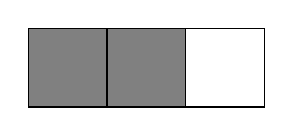
\begin{tikzpicture}
					\draw [draw=black] (3,1) rectangle (0,0);
					\draw [draw=black,fill=gray] (2,1) rectangle (0,0);
					\draw [] (1,1) -- (1,0);
					\draw [] (2,1) -- (2,0);
			\end{tikzpicture}}
		\caption[]{\textsc{\citeauthor{Lewis1988}-Relevant}\newline \textsc{\citeauthor{Roberts2012}-Relevant}\newline\textsc{Q-Relevant}.}\label{fig6:relevant-p}
	\end{subfigure}
	\hfill
	\begin{subfigure}[t]{.24\linewidth}
		\centering\scalebox{1}{
			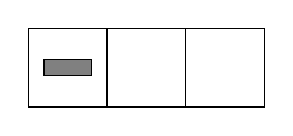
\begin{tikzpicture}
					\draw [draw=black] (3,1) rectangle (0,0);
					\draw [draw=black,fill=gray] (.8,.6) rectangle (.2,.4);
					\draw [] (1,1) -- (1,0);
					\draw [] (2,1) -- (2,0);
			\end{tikzpicture}}
		\caption[]{\textsc{\citeauthor{Lewis1988}-Irrelevant}\newline \textsc{\citeauthor{Roberts2012}-Relevant}\newline\textsc{Q-Irrelevant}.}
	\end{subfigure}\hfill
	\begin{subfigure}[t]{.24\linewidth}
		\centering\scalebox{1}{
			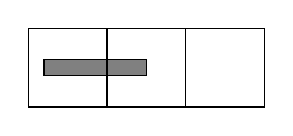
\begin{tikzpicture}
					\draw [draw=black] (3,1) rectangle (0,0);
					\draw [draw=black,fill=gray] (1.5,.6) rectangle (.2,.4);
					\draw [] (1,1) -- (1,0);
					\draw [] (2,1) -- (2,0);
			\end{tikzpicture}}
		\caption[]{\textsc{\citeauthor{Lewis1988}-Irrelevant}\newline \textsc{\citeauthor{Roberts2012}-Relevant}\newline\textsc{Q-Irrelevant}.}
	\end{subfigure}\hfill
	\begin{subfigure}[t]{.24\linewidth}
			\centering\scalebox{1}{
				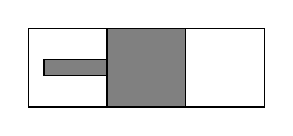
\begin{tikzpicture}
						\draw [draw=black] (3,1) rectangle (0,0);
						\draw [draw=black,fill=gray] (2,1) rectangle (1,0);
						\draw [draw=black,fill=gray] (1,.6) rectangle (.2,.4);
						\draw [] (1,1) -- (1,0);
						\draw [] (2,1) -- (2,0);
				\end{tikzpicture}}
			\caption[]{\textsc{\citeauthor{Lewis1988}-Irrelevant}\newline \textsc{\citeauthor{Roberts2012}-Relevant}\newline\textsc{Q-Relevant}.}
		\end{subfigure}
	\caption[]{Various QuD-proposition configurations (proposition/restrictor node defined by the gray area).}\label{fig6:qud-p-diagrams}
\end{figure}


We will see that this ``hybrid'' definition will be crucial to capture what we will call ``Compatible'' HCs (see Section \ref{sec6:chc}). Before showing how (\ref{ex6:incremental-q-relevance}) captures HCs, let us establish three useful results that will significantly simplify the argument. The first result, has to do with what we previously called \textsc{Vacuous tree-node intersection}, repeated below.

\begin{exe}
	\exr{ex2:vacuous-tree-node} {\textsc{\textbf{Vacuous tree-node intersection}}. Let $T$ be a Qtree whose leaves are $\mathcal{L}(T)$, and $N$ a (non-empty) node (set of worlds). $T\cap N = N$ iff $\exists N' \in \mathcal{L}(T). \ N \vDash N'$.}
\end{exe}

Let us consider a specific subcase of the condition stated in (\ref{ex2:vacuous-tree-node}), namely, the case in which the restrictor node at stake \textit{strictly} entails some leaf in the Qtree it gets intersected with. In that case, tree-node intersection is vacuous, but also, \textsc{Irrelevant}. This is because it results in a single node, that is a strict subset of the leaf it entails. In other words, the final result does not preserve any leaf from the input Qtree. This is repeated in (\ref{ex6:irrelevant-inter-simple}), and will prove very handy when dealing with HCs.

\begin{exe}
	\ex\label{ex6:irrelevant-inter-simple} {\textit{Irrelevance by} \textsc{\textbf{Single Strict Entailment}}. Let $T$ be a Qtree whose leaves are $\mathcal{L}(T)$, and $N$ a (non-empty) node (set of worlds). If $\exists N' \in \mathcal{L}(T). \ N \vDash N' \wedge N \not\equiv N'$, then $T\cap N$ is \textsc{Irrelevant}.}
\end{exe}

This subcase has an interesting generalization, that will prove useful when analyzing ``Compatible'' HCs in Section \ref{sec6:chc}. Suppose now the restrictor node at stake can be partitioned into a set of propositions, s.t. each of them strictly entails a leaf in the Qtree the node gets intersected with. In that case, tree-node intersection will \textit{not} be vacuous, because the node does not entail a single leaf. It will be \textsc{Irrelevant} however. This is because, if the node $N$ in question, can be partitioned into a set $\lbrace N_1, N_2, ..., N_k\rbrace$ of propositions, each of which strictly entails the leaves $\lbrace L_1, L_2, ..., L_k\rbrace$ in $T$, respectively, then, the intersection between $N$ and $T$, will simply be the Qtree whose leaves are $\lbrace N_1, N_2, ..., N_k\rbrace$. Since none of these nodes fully coincides with a leaf in $T$, due to the assumption of strict entailment, the tree-node intersection operation fails to be \textsc{Relevant}. This is summarized in (\ref{ex6:irrelevant-inter-complex}).

\begin{exe}
	\ex\label{ex6:irrelevant-inter-complex} {\textit{Irrelevance by} \textsc{\textbf{Multiple Strict Entailment}}. Let $T$ be a Qtree whose leaves are $\mathcal{L}(T)$, and $N$ a (non-empty) node (set of worlds). If $\exists \lbrace N_1, N_2, ..., N_k \rbrace$ a partition of $N$ and $\exists \lbrace L_1, L_2, ..., L_k \rbrace \subset \mathcal{L}(T)$ s.t. $\forall i \in [1; k]. \ N_i \vDash L_i \wedge N_i \not\equiv L_i$, then $T\cap N$ is \textsc{Irrelevant}.}
\end{exe}

Lastly, let us consider one more case that will turn out useful when analyzing HCs. We now assume that the restrictor node at stake in tree-node intersection, is compatible with all the leaves in the Qtree is gets intersected with. In that case, tree-node intersection may shrink some leaves of the input Qtree, but, all leaves in the original Qtree, will still intersect with some leaf in the output Qtree, due to the assumption of compatibility. In other words, the intersection operation will not exclude any leaf. It will thus be deemed \textsc{Irrelevant}. This is summarized in (\ref{ex6:irrelevant-compat}). 

\begin{exe}
	\ex\label{ex6:irrelevant-compat} {\textit{Irrelevance by} \textsc{\textbf{Holistic Compatibility}}. Let $T$ be a Qtree whose leaves are $\mathcal{L}(T)$, and $N$ a (non-empty) node (set of worlds). If $\forall L \in \mathcal{L}(T). \ L \wedge N \not\vDash \bot$, then $T\cap N$ is \textsc{Irrelevant}.}
\end{exe}

We are now equipped with the tools and definitions to smoothly deal with HCs. 

\subsection{Capturing the contrast in Hurford Conditionals}

We now explain the oddness pattern of the HCs in (\ref{ex6:hc}). We start with the felicitous HC (\ref{ex6:hc-ws}), whose Qtrees are repeated in Figure \ref{fig6:qtrees-hc-ws-r} below. In such Qtrees, the depth-$2$ layer, was obtained by intersecting a Qtree for the consequent (\textit{not Noto}), with the \textit{Italy}-node verifying the antecedent. 

\begin{figure}[H]
	\centering
	\begin{subfigure}[b]{.45\linewidth}
		\centering
		\scalebox{1}
		{\begin{forest}
				[CS [\textcolor{blue}{Italy} [\textcolor{orange}{Noto}][\fbox{$\neg$\textcolor{orange}{Noto}$\cap$\textcolor{blue}{Italy}}]] [{$\neg$\textcolor{blue}{Italy}} ]]
		\end{forest}}
		\caption[]{Tree \ref{fig6:qtree-italy-polar} $\rightarrow$ Tree \ref{fig6:qtree-not-noto-polar}.\\\textsc{\textbf{Q-Irrelevant}}.}\label{fig6:tree-hc-ws-polar-polar-r}
	\end{subfigure}\hfill
	\begin{subfigure}[b]{.45\linewidth}
		\centering
		\scalebox{1}
		{\begin{forest}
				[CS [\textcolor{blue}{Italy} [\textcolor{orange}{Noto}] [\fbox{\textcolor{orange}{Rome}}] [\fbox{\textcolor{orange}{...}}]] [{$\neg$\textcolor{blue}{Italy}} ]]
		\end{forest}}
		\caption[]{Tree \ref{fig6:qtree-italy-polar} $\rightarrow$ Tree \ref{fig6:qtree-not-noto-wh}/\ref{fig6:qtree-not-noto-tiered}.\\\textsc{\textbf{Q-Relevant}}.}\label{fig6:tree-hc-ws-polar-wh-r}
	\end{subfigure}
\end{figure}
\begin{figure}[H]
\ContinuedFloat
\centering	
	\begin{subfigure}[b]{.45\linewidth}
		\centering
		\scalebox{1}
		{\begin{forest}
				[CS [\textcolor{blue}{Italy}[\textcolor{orange}{Noto}][\fbox{$\neg$\textcolor{orange}{Noto}$\cap$\textcolor{blue}{Italy}}]] [\textcolor{blue}{France}] [\textcolor{blue}{...}]]
		\end{forest}}
		\caption[]{Tree \ref{fig6:qtree-italy-wh} $\rightarrow$ Tree \ref{fig6:qtree-not-noto-polar}.\\\textsc{\textbf{Q-Irrelevant}}.}\label{fig6:tree-hc-ws-wh-polar-r}
	\end{subfigure}\hfill
	\begin{subfigure}[b]{.45\linewidth}
		\centering
		\scalebox{1}
		{\begin{forest}
				[CS [\textcolor{blue}{Italy}[\textcolor{orange}{Noto}] [\fbox{\textcolor{orange}{Rome}}] [\fbox{\textcolor{orange}{...}}]] [\textcolor{blue}{France}] [\textcolor{blue}{...}] ]
		\end{forest}}
		\caption[]{Tree \ref{fig6:qtree-italy-wh} $\rightarrow$ Tree \ref{fig6:qtree-not-noto-wh}/\ref{fig6:qtree-not-noto-tiered}.\\\textsc{\textbf{Q-Relevant}}.}\label{fig6:tree-hc-ws-wh-wh-r}
	\end{subfigure}
	\caption[]{Qtrees for (\ref{ex6:hc-ws})=\textit{If SuB29 will take place in Italy, it will not take place in Noto}.}
	\label{fig6:qtrees-hc-ws-r}
\end{figure}

Let us now review each Qtree and see whether the tree-node intersection operation used to form it, is \textsc{Relevant}. Note that it is enough to find one well-formed Qtree for (\ref{ex6:hc-ws}) to be correctly predicted to be felicitous.

Starting with the Qtree in Figure \ref{fig6:tree-hc-ws-polar-polar-r}, this Qtree was obtained by intersecting the ``polar'' Qtree for \textit{not Noto}, with \textit{Italy}. Because \textit{Italy} is compatible with both \textit{Noto} and \textit{not Noto}, the \textsc{Holistic Compatibility} property (\ref{ex6:irrelevant-compat}) predicts the intersection operation to be \textsc{Irrelevant}. So this Qtree is odd given (\ref{ex6:hc-ws}).

Now considering the Qtree in Figure \ref{fig6:tree-hc-ws-polar-wh-r}; this Qtree was obtained by intersecting the ``\textit{wh}'' (articulated or not) Qtree for \textit{not Noto}, with \textit{Italy}. The resulting set of leaves, is the partition of \textit{Italy} made of Italian cities. This set of leaves, makes the intersection operation \textsc{Relevant}: all Italian cities were leaves in the original ``\textit{wh}'' (articulated or not) Qtree for \textit{not Noto}, and additionally, the original ``\textit{wh}'' Qtree for \textit{not Noto}, contained non-Italian city leaves, that were properly excluded by the intersection operation. Therefore, the Qtree in Figure \ref{fig6:tree-hc-ws-polar-wh-r}, does not violate \textsc{Incremental Q-Relevance}, and (\ref{ex6:hc-ws}) is correctly predicted not to be felicitous.

We could stop here, but let us review the Qtrees in Figures \ref{fig6:tree-hc-ws-wh-polar-r} and \ref{fig6:tree-hc-ws-wh-wh-r} for completeness. Turning to the Qtree in Figure \ref{fig6:tree-hc-ws-wh-polar-r}; it was obtained by intersecting the ``polar'' Qtree for \textit{not Noto}, with \textit{Italy} -- just like the Qtree in Figure \ref{fig6:tree-hc-ws-polar-polar-r}. The intersection operation is therefore predicted to be \textsc{Irrelevant} too.

Lastly, the Qtrees in Figure \ref{fig6:tree-hc-ws-wh-wh-r} was obtained by intersecting the ``\textit{wh}'' (articulated or not) Qtree for \textit{not Noto}, with \textit{Italy} -- just like the Qtree in Figure \ref{fig6:tree-hc-ws-polar-wh-r}. The intersection operation is therefore predicted to be \textsc{Relevant}, too.\\

We now proceed to analyzing the infelicitous HC (\ref{ex6:hc-sw}), whose Qtrees are repeated in Figure \ref{fig6:qtrees-hc-sw-r} below. In the Qtrees in Figure \ref{fig6:tree-hc-sw-polar-polar-r} and \ref{fig6:tree-hc-sw-polar-wh-r}, the depth-$2$ layer, was obtained by intersecting a Qtree for the consequent (\textit{Italy}), with the \textit{not Noto}-node verifying the antecedent. In the Qtrees in Figures \ref{fig6:tree-hc-sw-wh-r} and \ref{fig6:tree-hc-sw-wh-wh-r}, all layers are contributed by the antecedent Qtree, because the intersection operation between city-level leaves and the country-level Qtree contributed by the consequent, was shown to be vacuous.

\begin{figure}[H]
	\centering
	\begin{subfigure}[b]{.45\linewidth}
		\centering
		\scalebox{1}
		{\begin{forest}
				[CS [\textcolor{orange}{Noto}] [{$\neg$\textcolor{orange}{Noto}} [\fbox{\textcolor{blue}{Italy}$\cap\neg$\textcolor{orange}{Noto}}][$\neg$\textcolor{blue}{Italy}]]]
		\end{forest}}
		\caption[]{Tree \ref{fig6:qtree-not-noto-polar} $\rightarrow$ Tree \ref{fig6:qtree-italy-polar}.\\\textsc{\textbf{Q-Irrelevant}}.}\label{fig6:tree-hc-sw-polar-polar-r}
	\end{subfigure}\hfill
	\begin{subfigure}[b]{.45\linewidth}
		\centering
		\scalebox{1}
		{\begin{forest}
				[CS [\textcolor{orange}{Noto}] [{$\neg$\textcolor{orange}{Noto}} [\fbox{\textcolor{blue}{Italy}$\cap\neg$\textcolor{orange}{Noto}}][\textcolor{blue}{France}] [\textcolor{blue}{...}]]]
		\end{forest}}
		\caption[]{Tree \ref{fig6:qtree-not-noto-polar} $\rightarrow$ Tree \ref{fig6:qtree-italy-wh}.\\\textsc{\textbf{Q-Irrelevant}}.}\label{fig6:tree-hc-sw-polar-wh-r}
	\end{subfigure}
\end{figure}
\begin{figure}[H]
\ContinuedFloat
\centering	
	\begin{subfigure}[b]{.45\linewidth}
		\centering
		\scalebox{1}
		{\begin{forest}
				[CS [\textcolor{orange}{Noto}] [\fbox{\textcolor{orange}{Rome}}] [\fbox{\textcolor{orange}{...}}] [\textcolor{orange}{Paris}] [\textcolor{orange}{...}]]
		\end{forest}}
		\caption[]{Tree \ref{fig6:qtree-not-noto-wh} $\rightarrow$ Tree \ref{fig6:qtree-italy-polar}/\ref{fig6:qtree-italy-wh}.\\\textsc{\textbf{Q-Irrelevant}}.}\label{fig6:tree-hc-sw-wh-r}
	\end{subfigure}\hfill
	\begin{subfigure}[b]{.45\linewidth}
		\centering
		\scalebox{1}
		{\begin{forest}
				[CS [\textcolor{blue}{Italy}[\textcolor{orange}{Noto}] [\fbox{\textcolor{orange}{Rome}}] [\fbox{\textcolor{orange}{...}}]]  [\textcolor{blue}{France}[\textcolor{orange}{Paris}][\textcolor{orange}{...}]] [\textcolor{blue}{...}]]
		\end{forest}}
		\caption[]{Tree \ref{fig6:qtree-not-noto-tiered} $\rightarrow$ Tree \ref{fig6:qtree-italy-polar}/\ref{fig6:qtree-italy-wh}.\\\textsc{\textbf{Q-Irrelevant}}.}\label{fig6:tree-hc-sw-wh-wh-r}
	\end{subfigure}
	\caption[]{Qtrees for (\ref{ex6:hc-sw})=\#\textit{If SuB29 will not take place in Noto, it will take place in Italy}.}
	\label{fig6:qtrees-hc-sw-r}
\end{figure}


Let us now review each Qtree and show that, in each case, the tree-node intersection operation used to form it, was \textsc{Irrelevant}.

Starting with the Qtree in Figure \ref{fig6:tree-hc-sw-polar-polar-r}, this Qtree was obtained by intersecting the ``polar'' Qtree for \textit{Italy}, with \textit{not Noto}. Because \textit{not Noto} is compatible with both \textit{Italy} and \textit{not Italy}, the \textsc{Holistic Compatibility} property (\ref{ex6:irrelevant-compat}) predicts the intersection operation to be \textsc{Irrelevant}. So this Qtree is ill-formed.

Now considering the Qtree in Figure \ref{fig6:tree-hc-sw-polar-wh-r}; this Qtree was obtained by intersecting the ``\textit{wh}'' Qtree for \textit{Italy}, with \textit{not Noto}. Again, because \textit{not Noto} is compatible with any country-level node, the \textsc{Holistic Compatibility} property (\ref{ex6:irrelevant-compat}) predicts the intersection operation to be \textsc{Irrelevant}. So this Qtree is ill-formed as well.\\

Turning to the Qtree in Figure \ref{fig6:tree-hc-sw-wh-r}; this Qtree was obtained by intersecting any Qtree for \textit{Italy} (polar or ``\textit{wh}''), with city-leaves that are not \textit{not Noto}. Let us start by considering the intersection between a city-leaf, and a polar Qtree for \textit{Italy}, whose leaves are \textit{Italy} and \textit{not Italy}. Because any city, strictly entails \textit{Italy} or strictly entails \textit{not Italy}, the \textsc{Single Strict Entailment} property (\ref{ex6:irrelevant-inter-simple}) predicts the intersection operation to be \textsc{Irrelevant}. Now consider the intersection between a city-leaf, and a ``\textit{wh}'' Qtree for \textit{Italy}, whose leaves are country-level. Because any city, strictly entails some country, the \textsc{Single Strict Entailment} property (\ref{ex6:irrelevant-inter-simple}), again predicts the intersection operation to be \textsc{Irrelevant}. So, no matter how it gets derived, the Qtree in Figure \ref{fig6:tree-hc-sw-wh-r}, is derived \textit{via} an \textsc{Irrelevant} tree-node intersection operation. So this Qtree is ill-formed.

Lastly, the Qtree in Figure \ref{fig6:tree-hc-sw-wh-wh-r} was obtained by intersecting any Qtree for \textit{Italy} (polar or ``\textit{wh}''), with city-leaves that are not \textit{not Noto}. The intersections operations are thus exactly similar to those performed in Figure \ref{fig6:tree-hc-sw-wh-r}, and which were just shown to be \textsc{Irrelevant} as per the \textsc{Single Strict Entailment} property (\ref{ex6:irrelevant-inter-simple}). So, no matter how it gets derived, the Qtree in Figure \ref{fig6:tree-hc-sw-wh-wh-r}, is derived \textit{via} an \textsc{Irrelevant} tree-node intersection operation. So this Qtree is ill-formed.

Therefore all Qtrees derived for the infelicitous HC (\ref{ex6:hc-sw}), were derived \textit{via} an \textsc{Irrelevant} tree-node intersection operation. As a result, (\ref{ex6:hc-sw}) is not compatible with any well-formed Qtree, and as such should be deemed odd. The contrast observed in HCs is captured.

\subsection{Taking stock}

In this Section, we have shown that HCs could not be accounted for by previously posited constraints (\textsc{Empty Labeling}; \textsc{Q-Non-Redundancy}). We have then discussed how earlier notions or \textsc{Relevance} could help, \textit{modulo} stipulative assumptions. We then proposed a new notion of \textsc{Relevance}, \textsc{Incremental Q-Relevance}, that we framed as a constraint on the tree-node intersection operation, an operation recruited during the formation of conditional Qtrees. This way, we got the specific directionality of \textsc{Relevance}, for free. We then showed how this new view could capture the contrast in HCs. Specifically, we showed that some Qtrees evoked by the felicitous HC (\ref{ex6:hc-ws}), were derived \textit{via} an intersection operation that was properly ``shrinking'' the consequent Qtree -- retaining at least one leaf; excluding at least one leaf. And we showed that no Qtree evoked by the infelicitous HC (\ref{ex6:hc-sw}), could be derived in a similar fashion.\\

Zooming out, the asymmetry we derived in HC can be traced back to how Qtrees for \textit{Italy} ($p$) and \textit{(not) Noto} ($(\neg) p^+$) were defined: crucially, we observed beck in Section \ref{sec6:qtrees-hc}, that at least one Qtree for \textit{not Noto} formed a strict refinement of a Qtree for \textit{Italy} -- eventually leading to a \textsc{Relevant} tree-node intersection operation. This intuition is generalized in (\ref{ex6:refinement-relevance}), which roughly says that two Qtrees can be ``conditionalized'' if all the verifying nodes of the antecedent Qtree, are further subdivided in the consequent Qtree. 

\begin{exe}
	\ex {\textsc{Qtree Refinements and Incremental Q-Relevance}. Let $T$ be a Qtree whose verifying leaves are $\mathcal{N}^+(T)$, and all have depth at least $1$ (i.e. the root is not verifying). Let $T'$ be a Qtree whose root is the same as $T$, whose nodes include $\mathcal{N}^+(T)$, and are s.t. $\mathcal{L}(T')\cap\mathcal{N}^+(T)=\emptyset$, i.e. any node in $T'$ that is verifying in $T$, is further subdivided in $T'$. Then, a conditional Qtree can be formed out of $T$ (as antecedent) and $T'$ (as consequent).}\label{ex6:refinement-relevance}
	\ex {\textit{Proof of (\ref{ex6:refinement-relevance}).} Let $T$ be a Qtree whose verifying nodes are $\mathcal{N}^+(T)$, and all have depth at least $1$. Let $T'$ be a Qtree whose root is the same as $T$, whose nodes include $\mathcal{N}^+(T)$, and are s.t. $\mathcal{L}(T')\cap\mathcal{N}^+(T)=\emptyset$. To show that a conditional Qtree can be formed out of $T$ (as antecedent) and $T'$ (as consequent), we must show that the intersection between each verifying leaf of $T$ and $T'$, is \textsc{Relevant}. Because all verifying nodes in $T$ have the same characteristics in $T'$, it is enough to show that the intersection between an arbitrary verifying node in $T$, and $T'$, is \textsc{Relevant}. Let $N$ be such a node. By assumption, $N$ is in $T'$ and further subdivided in $T'$. So $T' \cap N$ is exactly the subtree of $T'$ rooted in $N$. Let us call this subtree $T''$. $T''$ contains at least a leaf from $T'$ (in fact, all its leaves, are leaves from $T'$). Additionally, $T''$ does not contain all leaves from $T'$. This is because all leaves from $T'$ partition the root of $T'$. Because $N$ is by assumption different from the root (i.e. a subset of the root), $T'' = T \cap N$'s leaves, partition a subset of the root. So $T'' = T \cap N$'s leaves, form a subset of $T'$'s leaves. Therefore, $T \cap N$ is \textsc{Relevant}, and the conditional Qtree formed out of $T$ (as antecedent) and $T'$ (as consequent), is well-formed.}
\end{exe}

A special case of this condition, is when the verifying nodes of the antecedent and consequent Qtree are all leaves, and when the consequent strictly refines the antecedent. In that case, the resulting conditional Qtree is defined. This is exactly the kind of configuration that felicitous HCs like (\ref{ex6:hc-ws}) give rise to: we observed that some Qtree for \textit{not Noto} formed a strict refinement of some Qtree for \textit{Italy}, and additionally, both Qtrees only had verifying leaves.

By contrast, when the verifying nodes of the antecedent and consequent Qtree are all leaves, and when the antecedent strictly refines the consequent, the resulting conditional Qtree is \textit{not} defined. This is exactly the kind of configuration that infelicitous HCs like (\ref{ex6:hc-sw}) give rise to: we observed that no Qtree for \textit{Italy} formed a (strict) refinement of a Qtree for \textit{not Noto} -- leading to \textsc{Irrelevant} tree-node intersection operations across the board. These general properties are spelled out in (\ref{ex6:refinement-relevance-opp}) and proved in (\ref{ex6:refinement-relevance-opp-proof}).


\begin{exe}
	\ex {\textsc{Strict Qtree Refinements and Incremental Q-Relevance}. Let $T$ and $T'$ be Qtrees that are more than just one root, whose verifying nodes are leaves and s.t. $T'$ strictly refines $T$. Then:
		\begin{enumerate}[(i)]
			\item no conditional Qtree can be formed out of $T'$ (as antecedent) and $T$ (as consequent);\label{ex6:refinement-relevance-neg}
			\item while a conditional Qtree can be formed out of $T$ (as antecedent) and $T'$ (as consequent). This is a special case of (\ref{ex6:refinement-relevance}).\label{ex6:refinement-relevance-pos}
		\end{enumerate}}\label{ex6:refinement-relevance-opp}
	\ex {\textit{Proof of (\ref{ex6:refinement-relevance-opp}).} Let $T$ and $T'$ be Qtrees that are more than just one root, whose verifying nodes are leaves and s.t. $T'$ strictly refines $T$.}
	\begin{xlist}
		 \ex {\textit{Proof of (\ref{ex6:refinement-relevance-opp}\ref{ex6:refinement-relevance-neg})}. Let $L'$ be verifying in $T'$. Because $T'$ strictly refines $T$, $L'$ cannot be a leaf in $T$, and must strictly entail a leaf in $T$. Therefore, $T \cap L'$ is \textsc{Irrelevant} as per the \textsc{Single Strict Entailment} property (\ref{ex6:irrelevant-inter-simple}). Therefore, the conditional Qtree $T' \rightarrow T$ is not defined.}
		 \ex {\textit{Proof of (\ref{ex6:refinement-relevance-opp}\ref{ex6:refinement-relevance-pos})}. Let $L$ be verifying in $T$. Because $T'$ strictly refines $T$, $L$ also belongs to $T'$, and has at least two children in $T'$. Therefore, $T' \cap L$ is the subtree of $T'$ rooted in $L$, that is more than just one root. The leaves of this subtree are all leaves of $T'$, and additionally, are not \textit{all} leaves of $T'$, otherwise $L$ would have been $T$/$T'$'s root, contrary to assumptions. Therefore, $T' \cap L$ is \textsc{Relevant} and the conditional Qtree $T \rightarrow T'$ is defined.}
	\end{xlist}\label{ex6:refinement-relevance-opp-proof}
\end{exe}

In summary, if the verifying, ``restrictor'' nodes provided by the antecedent Qtree, are too fine-grained for the consequent Qtree, the tree-node intersection operations performed when building a conditional Qtree, will be \textsc{Irrelevant}, and the entire derivation will crash. This leads us to mention a couple more important observations about how \textsc{Incremental Q-Relevance} operates. First, even if \textsc{Incremental Q-Relevance} restricts tree-node intersection, where the tree is contributed by the consequent and the restrictor node (a proposition) is contributed by the antecedent, it is indirectly sensitive to the structure of the antecedent Qtree, essentially because the verifying ``restrictor'' nodes passed to tree-node intersection, are determined by how fine-grained the antecedent's Qtree is. If the antecedent is fined-grained like \textit{(not) Noto}, the verifying nodes of its Qtrees will be fine-grained as well, meaning, the restrictor nodes passed to tree-node intersection, will be fine-grained. This in turn will make tree-node intersection less likely to achieve \textsc{Relevance}. In that sense, \textsc{Incremental Q-Relevance} is conceptually different from \citeauthor{Lewis1988}'s and \citet{Roberts2012}'s approaches to ``assertive'' \textsc{Relevance},\footnote{Both \citeauthor{Lewis1988} and \citet{Roberts2012} however proposed \textsc{Relevance} constraints between question-types. For Roberts for instance, a follow-up question is \textsc{Relevant} to a QuD, if all the alternatives in the denotation of that follow-up question, are \textsc{\citeauthor{Roberts2012}-Relevant} (as defined in (\ref{ex1:roberts-relevance})). This brings us a bit closer to what was done here. \citeauthor{Lewis1988}'s approach is further described and analyzed in Appendix \ref{sec6:lewis}.} which treated a \textsc{Relevant} or \textsc{Irrelevant} proposition simply as a set of worlds, and not as a set of nodes (i.e. a set of sets of worlds).

A second, yet observation, is that \textsc{Incremental Q-Relevance} being a constraint on tree-node intersection, it will have to be checked for every single tree-node intersection operation performed as part of the formation of a conditional Qtree. If one of these operations fails to be \textsc{Relevant}, then the derivation of the entire conditional Qtree, will be expected to fail. There will be as many such operations, as there are verifying, ``restrictor'' nodes in the antecedent Qtree. In particular, increasing the complexity of the antecedent, may increase the number of verifying nodes. In that respect, an interesting subcase is that of a disjunctive antecedent mixing different levels of granularity. In such cases, the finer-grained component will determine what the finest-grained restrictor nodes are, and as such, will constitute the bottleneck for \textsc{Incremental Q-Relevance}. We will see a few examples instantiating that observation in the next Section.


\section{Extension to ``Compatible'' Hurford Conditionals}\label{sec6:chc}

In this Section, we explore the predictions of \textsc{Incremental Q-Relevance} on data that might look familiar from Chapter \ref{chap:hurford-disj}, that the other prominent account of HCs, \textsc{Super-Redundancy}, is shown to struggle with.

\subsection{``Compatible'' Hurford Disjunctions and their disjunctwise negated counterparts}

In Chapter \ref{chap:hurford-disj}, we introduced ``Compatible'' Hurford Disjunctions (henceforth \textbf{CHD}s), repeated below. Such disjunctions feature merely compatible disjuncts, and still feel odd. Chapter \ref{chap:hurford-disj} predicted the sentences in (\ref{ex5:chd}) to be odd, due to them featuring disjuncts conveying incomparable degrees of granularity, which in turn made it impossible to derive well-formed disjunctive Qtrees for these sentences. Most if not all accounts of pragmatic oddness, including \textsc{Super-Redundancy}, struggle with such sentences.

\begin{exe}
	\exr{ex5:chd}
	\begin{xlist}
		\ex[\#] {SuB29 will take place in the Basque country or France. \hfill $\q\vee\p$; $\q \wedge \p \not\vDash\bot$}
		\ex[\#] {SuB29 will take place in France or in the Basque country. \hfill $\p\vee\q$; $\p \wedge \q \not\vDash\bot$}
	\end{xlist}
\end{exe} 

Just like regular HDs, CHDs have ``disjunctwise'' negated counterparts, given in (\ref{ex6:chd-neg}). We will call such expressions \textbf{DNCHD}s. The DNCHDs in (\ref{ex6:chd-neg}) still meet the description of CHDs, because, if $p$ and $q$ are merely compatible, so do $\neg p$ and $\neg q$.

\begin{exe}
	\ex\label{ex6:chd-neg}
	\begin{xlist}
		\ex[\#] {SuB29 won't take place in the Basque country or won't take place in France. \hfill $(\neg\q)\vee(\neg\p)$; $(\neg\q) \wedge (\neg\p) \not\vDash\bot$}
		\ex[??] {SuB29 won't take place in France or won't take place in the Basque country. \hfill $(\neg\p)\vee(\neg\q)$; $(\neg\p) \wedge (\neg\q) \not\vDash\bot$}
	\end{xlist}
\end{exe} 

Our account predicts the sentences in (\ref{ex6:chd-neg}) to be just as bad as those in (\ref{ex5:chd}), for the same reasons: their two disjuncts convey incomparable degrees of granularity -- inherited from their unnegated counterparts. Therefore, none of the variants in (\ref{ex6:chd-neg}) can evoke a well-formed disjunctive Qtree. \citeauthor{Kalomoiros2024}'s \textsc{Super-Redundancy} on the other hand, predicts both sentences to be fine. This is detailed in (\ref{ex6:chd-neg-sr}).

\begin{exe}
	\ex\label{ex6:chd-neg-sr} {DNCHDs are not Super Redundant (SR).\\
		We show (\ref{ex6:chd-neg})=$(\neg\p)\vee(\neg\q)$, with $(\neg\p) \wedge (\neg\q) \not\vDash \bot$, is not SR.\\
		Take C = $\neg\p$.\\
		We then have (\ref{ex6:hd-neg})$^-_C$ = $\neg\q$.\\
		Take $D=\bot$.\\
		$(\textref{ex6:chd-neg})_{Str(C, D)} = (\neg(\p \wedge D)) \vee (\neg\q)$\\
		\phantom{$(\textref{ex6:chd-neg})_{Str(C, D)}$} $\equiv (\neg(\p \wedge \bot)) \vee (\neg\q)$\\
		\phantom{$(\textref{ex6:chd-neg})_{Str(C, D)}$} $\equiv (\neg\bot) \vee (\neg\q)$\\
		\phantom{$(\textref{ex6:hd-neg})_{Str(C, D)}$} $\equiv \top \vee (\neg\q)$\\
		\phantom{$(\textref{ex6:hd-neg})_{Str(C, D)}$} $\equiv \top$\\
		\phantom{$(\textref{ex6:hd-neg})_{Str(C, D)}$} $\not\equiv \neg\q = (\textref{ex6:chd-neg})^-_C$\\
		Exact same reasoning when taking C = $\neg\q$, swapping the roles of \p{} and \q.
	}
\end{exe}

What about conditional variants of the sentences in (\ref{ex5:chd}) and (\ref{ex6:chd-neg}), obtained \textit{via} the \textit{or}-to-\textit{if} tautology?

\subsection{Constructing ``Compatible'' HCs from CHDs}

Because we assumed that the formation of conditional Qtrees is distinct from that of disjunctive Qtrees, changing the disjunctions in (\ref{ex5:chd}) and (\ref{ex6:chd-neg}) into conditionals, may lead to different predictions. We now apply the \textit{or}-to-\textit{if} tautology to the sentences in (\ref{ex5:chd}) and (\ref{ex6:chd-neg}), to create four different kinds of ``Compatible'' Hurford Conditionals (henceforth \textbf{CHC}s). Note that we can generate four variants instead of just two (as it was the case for simple HCs derived out of HDs and DNHDs), because the two disjuncts in CHDs and DNCHDs, are not in any kind of entailment relation, and therefore play interchangeable roles. In other words, either disjunct can appear as an antecedent or consequent in the derived conditionals. Such conditionals are given in (\ref{ex6:chc}).

\begin{exe}
	\ex\label{ex6:chc}
	\begin{xlist}
		\ex{Derived from (\ref{ex5:chd}), using \q{} as antecedent.\\
			\# If SuB29 will not take place in the Basque country, it will take place in France. \hfill $\neg\q\rightarrow\p$}\label{ex6:chc-nbtf}
		\ex{Derived from (\ref{ex5:chd}), using \p{} as antecedent.\\
			?If SuB29 will not take place in France, it will take place in the Basque country. \\
			\hfill $\neg\p\rightarrow\q$}\label{ex6:chc-nftb}
		\ex{Derived from (\ref{ex6:chd-neg}) and double negation elimination, using $\neg$\q{} as antecedent.\\
			\# If SuB29 will take place in the Basque country, it will not take place in France. \hfill $\q\rightarrow\neg\p$}\label{ex6:chc-btnf}
		\ex{Derived from (\ref{ex6:chd-neg}) and double negation elimination, using $\neg$\p{} as antecedent.\\
			If SuB29 will take place in France, it will not take place in the Basque country. \hfill $\p\rightarrow\neg\q$}\label{ex6:chc-ftnb}
	\end{xlist}
\end{exe} 


Interestingly, the four CHCs in (\ref{ex6:chc}), seem to contrast in terms of felicity. Although the judgments may be subtle, it appears that the variants featuring \textit{France} in their antecedent ((\ref{ex6:chc-nftb}) and (\ref{ex6:chc-ftnb})), are less degraded than the variants featuring \textit{the Basque country} in their antecedent ((\ref{ex6:chc-nbtf}) and (\ref{ex6:chc-btnf})). The felicitous variants (\ref{ex6:chc-nftb}) and (\ref{ex6:chc-ftnb}), seem to be understandable as (\ref{ex6:chc-nftbnf}) and (\ref{ex6:chc-ftnbf}), respectively.


\begin{exe}
	\ex
	\begin{xlist}
		\ex{If SuB29 will not take place in France, it will take place in the Spanish Basque country. \hfill $\neg \p \rightarrow (\neg \p \wedge \q)$}\label{ex6:chc-nftbnf}
		\ex{If SuB29 will take place in France, it will not take place in the French Basque country. \hfill $\p \rightarrow \neg(\p \wedge \q)$}\label{ex6:chc-ftnbf}
	\end{xlist}
\end{exe}

Under the material implication hypothesis, \textsc{Super-Redundancy} predicts all variants in (\ref{ex6:chc}) to be fine, simply because the CHDs they are derived from, are already mispredicted by this account to be fine. This is shown for (\ref{ex6:chc-nbtf}) in (\ref{ex6:chc-nbtf-sr}) and for (\ref{ex6:chc-btnf}) in (\ref{ex6:chc-btnf-sr}). This trivially extends to the two other variants (\ref{ex6:chc-nftb}) and (\ref{ex6:chc-ftnb}) by simply swapping the roles of $p$ and $q$ in the proofs.\\

\begin{exe}
	\ex{CHCs are not Super Redundant (SR).}
		\begin{xlist}
			\ex {We show (\ref{ex6:chc-nbtf})=$(\neg\q)\rightarrow \p$, with $\p \wedge \q \not\vDash \bot$, is not SR.\\
				Take C = $\neg\q$.\\
				We then have (\ref{ex6:chc-nbtf})$^-_C$ = $\p$.\\
				Take $D=\top$.\\
				$(\textref{ex6:chc-nbtf})_{Str(C, D)} = (\neg(\q \wedge D)) \rightarrow \p$\\
				\phantom{$(\textref{ex6:chc-nbtf})_{Str(C, D)}$} $\equiv (\neg(\q \wedge \top)) \rightarrow \p$\\
				\phantom{$(\textref{ex6:chc-nbtf})_{Str(C, D)}$} $\equiv (\neg \q) \rightarrow \p$\\
				\phantom{$(\textref{ex6:chc-nbtf})_{Str(C, D)}$} $\not\equiv \p = (\textref{ex6:chc-nbtf})^-_C$\\
				Take C = $\p$.\\
				We then have (\ref{ex6:chc-nbtf})$^-_C$ = $\neg\q$.\\
				Take $D=\top$.\\
				$(\textref{ex6:chc-nbtf})_{Str(C, D)} = (\neg\q) \rightarrow (\p \wedge D)$\\
				\phantom{$(\textref{ex6:chc-nbtf})_{Str(C, D)}$} $\equiv (\neg\q) \rightarrow (\p \wedge \top)$\\
				\phantom{$(\textref{ex6:chc-nbtf})_{Str(C, D)}$} $\equiv (\neg\q) \rightarrow \p$\\
				\phantom{$(\textref{ex6:chc-nbtf})_{Str(C, D)}$} $\not\equiv \neg\q = (\textref{ex6:chc-nbtf})^-_C$}\label{ex6:chc-nbtf-sr} 
			\ex {We show (\ref{ex6:chc-btnf})=$\q\rightarrow (\neg\p)$, with $\p \wedge \q \not\vDash \bot$, is not SR.\\
				Take C = $\q$.\\
				We then have (\ref{ex6:chc-btnf})$^-_C$ = $\neg\p$.\\
				Take $D=\top$.\\
				$(\textref{ex6:chc-btnf})_{Str(C, D)} = (\q \wedge D) \rightarrow (\neg\p)$\\
				\phantom{$(\textref{ex6:chc-btnf})_{Str(C, D)}$} $\equiv (\q \wedge \top) \rightarrow (\neg\p)$\\
				\phantom{$(\textref{ex6:chc-btnf})_{Str(C, D)}$} $\equiv \q \rightarrow (\neg\p)$\\
				\phantom{$(\textref{ex6:chc-btnf})_{Str(C, D)}$} $\not\equiv \neg\p = (\textref{ex6:chc-btnf})^-_C$\\
				Take C = $\neg\p$.\\
				We then have (\ref{ex6:chc-nbtf})$^-_C$ = $\q$.\\
				Take $D=\top$.\\
				$(\textref{ex6:chc-btnf})_{Str(C, D)} = \q \rightarrow \neg(\p \wedge D)$\\
				\phantom{$(\textref{ex6:chc-btnf})_{Str(C, D)}$} $\equiv \q \rightarrow \neg(\p \wedge \top)$\\
				\phantom{$(\textref{ex6:chc-btnf})_{Str(C, D)}$} $\equiv \q \rightarrow \neg \p$\\
				\phantom{$(\textref{ex6:chc-btnf})_{Str(C, D)}$} $\not\equiv \q = (\textref{ex6:chc-btnf})^-_C$}\label{ex6:chc-btnf-sr}
		\end{xlist}
\end{exe}


From our perspective, this pattern may also look surprising, because we just established that \textsc{Relevance} in conditionals was associated with ``granularity'' violations (specifically, cases in which the antecedent was finer-grained than the consequent), and moreover, Chapter \ref{chap:hurford-disj} established that \textit{SuB29 will take place in France}, and \textit{SuB29 will take place in the Basque country}, conveyed \textit{orthogonal} degrees of granularity, that could not be reconciled. So, at first blush, we may have expected all the conditionals in (\ref{ex6:chc}) to pattern the same.

\subsection{Capturing CHCs}

We will now see that our model of evoked Qtrees, complemented with \textsc{Incremental Q-Relevance} \textit{actually} captures the pattern in (\ref{ex6:chc}). This will boil down to the fact that, although \textit{SuB29 will take place in France}, and \textit{SuB29 will take place in the Basque country} do not evoke Qtrees in any kind of refinement relation, \textit{SuB29 will take place in France} can be seen as ``coarser-grained'' than \textit{SuB29 will take place in the Basque country}, in the following, weaker sense: some regions like the Basque country, can be included in the union of two countries, but it is harder to think of a country that would be included in the union of two (or more) regions.\footnote{Note that this difference may be even more obvious when considering similar configurations, but at different levels of granularity, e.g. by adopting \citeauthor{Singh2008a}'s original examples involving countries like Russia, and continents like Asia. Some countries are included in the union of two continents, but no continent is included in the union of two (or more) countries. Here, we just kept France and the Basque country to stay in the theme.} We will see that this observation can be related to the property of \textsc{Multiple Strict Entailment} in (\ref{ex6:irrelevant-inter-complex}), that we showed caused \textsc{Irrelevance} in tree-node intersection. This will be enough to derive that the tree-node intersection operations performed when deriving Qtrees for (\ref{ex6:chc-nftb}) and (\ref{ex6:chc-ftnb}), are \textsc{Relevant}, while those performed in when deriving Qtrees for (\ref{ex6:chc-nbtf}) and (\ref{ex6:chc-btnf}), are not.\footnote{This prediction will follow from the concept of \textsc{Relevance} defined here, but does not follow from the previous version of this principle proposed in \citet{HenotMortier2024a}.}\\

To this end, let us first repeat the Qtrees for $S_p$ = \textit{SuB29 will take place in France} and $S_q$ = \textit{SuB29 will take place in the Basque country}, already derived in Chapter \ref{chap:hurford-disj}. Such Qtrees are given in Figure \ref{fig6:qtrees-france} and \ref{fig6:qtrees-basque}  respectively.



\begin{figure}[H]
	\centering
	\begin{subfigure}[b]{.45\linewidth}
		\centering
		\scalebox{1}{
			\begin{forest}
				[CS [\fbox{\textcolor{blue}{France}}] [$\neg$\textcolor{blue}{France}]]
			\end{forest}
		}\caption[]{``Polar''.}\label{fig6:qtree-france-polar}
	\end{subfigure}\hfill
	\begin{subfigure}[b]{.45\linewidth}
		\centering
		\scalebox{1}{
			\begin{forest}
				[CS [{\textcolor{blue}{Spain}}] [\fbox{\textcolor{blue}{France}}][\textcolor{blue}{...}]]
			\end{forest}
		}\caption[]{``\textit{Wh}''.}\label{fig6:qtree-france-wh}
	\end{subfigure}
	\caption[]{Qtrees evoked by $S_{\p}$ = \textit{SuB29 will take place in France}.}\label{fig6:qtrees-france}
\end{figure}

\begin{figure}[H]
	\centering
	\begin{subfigure}[b]{.25\linewidth}
		\centering
		\scalebox{1}{
			\begin{forest}
				[CS [\fbox{\textcolor{red}{Basque}}] [$\neg${\textcolor{red}{Basque}}]]
		\end{forest}}
		\caption[]{``Polar''.}\label{fig6:qtree-basque-polar}
	\end{subfigure}\hfill
	\begin{subfigure}[b]{.65\linewidth}
		\centering
		\scalebox{1}{
			\begin{forest}
				[CS [\fbox{\textcolor{red}{Basque country}}] [\textcolor{red}{Navarre}] [\textcolor{red}{Midi}] [...]]
		\end{forest}}
		\caption[]{``\textit{Wh}''.}\label{fig6:qtree-basque-wh}
	\end{subfigure}
	\caption[]{Qtrees for $S_{\q}$ = \textit{SuB29 will take place in the Basque country}.}\label{fig6:qtrees-basque}
\end{figure}
 
Qtrees the negations of $S_p$ and $S_q$, are given in Figures \ref{fig6:qtrees-not-france} and \ref{fig6:qtrees-not-basque} respectively. 



\begin{figure}[H]
	\centering
	\begin{subfigure}[b]{.45\linewidth}
		\centering
		\scalebox{1}{
			\begin{forest}
				[CS [{\textcolor{blue}{France}}] [\fbox{$\neg$\textcolor{blue}{France}}]]
			\end{forest}
		}\caption[]{``Polar''.}\label{fig6:qtree-not-france-polar}
	\end{subfigure}\hfill
	\begin{subfigure}[b]{.45\linewidth}
		\centering
		\scalebox{1}{
			\begin{forest}
				[CS [\fbox{\textcolor{blue}{Spain}}] [{\textcolor{blue}{France}}][\fbox{\textcolor{blue}{...}}]]
			\end{forest}
		}\caption[]{``\textit{Wh}''.}\label{fig6:qtree-not-france-wh}
	\end{subfigure}
	\caption[]{Qtrees evoked by $\neg S_{\p}$ = \textit{SuB29 won't take place in France}.}\label{fig6:qtrees-not-france}
\end{figure}

\begin{figure}[H]
	\centering
	\begin{subfigure}[b]{.25\linewidth}
		\centering
		\scalebox{1}{
			\begin{forest}
				[CS [{\textcolor{red}{Basque}}] [\fbox{$\neg${\textcolor{red}{Basque}}}]]
		\end{forest}}
		\caption[]{``Polar''.}\label{fig6:qtree-not-basque-polar}
	\end{subfigure}\hfill
	\begin{subfigure}[b]{.65\linewidth}
		\centering
		\scalebox{1}{
			\begin{forest}
				[CS [{\textcolor{red}{Basque country}}] [\fbox{\textcolor{red}{Navarre}}] [\fbox{\textcolor{red}{Midi}}] [\fbox{...}]]
		\end{forest}}
		\caption[]{``\textit{Wh}''.}\label{fig6:qtree-not-basque-wh}
	\end{subfigure}
	\caption[]{Qtrees for $\neg S_{\q}$ = \textit{SuB29 won't take place in the Basque country}.}\label{fig6:qtrees-not-basque}
\end{figure}

We can now evaluate which sentences in (\ref{ex6:chc}) have their conditional Qtrees violate \textsc{Incremental Q-Relevance}. We start with the infelicitous variant (\ref{ex6:chc-nbtf}). (\ref{ex6:chc-nbtf})'s Qtrees should be derived by composing antecedent Qtrees for \textit{not Basque} (in Figure \ref{fig6:qtrees-not-basque}) with consequent Qtrees for \textit{France} (in Figure \ref{fig6:qtrees-france}).

First, let us consider Figure \ref{fig6:qtree-not-basque-polar} as antecedent and Figure \ref{fig6:qtree-france-polar} as consequent. In that case, the \textit{not Basque} node acts as the only restrictor node, and gets intersected with the polar partition \textit{France} vs. \textit{not France}. Because the set of \textit{not Basque} worlds is compatible with both \textit{France} and \textit{not France}, the intersection operation is \textsc{Irrelevant}, as per the \textsc{Holistic Compatibility} property (\ref{ex6:irrelevant-compat}).

Second, let us consider Figure \ref{fig6:qtree-not-basque-polar} as antecedent and Figure \ref{fig6:qtree-france-wh} as consequent. In that case, the \textit{not Basque} node again acts as the only restrictor node, and gets intersected with a by-country partition. Because the set of \textit{not Basque} worlds is compatible with any single country (including \textit{France} and \textit{Spain}), the intersection operation is \textsc{Irrelevant}, again as per the \textsc{Holistic Compatibility} property (\ref{ex6:irrelevant-compat}).

Third, let us consider Figure \ref{fig6:qtree-not-basque-wh} as antecedent and Figure \ref{fig6:qtree-france-polar} as consequent. In that case, the region-level nodes different from the Basque country act as restrictor nodes, and each gets intersected with the polar partition \textit{France} vs. \textit{not France}. For the intersection operation to be \textsc{Relevant}, any region different from the Basque country, should strictly coincide with either \textit{France} or \textit{not France}. This would be the only way keep one cell, and exclude one other cell, from the consequent's partition and satisfy \textsc{Incremental Q-Relevance}. But obviously, this cannot hold of all regions -- in fact, this hold of none of them. Therefore, the intersection operation is \textsc{Irrelevant}.

Fourth and lastly, let us consider Figure \ref{fig6:qtree-not-basque-wh} as antecedent and Figure \ref{fig6:qtree-france-wh}. In that case, the region-level nodes different from the Basque country act as restrictor nodes, and each gets intersected with a by-country partition. For the intersection operation to be \textsc{Relevant}, any region different from the Basque country, should contain at least one country, and exclude at least one country. This would be the only way keep one cell, and exclude one other cell, from the consequent's partition and satisfy \textsc{Incremental Q-Relevance}. But obviously, this cannot hold of all regions: many regions are strictly contained in one single country. Therefore, the intersection operation is \textsc{Irrelevant}. We have just shown that there is no way to derive a conditional Qtree for (\ref{ex6:chc-nbtf}) \textit{via} well-formed (i.e. \textsc{Relevant}) tree-node intersection operations. Thus, (\ref{ex6:chc-nbtf}) is correctly predicted to be odd.\\

Now turning to the other infelicitous variant (\ref{ex6:chc-btnf}). (\ref{ex6:chc-btnf})'s Qtrees should be derived by composing antecedent Qtrees for \textit{Basque} (in Figure \ref{fig6:qtrees-basque}) with consequent Qtrees for \textit{not France} (in Figure \ref{fig6:qtrees-not-france}).

First, let us consider Figure \ref{fig6:qtree-basque-polar} as antecedent and Figure \ref{fig6:qtree-not-france-polar} as consequent. In that case, the \textit{Basque} node acts as the only restrictor node, and gets intersected with the polar partition \textit{France} vs. \textit{not France}. Because the set of \textit{Basque} worlds is compatible with both \textit{France} and \textit{not France}, the intersection operation is \textsc{Irrelevant}, as per the \textsc{Holistic Compatibility} property (\ref{ex6:irrelevant-compat}).

Second, let us consider Figure \ref{fig6:qtree-basque-polar} as antecedent and Figure \ref{fig6:qtree-not-france-wh} as consequent. In that case, the \textit{Basque} node again acts as the only restrictor node, and gets intersected with a by-country partition. Crucially here, because the set of \textit{Basque} worlds can be partitioned into two subsets, namely, \textit{the French Basque country} and \textit{the Spanish Basque country}, each of which strictly entails a leaf in the consequent's Qtree (namely, \textit{France} and \textit{Spain}), the intersection operation is \textsc{Irrelevant}, as per the \textsc{Multiple Strict Entailment} property (\ref{ex6:irrelevant-inter-complex}).

Third, let us consider Figure \ref{fig6:qtree-basque-wh} as antecedent and Figure \ref{fig6:qtree-not-france-polar} as consequent. In that case, the \textit{Basque} node again acts as the only restrictor node, and gets intersected with the polar partition \textit{France} vs. \textit{not France}. We have already established that this is \textsc{Irrelevant}.

Fourth and lastly, let us consider Figure \ref{fig6:qtree-basque-wh} as antecedent and Figure \ref{fig6:qtree-not-france-wh}. In that case, the \textit{Basque} node again acts as the only restrictor node, and gets intersected with a by-country partition. We have already established that this is \textsc{Irrelevant}. We have just shown that there is no way to derive a conditional Qtree for (\ref{ex6:chc-btnf}) \textit{via} well-formed (i.e. \textsc{Relevant}) tree-node intersection operations. Thus, (\ref{ex6:chc-btnf}) is correctly predicted to be odd.\\

Let us now show that the felicitous variants (\ref{ex6:chc-nftb}) and (\ref{ex6:chc-ftnb}) \textit{can} evoke conditional Qtrees derived \textit{via} \textsc{Relevant} tree-node intersection operations. In the case of (\ref{ex6:chc-nftb}), let us consider the polar Qtree for \textit{not France} in Figure \ref{fig6:qtree-not-france-polar} as antecedent Qtree, and the ``\textit{wh}'' Qtree for \textit{the Basque country} in Figure \ref{fig6:qtree-basque-wh}, as consequent Qtree. The resulting conditional Qtree is represented in Figure \ref{fig6:qtree-chc-nftb}. 

\begin{figure}[H]
	\centering
	\scalebox{1}{
		\begin{forest}
			[CS [{\textcolor{blue}{France}}] [$\neg$\textcolor{blue}{France}[\fbox{\textcolor{red}{Basque}$\cap$$\neg$France}][\textcolor{red}{Navarre}][...]]]
		\end{forest}
	}\caption[]{Qtree evoked by ?(\ref{ex6:chc-nftb})=\textit{If SuB29 will not take place in France, it will take place in the Basque country}.}\label{fig6:qtree-chc-nftb}
\end{figure}

In that case, the \textit{not France} node acts as the only restrictor node, and gets intersected with a by-region partition. The result of this intersection, fully preserves all regions that are disjoint from France (e.g. \textit{Navarre}) and fully rules out regions that are included in France (e.g. \textit{Midi}). Regions partially not in France (e.g. \textit{the Basque country}), are partially preserved. In any case, this intersection fully preserves one region from the original partition (e.g. \textit{Navarre}), and fully excludes one (e.g. \textit{Midi}). It is thus \textsc{Relevant}, and the resulting conditional Qtree in Figure \ref{fig6:qtree-chc-nftb}, is predicted to be well-formed. As a result, (\ref{ex6:chc-nftb}) evokes at least one well-formed Qtree and is correctly predicted to be felicitous. \\


In the case of (\ref{ex6:chc-ftnb}), let us consider the polar Qtree for \textit{France} in Figure \ref{fig6:qtree-france-polar} as antecedent Qtree, and the ``\textit{wh}'' Qtree for \textit{not Basque} in Figure \ref{fig6:qtree-not-basque-wh}, as consequent Qtree. The resulting conditional Qtree is represented in Figure \ref{fig6:qtree-chc-ftnb}. 

\begin{figure}[H]
	\centering
	\scalebox{1}{
		\begin{forest}
			[CS [{\textcolor{blue}{France}}[{\textcolor{red}{Basque}$\cap$France}][\fbox{\textcolor{red}{Midi}}][\fbox{...}]] [$\neg$\textcolor{blue}{France}]]
		\end{forest}
	}\caption[]{Qtree evoked by (\ref{ex6:chc-ftnb})=\textit{If SuB29 will take place in France, it will not take place in the Basque country}.}\label{fig6:qtree-chc-ftnb}
\end{figure}

In that case, the \textit{France} node acts as the only restrictor node, and gets intersected with a by-region partition. The result of this intersection, fully preserves all regions included in France (e.g. \textit{Midi}) and fully rules out regions completely out of France (e.g. \textit{Navarre}). Regions partially in France (e.g. \textit{the Basque country}), are partially preserved. In any case, this intersection fully preserves one region from the original partition (e.e. \textit{Midi}), and fully excludes one (e.g. \textit{Navarre}). It is thus \textsc{Relevant}, and the resulting conditional Qtree in Figure \ref{fig6:qtree-chc-ftnb}, is predicted to be well-formed. As a result, (\ref{ex6:chc-ftnb}) evokes at least one well-formed Qtree and is correctly predicted to be felicitous.\\

In this Section, we have explored an interesting and relatively unexpected prediction of \textsc{Incremental Q-Relevance}, when it comes to ``Compatible'' HCs. We have shown that \textsc{Incremental Q-Relevance}, combined with our model of conveyed granularity, accounts for challenging contrasts affecting such CHCs. Interestingly, the intuitive readings of the felicitous variants   (\ref{ex6:chc-nftb}) and (\ref{ex6:chc-ftnb}), given in (\ref{ex6:chc-nftbnf}) and (\ref{ex6:chc-ftnbf}) respectively, are consistent with the well-formed Qtrees derived from these sentences, given in Figures \ref{fig6:qtree-chc-nftb} and \ref{fig6:qtree-chc-ftnb} respectively. In these Figures, the verifying nodes are the ones contributed by the consequent, but \textit{restricted} to the domain where the antecedent holds. For (\ref{ex6:chc-nftb}), we end up with the non-French Basque country, i.e. the Spanish Basque country; for (\ref{ex6:chc-ftnb}), we end up with any French region that is not the French Basque country. These verifying nodes correspond to how the antecedent gets understood in (\ref{ex6:chc-nftb}) and (\ref{ex6:chc-ftnb}).

More broadly, this result suggests that conditionals whose antecedent and consequent evoke orthogonal questions, may not always be degraded.\footnote{I thank Ivano Ciardelli for pointing out this issue to me. I was happy to realize that the concept of \textsc{Relevance} introduced in this dissertation, unlike its previous version spelled out in \citet{HenotMortier2024a} (which raised the initial concerns), \textit{can} rule in such ``orthogonal'' conditionals, at least under certain conditions.} It also predicts that \textsc{Incremental Q-Relevance} may filter out some interpretations of these conditionals, in terms of the possible questions they evoke. \footnote{A conditional like (\ref{ex6:orthogonal-conditional}) for instance, can be felicitous granted that the proposition that \textit{Jo gets into SuB29} includes at least all the worlds in which Jo feels a certain emotion, and excludes all the worlds in which Jo feels another emotion. Also note that the question raised by the consequent of this sentence can only be polar (i.e. be about whether Jo is happy or not), if Jo getting into SuB29 strictly coincides with Jo being happy or Jo being not happy. This would lead to derive conditional perfection for (\ref{ex6:orthogonal-conditional}). We leave a more systematic analysis of these observations for future work.

\begin{exe}
	\ex {If Jo gets into SuB29, they'll be very happy.}\label{ex6:orthogonal-conditional}
\end{exe}}The next Section turns to another case of ``non-entailing'' HCs, derived from familiar variants of HDs.



\section{Conclusion and outlook}\label{sec6:ccl}


In this Chapter, we captured the challenging contrasts displayed by Hurford Conditionals, using two main ingredients. The first, was that sentences evoke questions (Qtrees) matching their degree of granularity. The second ingredient, was that the core operation behind the formation of conditional Qtrees (tree-node intersection), which is asymmetric in nature, is constrained by a new concept of \textsc{Relevance}. Drawing from both \citet{Lewis1988} and \citet{Roberts2012}, this new concept of \textsc{Relevance} was made asymmetrically sensitive to Qtree granularity. The contrast observed in HCs then boiled down to the (rough) intuitive idea that felicitous conditionals should display an antecedent that is coarser-grained than their consequent.\\

Beyond simple HCs, we explored more involved predictions of our \textsc{Relevance} constraint, and showed that, surprisingly, conditionals like CHCs, whose antecedent and consequent evoke orthogonal questions, \textit{can} be felicitous under certain conditions. Further investigating the conditions under which these conditionals are fine, and what kind of information structure they evoke under such conditions, may give us new insights regarding the specific pragmatics of conditionals, e.g. the phenomenon of conditional perfection \citep{Geis1971, Lilje1972, Horn1972, deCornulier1983, Matsumoto1995, vanDerAuwera1997, vonFintel1997, vonFintel2001, Herburger2015, Herburger2016, Bassi2018}. Appendix \ref{sec6:ldhc} further extends this result to another class of HCs inspired from variants of HDs, and shows that the relevant paradigm can be explained \textit{via} a combination of \textsc{Relevance} and \textsc{Redundancy} constraints. This captures the intuition that different sentences give rise to different flavors of oddness.\\

One datapoint that the current framework cannot account for, is given in (\ref{ex6:hc-disj}). (\ref{ex6:hc-disj}) is obtained from the infelicitous HC (\ref{ex6:hc-sw}), by simply replacing \textit{Italy} with \textit{France} in the consequent. The consequent \textit{France}, unlike \textit{Italy}, entails the antecedent not \textit{not Noto}. This seems to lead to a sensible improvement of the judgment. Yet, our approach to \textsc{Relevance} does not distinguish between (\ref{ex6:hc-sw}) and (\ref{ex6:hc-disj}),because it is unable to differentiate between two truth-conditionally different consequents, if they convey the same degree of granularity. So, both sentences are predicted to be equally odd under the current view.\footnote{The account laid out in \citet{HenotMortier2024a} captures this datapoint, because it assigns a central role to nodes flagged as verifying by the consequent, when it comes to evaluating \textsc{Relevance}. The main idea, is that intersecting \textit{Italy} with \textit{not Noto} shrinks \textit{Italy}, in turn causing infelicity, while intersecting \textit{France} with \textit{not Noto}, does not shrink \textit{France}, thus preserving felicity. \citeauthor{HenotMortier2024a}'s account however, covers less ground regarding ``orthogonal'' conditionals, including CHCs.}

\begin{exe}
	\ex \label{ex6:hc-disj} {If SuB29 will not take place in Noto, it will take place in France. \hfill $\neg \pplus\rightarrow \q$}
\end{exe}

This Chapter, along with Chapter \ref{chap:hurford-disj}, constituted an extensive discussion of non-scalar odd constructions, whether disjunctive or conditional in nature. The next Chapter leaves aside countries and cities (at last!) to investigate what happens in ``scalar'' counterparts of HDs, HCs, and some of their variants. 

\iffalse

\section{Appendix: granularity-sensitivity in question-answer pairs}

However, we have argued the contrast in HCs should be explained by a constraint sensitive to the level of granularity conveyed by the antecedent and consequent. But neither \textsc{\citeauthor{Lewis1988}'s Relevance} nor \textsc{\citeauthor{Roberts2012}'s Relevance} are sensitive to how the proposition at stake packages information: the only relevant(!) factor is the set-theoretic relation between the proposition as a whole, and the QuD, seen as a partition of the CS. This implies that the level of granularity conveyed by the proposition is not directly taken into account when assessing its \textsc{Relevance} to the question (although, of course, the strength of the proposition is). Looking beyond the case of HCs, this does not seem to match intuitions about what a \textsc{Relevant} answer to a question is.\\

The question-answer pairs in (\ref{ex6:relevant-answers}) for instance, show that the answer's conveyed granularity should be taken into account when assessing \textsc{Relevance}. (\ref{ex6:relevant-answers})'s QuD strongly suggests a by-country partition of the CS. This predicts both (\ref{ex6:relevant}) and (\ref{ex6:relevant-coarse}) to be \textsc{Relevant} under both views, because both sentences refer to a proper subset of all countries. Yet, (\ref{ex6:relevant-coarse}) does not appear felicitous without hedging (e.g., using \textit{for all I know}). Its relative oddness in this context is however intuitive: \textit{Europe} feels ``coarser-grained'' than, e.g. \textit{France or Belgium}. This can be modeled by saying \textit{Europe} can less straightforwardly be partitioned into country-level cells, than \textit{France or Belgium}. 

\begin{exe}
	\ex {In which country did Jo grow up?}
	\begin{xlist}
		\ex[] {-- They grew up in France or Belgium.\hfill (\ref{ex1:lewis-relevance}) \cmark{} (\ref{ex6:roberts-relevance}) \cmark }\label{ex6:relevant}
		\ex[??] {-- They grew up in Europe. \hfill (\ref{ex1:lewis-relevance}) \cmark{} (\ref{ex6:roberts-relevance}) \cmark}\label{ex6:relevant-coarse}
		\ex[?] {-- They grew up in Paris (or Brussels). \hfill (\ref{ex1:lewis-relevance}) \xmark{} (\ref{ex6:roberts-relevance}) \cmark}\label{ex6:overinformative}
		\ex[??] {-- They speak French natively \hfill (\ref{ex1:lewis-relevance}) \xmark{} (\ref{ex6:roberts-relevance}) \xmark}\label{ex6:irrelevant}
	\end{xlist}
	\label{ex6:relevant-answers}
\end{exe}

In fact, this is exactly the kind of intuition that Qtrees incorporate:\footnote{See also \cite{Benbaji2024} for a ``dynamic'' view of \textsc{Relevance} along the same lines.} a Qtree for (\ref{ex6:relevant}) ould feature a country-level terminal layer, properly coinciding with the QuD; while a Qtree for (\ref{ex6:relevant-coarse}) would ``stop'' at the continent-level. But no continent properly ``fits'' within a country-cell of the QuD. Making \textsc{Relevance} sensitive to distinctions in evoked Qtrees could thus explain the contrast in (\ref{ex6:relevant}-\ref{ex6:relevant-coarse}).


Having a granularity-sensitive notion of \textsc{Relevance} may also help explain why finer-grained, overinformative answers like (\ref{ex6:overinformative}), are not so infelicitous:\footnote{We however note that (\ref{ex1:roberts-relevance}) achieves this, too.} they suggest a partition of the CS whose cells (city-level) can all be mapped to a single (country-level) cell of the partition provided by the QuD. (\ref{ex6:irrelevant}), which is also overinformative and predicted to be \textsc{Irrelevant}, sounds more odd than (\ref{ex6:overinformative}) and (\ref{ex6:overinformative-2}), because the partition it suggests (\textit{What's Jo's level in French?}) cannot be properly mapped to the partition set by the QuD. For instance, Jo could very well be fluent in French, without having grown up in France. This suggests that granularity-sensitive notion of \textsc{Relevance} should state that a proposition is \textsc{Relevant} if it can be partitioned into more specific ``sub-propositions'' (=verifying nodes), s.t. each sub-proposition ``fits'' a cell of the question, i.e., entails it.


This may also capture the contrast between (\ref{ex6:overinformative}) and (\ref{ex6:irrelevant}) -- (\ref{ex6:overinformative}) turns out not so odd, because it typically evokes a Qtree featuring a terminal city-layer, in which each node can be ``fitted'' within single country (i.e. is \textsc{Relevant} to the QuD according to (\ref{ex6:roberts-relevance}-\ref{ex6:relevance-p})). (\ref{ex1:lewis-relevance}) on the other hand, feels worse because the kind of question it evokes (\textit{What's Jo's proficiency in French?}), features cells that cannot be properly mapped to the partition set by the QuD. These data overall suggest that a proposition is \textsc{Relevant} if it evokes a Qtree whose nodes all entail some cell of the overt QuD. This constitutes an extension (and a strengthening) of (\ref{ex6:roberts-relevance}-\ref{ex6:relevance-q}),

\fi
\section{Appendix: \citeauthor{Lewis1988}'s \textsc{Relevant Implications}}\label{sec6:lewis}

We have previously reviewed \citet{Lewis1988}'s standard view on  \textsc{Relevance}, according to which a \textit{proposition} $p$ is relevant to a \textit{question} $Q$ (partition of the CS) iff $p$'s intersection with the CS corresponds to a (potentially empty) unions of cells in $Q$. But \citet{Lewis1988} also defines a concept of \textsc{Relevance} between two \textit{propositions}, \textit{via} their respective ``subject matters''. In more modern terms, ``subject matters'' correspond to questions. Under that view, two propositions are said to be \textsc{Relevant} to each other, iff their evoked questions are -- in the sense of (\ref{ex6:relevance-qs}). This definition is disjunctive in nature, and therefore relatively weak. The \textsc{Connection} property in particular, appears quite easy to verify.

\begin{exe}
	\ex {\textsc{\textbf{Relevance between two propositions}} (rephrased in the QuD framework). Two propositions $p$ and $q$, are relevant to each other, iff at least one of the following two conditions holds:
		\begin{enumerate}[(i)]
			\item \textsc{Inclusion}: the finest-grained question evoked by $p$ refines the finest-grained question evoked by $q$.
			\item \textsc{Connection}: some cell in the finest-grained question evoked by $p$ does not overlap with some cell in the finest-grained question evoked by $q$. 
		\end{enumerate} }\label{ex6:relevance-qs}
\end{exe}

The notable advantage of (\ref{ex6:relevance-qs}), is that it allows to \textit{predict} that, in a conditional, antecedent and consequent should be \textsc{Relevant} to each other, in the sense of (\ref{ex6:relevance-qs}). Assuming a strict semantics for conditionals, i.e. that \textit{if $p$ then $q$} holds if every $p$-world of the CS is a $q$-world, \citeauthor{Lewis1988} shows that, whenever \textit{if $p$ then $q$} holds, $p$ and $q$ are \textsc{Relevant} to each other in the sense of (\ref{ex6:relevance-qs}). However, when $p$ and $q$ are both contingent, i.e. have different truth values across different worlds of the CS, the aspect of (\ref{ex6:relevance-qs}) that is being used to prove this result, is \textsc{Connection}. So, whenever \textit{if $p$ then $q$} holds and $p$ and $q$ are both contingent, $p$ and $q$ are connected, i.e. some cell in the finest-grained question evoked by $p$ does not overlap with some cell in the finest-grained question evoked by $q$. Note that this condition is symmetric, and so is insensitive to a swap between antecedent and consequent. Therefore, whenever \textit{if $q$ then $p$} holds and $p$ and $q$ are both contingent, $p$ and $q$ are connected. Moreover, \citeauthor{Lewis1988} shows that the prediction of \textsc{Relevance} between antecedent and consequent, is insensitive to the introduction of negation. So, whenever \textit{if $\neg q$ then $p$} holds and $p$ and $q$ are both contingent, $p$ and $q$ are connected; and whenever \textit{if $p$ then $\neg q$} holds and $p$ and $q$ are both contingent, $p$ and $q$ are connected.\\

Could we use the concept of \textsc{Relevance} between propositions introduced in (\ref{ex6:relevance-qs}) to tease apart HCs? HCs typically make use of two contingent propositions $p$ and $p^+$, s.t. $p^+ \vDash p$. Based on (\ref{ex6:relevance-qs}), two HCs or the form $p \rightarrow \neg p^+$ and $\neg p^+ \rightarrow p$, will then imply the same condition of \textsc{Connection} between $p$ and $p^+$. This condition is quite weak, because it only implies that some cell of the question evoked by $p$ be disjoint from some cell of the question evoked by $p^+$. But more importantly, it is the same for felicitous and infelicitous HCs. Therefore,  (\ref{ex6:relevance-qs}) is insufficient to tease apart HCs, and a stronger approach to \textsc{Relevance} must be posited. 

\section{Appendix: extension to ``Long-Distance'' Hurford Conditionals}\label{sec6:ldhc}

\subsection{``Long-Distance'' Hurford Disjunctions and their disjunctwise negated counterparts}

In Chapter \ref{chap:hurford-disj}, we showed that ``Long Distance'' HDs (henceforth \textbf{LDHDs}, \citenp{Marty2022}), exemplified in (\ref{ex6:ldhd-pos}), were \textsc{Q-Redundant}. Such constructions are obtained from standard HDs of the form $p \vee p^+$ by further disjoining $p^+$ (that we will call ``strong'' disjunct) with a proposition $r$, which is s.t. $p^+ \vee r$ is merely compatible with $p$ (that we will call ``weak'' disjunct). This can be done by choosing $r$ to contradict $p$.\footnote{In fact, choosing $r$ to be compatible with $\neg p$ would be enough to achieve the desired logical relation between the main disjuncts of an LDHD.} In (\ref{ex6:ldhd-pos}) for instance, NELS55 taking place in Göttingen, which is located in Germany, is incompatible with NELS55 taking place in the US (and \textit{a fortiori}, with NELS55 taking place in Connecticut).

\begin{exe}
	\ex\label{ex6:ldhd-pos}
	\begin{xlist}
		\ex[\#] {NELS55 will take place in the US, or will take place in Connecticut or in Göttingen.
			\\ $\p\vee (\pplus \vee \r)$ \hfill $\pplus \vDash \p$; $(\pplus \vee \r)\wedge \p \not\vDash \bot$}\label{ex6:ldhd-pos-ws}
		\ex[\#] {NELS55 will take place in Connecticut or in Göttingen, or will take place in the US.
			\\ $(\pplus \vee \r)\vee\p$ \hfill $\pplus \vDash \p$; $(\pplus \vee \r)\wedge \p \not\vDash \bot$}\label{ex6:ldhd-pos-sw}
	\end{xlist}
\end{exe}

The infelicity of LDHDs is captured by \textsc{Super-Redundancy}. This is proved in (\ref{ex6:ldhd-pos-sr}) -- adapted from \citet{Kalomoiros2024}.

\begin{exe}
	\ex {LDHDs are Super-Redundant (SR).\\
		We show (\ref{ex6:ldhd-pos-ws})=\p{} $\vee$ (\pplus{} $\vee$ \r), with $\pplus \vDash \p$ and $\p \wedge (\pplus \vee \r) \not\vDash \bot$, is SR.\\
		Take C = \pplus.\\
		We then have (\ref{ex6:ldhd-pos-ws})$^-_C$ = $\p \vee \r$.\\
		$\forall D. \ (\textref{ex6:ldhd-pos-ws})_{Str(C, D)}$ = $\p \vee ((\pplus \wedge D) \vee \r)$\\
		\phantom{$\forall D. \ (\textref{ex6:ldhd-pos-ws})_{Str(C, D)}$} $\equiv \p \vee ((\pplus\vee\r) \wedge (D \vee \r))$\\
		\phantom{$\forall D. \ (\textref{ex6:ldhd-pos-ws})_{Str(C, D)}$} $\equiv (\p \vee \pplus\vee\r) \wedge (\p \vee D \vee \r)$\\
		\phantom{$\forall D. \ (\textref{ex6:ldhd-pos-ws})_{Str(C, D)}$} $\equiv (\p \vee\r) \wedge (\p \vee D \vee \r)$\\
		\phantom{$\forall D. \ (\textref{ex6:ldhd-pos-ws})_{Str(C, D)}$} $\equiv \p \vee\r$ = (\ref{ex6:ldhd-pos-ws})$^-_C$\\
		Same proof for (\ref{ex6:ldhd-pos-sw})=(\pplus{} $\vee$ \r) $\vee$ \p{}.}\label{ex6:ldhd-pos-sr}
\end{exe}


In a move that should now look familiar, we can derive ``disjunctwise'' negated LDHDs out of the sentences in (\ref{ex6:ldhd-pos}). These negated variants are shown in (\ref{ex6:ldhd-neg}). We will call such sentences \textbf{DNLDHD}s. Here is how DNLDHDs are constructed. In both (\ref{ex6:ldhd-neg-ws}) and (\ref{ex6:ldhd-neg-sw}), the weak disjunct, \textit{NELS55 won't take place in Connecticut}, corresponds to the negation of the stronger disjunct of (\ref{ex6:ldhd-pos-ws})/(\ref{ex6:ldhd-pos-sw}). Additionally, (\ref{ex6:ldhd-neg-ws}) and (\ref{ex6:ldhd-neg-sw})'s stronger disjunct, \textit{NELS55 will not take plces in the US}, corresponds to the negation of the weak disjunct of (\ref{ex6:ldhd-pos-ws})/(\ref{ex6:ldhd-pos-sw}). Just like in (\ref{ex6:ldhd-pos}), the extra proposition disjoined with the strong disjunct,  \textit{NELS55 will take place in New Haven}, is chosen to be incompatible with the weaker disjunct: NELS55 cannot take place in New Haven, and outside Connecticut.

\begin{exe}
	\ex\label{ex6:ldhd-neg}
	\begin{xlist}
		\ex[\#] {NELS55 won't take place in Connecticut, or, won't take place in the US or will take place in New Haven.\\
			\hfill $(\neg \pplus) \vee (\neg \p \vee \s) = \q \vee (\qplus \vee \s)$\\
			With $\q := \neg\pplus; \qplus := \neg\p$ s.t. $\qplus \vDash \q$; $(\qplus \vee \s)\wedge \q \not\vDash \bot$}\label{ex6:ldhd-neg-ws}
		\ex[\#] {NELS55 won't take place in the US or will take place in New Haven, or, won't take place in Connecticut.\\
			\hfill $(\neg \p \vee \s) \vee (\neg \pplus) = (\qplus \vee \s) \vee \q$\\
			With $\q := \neg\pplus; \qplus := \neg\p$ s.t. $\qplus \vDash \q$; $(\qplus \vee \s)\wedge \q \not\vDash \bot$}\label{ex6:ldhd-neg-sw}
	\end{xlist}
\end{exe}

The DNLDHDs in (\ref{ex6:ldhd-neg}), appear extremely degraded, which intuitively seems to come the observation that they directly combine (negated) propositions conveying very different degrees of granularity; e.g. \textit{NELS55 will take place in New Haven}, and \textit{NELS55 won't take place in the US}. But despite this intuition, DNLDHDs are to LDHDs what DNHDs are to HDs. In particular, DNLDHDs are identical to LDHDs both in terms of their structure and in terms of the logical relations between their constitutive parts. Meaning, the LDHDs in (\ref{ex6:ldhd-neg}) are isomorphic with the DNLDHDs in (\ref{ex6:ldhd-pos}) -- just like HDs are isomorphic with their disjunctwise negated counterparts.\\

For this very reason, the DNLDHDs in (\ref{ex6:ldhd-neg}) are both predicted by \textsc{Super-Redundancy} to be fine, for the same reasons as DNHDs. This is proved in (\ref{ex6:ldhd-neg-sr}).

\begin{exe}
	\ex {DNLDHDs are not Super-Redundant (SR).\\
		We show (\ref{ex6:ldhd-neg-ws}) = ($\neg$\pplus) $\vee$ ($\neg$\p{} $\vee$ \s), with $\neg\p \vDash \neg\pplus$ and $(\neg\pplus) \wedge (\neg\p \vee \s) \not\vDash \bot$, is not SR.\\
		Take $C = \neg$\pplus.\\
		We then have (\ref{ex6:ldhd-neg-ws})$^-_C$ = $(\neg\p)\vee\s$\\
		Take $D = \top$.\\
		$(\textref{ex6:ldhd-neg-ws})_{Str(C, D)} = (\neg(\pplus\wedge D)) \vee (\neg\p \vee \s)$\\
		\phantom{$(\textref{ex6:ldhd-neg-ws})_{Str(C, D)}$} $\equiv (\neg(\pplus\wedge \top)) \vee (\neg\p \vee \s)$\\
		\phantom{$(\textref{ex6:ldhd-neg-ws})_{Str(C, D)}$} $\equiv (\neg\pplus) \vee (\neg\p \vee \s)$\\
		\phantom{$(\textref{ex6:ldhd-neg-ws})_{Str(C, D)}$} $\equiv (\neg\pplus) \vee \s$\\
		\phantom{$(\textref{ex6:ldhd-neg-ws})_{Str(C, D)}$} $\not\equiv (\neg\p) \vee \s$ = (\ref{ex6:ldhd-neg-ws})$^-_C$\\
		Take $C = \neg\p$.\\
		We then have (\ref{ex6:ldhd-neg-ws})$^-_C$ = $(\neg\pplus)\vee\s$.\\
		Take $D = \bot$.\\
		$(\textref{ex6:ldhd-neg-ws})_{Str(C, D)} = (\neg\pplus) \vee (\neg(\p\wedge D) \vee \s)$\\
		\phantom{$(\textref{ex6:ldhd-neg-ws})_{Str(C, D)}$} $\equiv (\neg\pplus) \vee (\neg(\p\wedge \bot) \vee \s)$\\
		\phantom{$(\textref{ex6:ldhd-neg-ws})_{Str(C, D)}$} $\equiv (\neg\pplus) \vee (\top \vee \s)$\\
		\phantom{$(\textref{ex6:ldhd-neg-ws})_{Str(C, D)}$} $\equiv \top$\\
		\phantom{$(\textref{ex6:ldhd-neg-ws})_{Str(C, D)}$} $\not\equiv (\neg\pplus) \vee \s$ = (\ref{ex6:ldhd-neg-ws})$^-_C$\\
		Take $C = \s$.\\
		We then have (\ref{ex6:ldhd-neg-ws})$^-_C$ = $(\neg\pplus)\vee(\neg\p) \equiv \neg\pplus$.\\
		Take $D = \top$.\\
		$(\textref{ex6:ldhd-neg-ws})_{Str(C, D)} = (\neg\pplus) \vee (\neg\p\vee (\s \wedge D))$\\
		\phantom{$(\textref{ex6:ldhd-neg-ws})_{Str(C, D)}$} $\equiv (\neg\pplus) \vee (\neg\p\vee (\s \wedge \top))$\\
		\phantom{$(\textref{ex6:ldhd-neg-ws})_{Str(C, D)}$} $\equiv (\neg\pplus) \vee (\neg\p\vee \s)$\\
		\phantom{$(\textref{ex6:ldhd-neg-ws})_{Str(C, D)}$} $\equiv (\neg\pplus) \vee \s$\\
		\phantom{$(\textref{ex6:ldhd-neg-ws})_{Str(C, D)}$} $\not\equiv \neg\pplus$ = (\ref{ex6:ldhd-neg-ws})$^-_C$\\
		Take $C = (\neg\p\vee\s)$.\\
		We then have (\ref{ex6:ldhd-neg-ws})$^-_C$ = $\neg\pplus$.\\
		Take $D = \top$.\\
		$(\textref{ex6:ldhd-neg-ws})_{Str(C, D)} = (\neg\pplus) \vee ((\neg\p\vee\s)\wedge D)$\\
		\phantom{$(\textref{ex6:ldhd-neg-ws})_{Str(C, D)}$} $\equiv (\neg\pplus) \vee ((\neg\p\vee\s)\wedge \top)$\\
		\phantom{$(\textref{ex6:ldhd-neg-ws})_{Str(C, D)}$} $\equiv (\neg\pplus) \vee (\neg\p\vee\s)$\\
		\phantom{$(\textref{ex6:ldhd-neg-ws})_{Str(C, D)}$} $\equiv (\neg\pplus) \vee\s$\\
		\phantom{$(\textref{ex6:ldhd-neg-ws})_{Str(C, D)}$} $\not\equiv (\neg\pplus)$ = (\ref{ex6:ldhd-neg-ws})$^-_C$\\
		Same proof for (\ref{ex6:ldhd-neg-sw})=$(\neg\p\vee\s)\vee(\neg\pplus)$.}\label{ex6:ldhd-neg-sr}
\end{exe}


Under our view, DNLDHDs are \textsc{Q-Redundant} due to their simplification $\neg p^+ \vee s$, shown in (\ref{ex6:ldhd-neg-simp}).

\begin{exe}
	\ex{NELS55 won't take place in Connecticut, or will take place in New Haven.\\
		\hfill $(\neg \pplus) \vee \s$}\label{ex6:ldhd-neg-simp}
\end{exe}

Here is why. DNLDHDs like (\ref{ex6:ldhd-neg-ws}) and (\ref{ex6:ldhd-neg-sw}) display nested disjunctions, mixing three expressions associated with different levels of granularity: $S_s$ = \textit{NELS55 will take place in New Haven}, evokes a by-city partition; $\neg S_{p^+}$ = \textit{NELS55 won't take place in Connecticut} evokes a by-region partition; $\neg S_{p}$ = \textit{NELS55 won't take place in the US}, evokes a by-country partition.\footnote{Recall that negation does not have any effect on Qtree structure or conveyed granularity} The only way to properly disjoin Qtrees evoked by these expressions, is to have these Qtrees stand in a refinement relation. Specifically, the Qtree evoked by $S_s$ = \textit{NELS55 will take place in New Haven}, should refine the one evoked by $\neg S_{p^+}$ = \textit{NELS55 won't take place in Connecticut}, which itself should refine the one evoked by $\neg S_{p}$ = \textit{NELS55 won't take place in the US}. This is achieved by the ``\textit{wh}-articulated'' Qtrees evoked by $S_s$, $\neg S_{p^+}$, and $\neg S_{p}$, respectively. Such Qtrees are represented in Figures \ref{fig:qtree-nh}, \ref{fig:qtree-nct}, and \ref{fig:qtree-nus}, and get properly disjoined in Figure \ref{fig:qtree-nctv(nusvnh)}.

\begin{figure}[H]
	\centering
	\begin{subfigure}[b]{.45\linewidth}
		\centering
		\scalebox{.75}{
		\begin{forest}
			[CS [\textcolor{blue}{US}[\textcolor{orange}{CT}[\fbox{\textcolor{pink}{New Haven}}][\textcolor{pink}{...}]][\textcolor{orange}{MA}[\textcolor{pink}{...}]][\textcolor{orange}{...}]][\textcolor{blue}{Germany}[\textcolor{orange}{Lower Saxony}[\textcolor{pink}{Göttingen}][\textcolor{pink}{...}]][\textcolor{orange}{...}]][\textcolor{blue}{...}]]
		\end{forest}}
		\caption{``\textit{Wh}-articulated'' Qtree evoked by $S_{\s}$ = \textit{NELS55 will take place in New Haven}.}\label{fig:qtree-nh}
	\end{subfigure}
	\hfill
	\begin{subfigure}[b]{.45\linewidth}
		\centering		\scalebox{.75}{
		\begin{forest}
			[CS [\textcolor{blue}{US}[\textcolor{orange}{CT}[{\textcolor{pink}{New Haven}}][\textcolor{pink}{...}]][\fbox{\textcolor{orange}{MA}}[\textcolor{pink}{...}]][\fbox{\textcolor{orange}{...}}]][\textcolor{blue}{Germany}[\fbox{\textcolor{orange}{Lower Saxony}}[\textcolor{pink}{Göttingen}][\textcolor{pink}{...}]][\fbox{\textcolor{orange}{...}}]][\textcolor{blue}{...}]]
		\end{forest}}
		\caption{``\textit{Wh}-articulated'' Qtree evoked by $\neg S_{\pplus}$ = \textit{NELS55 won't take place in Connecticut}.}\label{fig:qtree-nct}
	\end{subfigure}3
	
	\begin{subfigure}[b]{.45\linewidth}
		\centering		\scalebox{.75}{
			\begin{forest}
				[CS [{\textcolor{blue}{US}}[\textcolor{orange}{CT}[{\textcolor{pink}{New Haven}}][\textcolor{pink}{...}]][{\textcolor{orange}{MA}}[\textcolor{pink}{...}]][{\textcolor{orange}{...}}]][\fbox{\textcolor{blue}{Germany}}[{\textcolor{orange}{Lower Saxony}}[\textcolor{pink}{Göttingen}][\textcolor{pink}{...}]][{\textcolor{orange}{...}}]][\fbox{\textcolor{blue}{...}}]]
		\end{forest}}
		\caption{``\textit{Wh}-articulated'' Qtree evoked by $\neg S_{\p}$ = \textit{NELS55 won't take place in the US}.}\label{fig:qtree-nus}
	\end{subfigure}
	\hfill
	\begin{subfigure}[b]{.45\linewidth}
		\centering		\scalebox{.75}{
			\begin{forest}
				[CS [{\textcolor{blue}{US}}[\textcolor{orange}{CT}[\fbox{\textcolor{pink}{New Haven}}][\textcolor{pink}{...}]][\fbox{\textcolor{orange}{MA}}[\textcolor{pink}{...}]][\fbox{\textcolor{orange}{...}}]][\fbox{\textcolor{blue}{Germany}}[\fbox{\textcolor{orange}{Lower Saxony}}[\textcolor{pink}{Göttingen}][\textcolor{pink}{...}]][\fbox{\textcolor{orange}{...}}]][\fbox{\textcolor{blue}{...}}]]
		\end{forest}}
		\caption{Only Qtree evoked by (\ref{ex6:ldhd-neg-ws})/(\ref{ex6:ldhd-neg-sw}), obtaining by disjoining Trees \ref{fig:qtree-nh}, \ref{fig:qtree-nct}, and \ref{fig:qtree-nus}.}\label{fig:qtree-nctv(nusvnh)}
	\end{subfigure}
\end{figure}


Based on these Figures, one can also directly disjoin the Qtree evoked $S_s$, in Figure \ref{fig:qtree-nh}, with the one evoked by $\neg S_{p^+}$ in Figure \ref{fig:qtree-nct}. The result is represented in Figure \ref{fig:qtree-nctvnh}

\begin{figure}[H]
	\centering		\scalebox{.75}{
		\begin{forest}
			[CS [{\textcolor{blue}{US}}[\textcolor{orange}{CT}[\fbox{\textcolor{pink}{New Haven}}][\textcolor{pink}{...}]][\fbox{\textcolor{orange}{MA}}[\textcolor{pink}{...}]][\fbox{\textcolor{orange}{...}}]][{\textcolor{blue}{Germany}}[\fbox{\textcolor{orange}{Lower Saxony}}[\textcolor{pink}{Göttingen}][\textcolor{pink}{...}]][\fbox{\textcolor{orange}{...}}]][{\textcolor{blue}{...}}]]
	\end{forest}}
	\caption[]{Only Qtree evoked by (\ref{ex6:ldhd-neg-simp}) = $\neg S_{p^+} \vee S_s$, obtained by disjoining Trees \ref{fig:qtree-nh} and \ref{fig:qtree-nct}.}\label{fig:qtree-nctvnh}
\end{figure}

Now, it can be shown that the Qtree corresponding to the DNLDHDs (\ref{ex6:ldhd-neg-ws})/(\ref{ex6:ldhd-neg-sw}) in Figure \ref{fig:qtree-nctv(nusvnh)}, and the one corresponding to a simplification of these sentences, in Figure \ref{fig:qtree-nctvnh}, are equivalent. First, they are obviously structurally identical. And they are also characterized by the same sets of minimal verifying paths, essentially because any path from the root to a non-US region-node goes through a non-US country node. Therefore the Qtree in Figure \ref{fig:qtree-nctv(nusvnh)} and the one in Figure \ref{fig:qtree-nctvnh}, both have the following set of minimal verifying paths: the path to \textit{New Haven}; paths to US states different from Connecticut; paths to all non-US regions. Therefore, the only Qtree evoked by (\ref{ex6:ldhd-neg-ws})/(\ref{ex6:ldhd-neg-sw}), is \textsc{Q-Redundant} given \ref{ex6:ldhd-neg-ws})/(\ref{ex6:ldhd-neg-sw}), and these sentences should be deemed odd.\\

We have just argued that our approach correctly predicts both LDHDs and DNLDHDs to be degraded, because both variants violate \textsc{Q-Non-Redundancy}. We proceed to explore ``conditional'' variants of these sentences and show that the sharp deviance of these variants is explained in our framework \textit{via} a conspiration between \textsc{Q-Non-Redundancy} and \textsc{Incremental Q-Relevance}.



\subsection{Constructing ``Long-Distance'' HCs from LDHDs}

Let us now turn to the conditionals derived from LDHDs \textit{via} the \textit{or}-to-\textit{if} tautology -- in a way similar to how (C)HCs were derived earlier in that Chapter. To build such conditionals, we need two kinds of LDHDs: the ones in (\ref{ex6:ldhd-pos}), and their disjunctwise negated counterparts in (\ref{ex6:ldhd-neg}).
Turning these LDHDs into conditionals \textit{via} the \textit{or}-to-\textit{if} tautology, leads to the paradigm in (\ref{ex6:ldhc}). Similarly to the CHCs in Section \ref{sec6:chc}, this paradigm is made of four different conditionals (instead of just two, as it was the case with simple HCs), because the main two disjuncts in (\ref{ex6:ldhd-pos}) and (\ref{ex6:ldhd-neg}), are not in any kind of entailment relation, i.e. play completely symmetric roles. As a result, it makes sense to apply the \textit{or}-to-\textit{if} tautology in either direction, i.e. to treat either disjunct's negation as the antecedent, and the remaining disjunct, as the consequent, of the resulting conditional.

\begin{exe}
	\ex\label{ex6:ldhc}
	\begin{xlist}
		\ex{Derived from (\ref{ex6:ldhd-pos}), using the simple (``weak'') disjunct as antecedent.\\
			\# If NELS55 won't take place in the US, it will take place in Connecticut or in Göttingen.
			\\ $\neg\p \rightarrow (\pplus\vee\r)$}\label{ex6:ldhc-pos-ws}
		\ex {Derived from (\ref{ex6:ldhd-pos}), using the complex disjunct as antecedent.\\
			\# If NELS55 won't take place in Connecticut or in Göttingen, it will take place in the US.
			\\ $\neg(\pplus\vee\r)\rightarrow \p$}\label{ex6:ldhc-pos-sw}
		\ex{Derived from (\ref{ex6:ldhd-neg}), using the simple (``weak'') disjunct as antecedent.\\
			\# If it's not the case that NELS55 won't take place in Connecticut, it won't take place in the US or will take place in New Haven.\\
			$\neg(\neg \pplus)\rightarrow(\neg \p \vee \s)$}\label{ex6:ldhc-neg-ws}
		\ex{Derived from (\ref{ex6:ldhd-neg}), using the complex disjunct as antecedent.\\
			\# If it's not the case that NELS55 won't take place in the US or will take place in New Haven, it won't take place in Connecticut.\\
			$\neg(\neg \p \vee \s) \rightarrow(\neg \pplus)$}\label{ex6:ldhc-neg-sw}	
	\end{xlist}
\end{exe}

All the conditionals in (\ref{ex6:ldhc}) appear infelicitous. Furthermore, it feels like these various conditionals, exhibit different ``flavors'' of oddness. Both (\ref{ex6:ldhc-pos-ws}) and (\ref{ex6:ldhc-neg-ws}) seem to convey contradictory information as part of their consequent (granted their antecedent). (\ref{ex6:ldhc-pos-ws})'s consequent entertains the idea that NELS55 will take place in Connecticut, while its antecedent said \textit{not the US}). (\ref{ex6:ldhc-neg-ws})'s consequent entertains the idea that NELS55 won't take place in the US, while its antecedent said \textit{Connecticut}. We will in fact show that both (\ref{ex6:ldhc-pos-ws}) and (\ref{ex6:ldhc-neg-ws}) are \textsc{Q-Redundant}, considering simplifications removing these locally contradictory pieces of information from their consequents.
Turning to (\ref{ex6:ldhc-pos-sw}), it just feels like its consequent does not make sense at at all, given its antecedent; we will in fact show that (\ref{ex6:ldhc-pos-sw}) violates \textsc{Incremental Q-Relevance}. Lastly, (\ref{ex6:ldhc-neg-sw}) is almost impossible to make sense of as-is. We will show (\ref{ex6:ldhc-neg-sw}) violates \textsc{Incremental Q-Relevance}, as well.\\

This pattern is interesting, because, again, it is not predicted by \textsc{Super-Redundancy}, at least assuming conditionals are material. Indeed, under these (arguably simplifying) assumptions, the prediction made by \textsc{Super-Redundancy} are insensitive to transformations like the \textit{or}-to-\textit{if} tautology, but \textit{are} sensitive to variable changes of the form $q := \neg p$. \textsc{Super-Redundancy} thus predicts the LDHCs in (\ref{ex6:ldhc-pos-ws}) and (\ref{ex6:ldhc-pos-sw}), derived from the LDHDs in (\ref{ex6:ldhd-pos}), to be deviant (because the LDHDs in (\ref{ex6:ldhd-pos}) were already predicted so). Similarly, it predicts the LDHCs in (\ref{ex6:ldhc-neg-ws}) and (\ref{ex6:ldhc-neg-sw}), derived from the LDHDs in (\ref{ex6:ldhd-neg}), to be fine (because the LDHDs in (\ref{ex6:ldhd-neg}) were already predicted so). In other words, the mispredictions of \textsc{Super-Redundancy} in the case of (\ref{ex6:ldhd-neg}), spread to its conditional variants (\ref{ex6:ldhc-neg-ws}) and (\ref{ex6:ldhc-neg-sw}).\\

%\begin{exe}
%	\ex (\ref{ex6:ldhc-pos-sw}) is not SR
%	\begin{xlist}
%		\ex {C = \pplus{} $\vee$ \r. Take $D = \top$.\\ $\neg$((\pplus{} $\vee$ \r) $\wedge$ $D$) $\rightarrow$ \p{} $\equiv$ $\neg$(\pplus{} $\vee$ \r) $\rightarrow$ \p{} $\equiv$ \r{} $\vee$ \p{} $\not\equiv$ \p}
%		\ex {C = \p. Take $D = \bot$.\\
%			$\neg$(\pplus{}$\vee$ \r) $\rightarrow$ (\p{} $\wedge$ $D$) $\equiv$  $\neg$(\pplus{}$\vee$ \r)$\rightarrow$(\p{} $\wedge$ $\bot$)  $\equiv$ \pplus{}$\vee$ \r{} $\vee$ $\bot$ $\equiv$ \pplus{}$\vee$ \r{} $\not\equiv$ $\neg$(\pplus{}$\vee$\r)}
%		\ex {C = \pplus. Take $D = \bot$.\\
%			$\neg$((\pplus{} $\wedge$ $D$)$\vee$ \r) $\rightarrow$ \p{}  $\equiv$  $\neg$(\pplus{}$\vee$ \r)$\rightarrow$ \p{} $\equiv$ \pplus{}$\vee$ \r{} $\vee$ $\bot$ $\equiv$ \pplus{}$\vee$ \r{} $\not\equiv$ $\neg$(\pplus{}$\vee$\r)} \label{ex5:sr-ldhc-sw}
%	\end{xlist}
%\end{exe}

It is additionally worth noting that the conditionals in (\ref{ex6:ldhc-neg-ws}) and (\ref{ex6:ldhc-neg-sw}) may be simplified, by eliminating the double negation in the case of (\ref{ex6:ldhc-neg-ws}), and by applying De Morgan's Law in the case of (\ref{ex6:ldhc-neg-sw}). This is done in (\ref{ex6:ldhc-neg-ws-simp}) and (\ref{ex6:ldhc-neg-sw-simp}), respectively. In our current framework, double negation elimination, performed in (\ref{ex6:ldhc-neg-ws-simp}), is innocuous\footnote{The way we defined negation makes it almost involutive, meaning, applying it twice very often leads to the same result as not applying it at all. One pathological case, is when an entire layer is flagged as verifying in the input Qtree. Applying negation to the input Qtree once, erases this flagging on the entire layer. Applying negation a second time, does not recover the flagged layer, because the flipping operation induced by negation only targets layers that have at least one verifying node. But sentences like (\ref{ex6:ldhc-neg-ws-simp}) do not belong to this pathological class.} It is also inovuous from the point of \textsc{Super-Redundancy}, whose misprediction for (\ref{ex6:ldhc-neg-ws}) carries over to (\ref{ex6:ldhc-neg-ws-simp}). However, De Morgan's Law, performed in (\ref{ex6:ldhc-neg-sw-simp}), is \textit{a priori} not innocuous, at least for our account, because it introduces a brand new operator, conjunction, for which we have not yet devised an inquisitive contribution. And in fact, this conjunctive variant appears significantly more felicitous than the variant it is derived from. We will leave this conjunctive variant for future work.

\begin{exe}
	\ex 
	\begin{xlist}
		\ex{Derived from (\ref{ex6:ldhc-neg-ws}), \textit{via} double negation elimination.\\
			\# If NELS55 will take place in Connecticut, it won't take place in the US or will take place in New Haven.\\
			$\pplus\rightarrow(\neg \p \vee \r)$}\label{ex6:ldhc-neg-ws-simp}
		\ex{Derived from (\ref{ex6:ldhc-neg-sw}), \textit{via} De Morgan's Law.\\
			If NELS55 will take place in the US and not in New Haven, it won't take place in Connecticut.\\
			$(\p \wedge\neg\r) \rightarrow(\neg \pplus)$
		}\label{ex6:ldhc-neg-sw-simp}
	\end{xlist}
\end{exe}


\subsection{Capturing LDHCs}
We now proceed to show that all variants in (\ref{ex6:ldhc}) -- even when reasonably simplified -- are predicted by our framework to be odd, for various reasons. We first focus on the two \textsc{Q-Redundant} cases ((\ref{ex6:ldhc-pos-ws}) and (\ref{ex6:ldhc-neg-ws})/(\ref{ex6:ldhc-neg-ws-simp})), then turn to the two \textsc{Q-Irrelevant} cases ((\ref{ex6:ldhc-pos-sw}) and (\ref{ex6:ldhc-neg-sw}	)).

First, we show that (\ref{ex6:ldhc-pos-ws}), repeated below, is \textsc{Q-Redundant}, given its simplification that omits the \textit{Connecticut} ($p^+$) disjunct within its consequent; see (\ref{ex6:ldhc-pos-ws-simpred})

\begin{exe}
	\exr{ex6:ldhc-pos-ws}[\#]{If NELS55 won't take place in the US, it will take place in Connecticut or in Göttingen.
		\\ $\neg\p \rightarrow (\pplus\vee\r)$}
	\ex[]{If NELS55 won't take place in the US, it will take place in Göttingen.
		\\ $\neg\p \rightarrow \r$}\label{ex6:ldhc-pos-ws-simpred}
\end{exe}

$S_{p^+}$ = \textit{NELS55 will take place in Connecticut} is coarser-grained than $S_{r}$ = \textit{NELS55 will take place in Göttingen}, therefore both sentences evoke Qtree that can stand in a refinement relation, whose disjunction gives rise to the Qtree for $S_{p^+} \vee S_r$ in Figure \ref{fig6:qtree-cvg}.\footnote{This Qtree could have involved more layers on top of the US state/region layer, but the presence/absence of such layers do not affect the final outcome.} 

\begin{figure}[H]
	\centering
	\begin{forest}
		[CS[\fbox{\textcolor{orange}{Connecticut}}[\textcolor{brown}{New Haven}][\textcolor{brown}{...}]][\textcolor{orange}{Massachusetts}[\textcolor{brown}{...}]][\textcolor{orange}{...}][\textcolor{orange}{Lower Saxony}[\fbox{\textcolor{brown}{Göttingen}}][\textcolor{brown}{...}]][\textcolor{orange}{...}]]
	\end{forest}
	\caption[]{Qtree evoked by $S_{\pplus} \vee S_{\r}$}\label{fig6:qtree-cvg}
\end{figure}

Combining the Qtree in Figure \ref{fig6:qtree-cvg} with an antecedent Qtree for $\neg S_p$ = \textit{NELS55 won't take place in the US} (either ``polar'' or ``\textit{wh}''), yields the Qtrees in Figure \ref{fig6:qtree-nust(cvg)}. In such Qtrees, the \textit{Connecticut} nodes that was verifying in the consequent, got filtered by tree-node intersection. And the Qtrees in Figure \ref{fig6:qtree-nust(cvg)}, are thus also evoked by the simplification $\neg S_p \rightarrow S_r$ in (\ref{ex6:ldhc-pos-ws-simpred}).  As a result, (\ref{ex6:ldhc-pos-ws}) is predicted to be odd due to violations of \textsc{Q-Non-Redundancy}.

\begin{figure}[H]
	\centering
	\begin{subfigure}[b]{.45\linewidth}
		\centering
		\begin{forest}
			[CS[\textcolor{blue}{US}] [\textcolor{blue}{$\neg$US}[\textcolor{orange}{Lower Saxony}[\fbox{\textcolor{brown}{Göttingen}}][\textcolor{brown}{...}]][\textcolor{orange}{...}]]]
		\end{forest}
		\caption{``Polar'' antecedent Qtree $\rightarrow$ Tree \ref{fig6:qtree-cvg}.}
	\end{subfigure}
	\hfill
	\begin{subfigure}[b]{.45\linewidth}
		\centering
		\begin{forest}
			[CS[\textcolor{blue}{US}] [\textcolor{blue}{Germany}[\textcolor{orange}{Lower Saxony}[\fbox{\textcolor{brown}{Göttingen}}][\textcolor{brown}{...}]][\textcolor{orange}{...}]][\textcolor{blue}{France}[\textcolor{orange}{...}]][\textcolor{blue}{...}]]
		\end{forest}
		\caption{``\textit{Wh}'' antecedent Qtree $\rightarrow$ Tree \ref{fig6:qtree-cvg}.}
	\end{subfigure}
	\caption[]{Qtrees evoked by \#(\ref{ex6:ldhc-pos-ws}) = $(\neg S_{\p}) \rightarrow (S_{\pplus} \vee S_{\r})$.\\\textbf{Same as some Qtrees evoked by (\ref{ex6:ldhc-pos-ws-simpred}) = $\neg S_{\p} \rightarrow S_{\r}$, so \textsc{Q-Redundant}.}}\label{fig6:qtree-nust(cvg)}
\end{figure}

Secondly, let us show that (\ref{ex6:ldhc-neg-ws-simp}), derived from (\ref{ex6:ldhc-neg-ws}) \textit{via} double negation elimination,\footnote{The case of (\ref{ex6:ldhc-neg-ws}) is pretty obvious: it is \textsc{Q-Redundant} given (\ref{ex6:ldhc-neg-ws-simp}). That is why we focus on the simpler variant (\ref{ex6:ldhc-neg-ws-simp}).} is also \textsc{Q-Redundant}. This time, it is due to its simplification that omits the \textit{not the US} ($\neg p$) disjunct within the consequent; see (\ref{ex6:ldhc-neg-ws-simpred}).

\begin{exe}
	\exr{ex6:ldhc-neg-ws-simp}[\#]{If NELS55 will take place in Connecticut, it won't take place in the US or will take place in New Haven.\\
		$\pplus\rightarrow(\neg \p \vee \s)$}
	\ex[]{If NELS55 will take place in Connecticut, it will take place in New Haven.\\
		$\pplus\rightarrow \s$}\label{ex6:ldhc-neg-ws-simpred}
\end{exe}

$\neg S_{p}$ = \textit{NELS55 won't take place in the US} is coarser-grained than $S_{s}$ = \textit{NELS55 will take place in New Haven}, therefore both sentences evoke Qtree that can stand in a refinement relation, whose disjunction gives rise to the Qtree for $\neg S_{p} \vee S_s$ in Figure \ref{fig6:qtree-usvnh}.\footnote{This Qtree may not have involved a US state/region layer, but the presence/absence of this layer (as well as the presence/absence of upper layers) does not affects the final outcome.}

\begin{figure}[H]
	\centering
	\begin{forest}
		[CS[\textcolor{blue}{US}[{\textcolor{orange}{Connecticut}}[\fbox{\textcolor{pink}{New Haven}}][\textcolor{pink}{...}]][\textcolor{orange}{...}]][\fbox{\textcolor{blue}{Germany}}[\textcolor{orange}{Lower Saxony}[{\textcolor{pink}{Göttingen}}][\textcolor{pink}{...}]][\textcolor{orange}{...}]][\fbox{\textcolor{blue}{...}}]]
	\end{forest}
	\caption[]{Qtree evoked by $\neg S_{\p} \vee S_{\s}$}\label{fig6:qtree-usvnh}
\end{figure}

Combining the Qtree in Figure \ref{fig6:qtree-usvnh} with an antecedent Qtree for $S_{p^+}$ = \textit{NELS55 will take place in Connecticut} (``polar'', ``\textit{wh}'', or ``\textit{wh}-articulated''), yields the Qtrees in Figure \ref{fig6:qtree-ctt(usvnh)}. In such Qtrees, the non-US nodes that were verifying in the consequent, got filtered by tree-node intersection. And the Qtrees in Figure \ref{fig6:qtree-ctt(usvnh)}, are thus also evoked by the simplification $\neg S_{p^+} \rightarrow S_s$ in (\ref{ex6:ldhc-neg-ws-simpred}). As a result, (\ref{ex6:ldhc-neg-ws-simp}) is predicted to be odd due to violations of \textsc{Q-Non-Redundancy}.


\begin{figure}[H]
	\centering
	\begin{subfigure}[b]{.45\linewidth}
		\centering
		\begin{forest}
			[CS[{\textcolor{orange}{Connecticut}}[\fbox{\textcolor{pink}{New Haven}}][\textcolor{pink}{...}]][{\textcolor{orange}{$\neg$Connecticut}}]]
		\end{forest}
		\caption{``Polar'' antecedent Qtree $\rightarrow$ Tree \ref{fig6:qtree-usvnh}.}
	\end{subfigure}
	\hfill
	\begin{subfigure}[b]{.45\linewidth}
		\centering
		\begin{forest}
			[CS[{\textcolor{orange}{Connecticut}}[\fbox{\textcolor{pink}{New Haven}}][\textcolor{pink}{...}]][{\textcolor{orange}{...}}][{\textcolor{orange}{Lower Saxony}}][{\textcolor{orange}{...}}]]
		\end{forest}
		\caption{``\textit{Wh}'' antecedent Qtree $\rightarrow$ Tree \ref{fig6:qtree-usvnh}.}
	\end{subfigure}
\end{figure}
\begin{figure}[H]
	\ContinuedFloat
	\centering
	\begin{subfigure}[b]{.45\linewidth}
		\centering
		\begin{forest}
			[CS[\textcolor{blue}{US}[{\textcolor{orange}{Connecticut}}[\fbox{\textcolor{pink}{New Haven}}][\textcolor{pink}{...}]][\textcolor{orange}{...}]][{\textcolor{blue}{Germany}}[\textcolor{orange}{Lower Saxony}][\textcolor{orange}{...}]][{\textcolor{blue}{...}}]]
		\end{forest}
		\caption{``\textit{Wh}-articulated'' antecedent Qtree $\rightarrow$ Tree \ref{fig6:qtree-usvnh}.}
	\end{subfigure}
	\caption[]{Qtrees evoked by \#(\ref{ex6:ldhc-neg-ws-simp}) = $S_{\pplus} \rightarrow (\neg S_{\p} \vee S_{\s})$.\\\textbf{Same as some Qtrees evoked by (\ref{ex6:ldhc-neg-ws-simpred}) = $S_{\pplus} \rightarrow S_{\s}$, so \textsc{Q-Redundant}.}}\label{fig6:qtree-ctt(usvnh)}
\end{figure}

Thirdly, we show that (\ref{ex6:ldhc-pos-sw}), repeated below, turns out incrementally \textsc{Irrelevant}, essentially because the finest degree of granularity conveyed by its disjunctive antecedent is by-city, and as such, is finer-grained than the granularity conveyed by the consequent -- incurring a violation close to the one observed in infelicitous HCs.

\begin{exe}
	\exr{ex6:ldhc-pos-sw}[\#] {If NELS55 won't take place in Connecticut or in Göttingen, it will take place in the US.
		\\ $\neg(\pplus\vee\r)\rightarrow \p$}
\end{exe}

Figure \ref{fig6:qtree-n(cvg)} shows the disjunctive Qtree evoked by (\ref{ex6:ldhc-pos-sw})'s antecedent, $\neg (S_{\pplus} \vee S_{\r})$ = \textit{NELS55 won't take place in Connecticut or in Göttingen}. It is directly derived from the Qtree in Figure \ref{fig6:qtree-cvg}, by simply flipping its verifying nodes layer-by-layer. Qtrees for (\ref{ex6:ldhc-pos-sw})'s consequent $S_p$ = \textit{NELS55 will take place in the US}, are given in Figure \ref{fig6:qtrees-us}. 
\begin{figure}[H]
	\centering
	\begin{forest}
		[CS[{\textcolor{orange}{Connecticut}}[\fbox{\textcolor{brown}{New Haven}}][\fbox{\textcolor{brown}{...}}]][\fbox{\textcolor{orange}{Massachusetts}}[\fbox{\textcolor{brown}{...}}]][\fbox{\textcolor{orange}{...}}][\fbox{\textcolor{orange}{Lower Saxony}}[{\textcolor{brown}{Göttingen}}][\fbox{\textcolor{brown}{...}}]][\fbox{\textcolor{orange}{...}}]]
	\end{forest}
	\caption[]{Qtree evoked by $\neg (S_{\pplus} \vee S_{\r})$}\label{fig6:qtree-n(cvg)}
\end{figure}
\begin{figure}[H]
	\begin{subfigure}[b]{.45\linewidth}
		\centering
		\begin{forest}
			[CS[\fbox{\textcolor{blue}{US}}][\textcolor{blue}{Germany}][\textcolor{blue}{...}]]
		\end{forest}
	\end{subfigure}
	\begin{subfigure}[b]{.45\linewidth}
		\centering
		\begin{forest}
			[CS[\fbox{\textcolor{blue}{US}}][\textcolor{blue}{$\neg$US}]]
		\end{forest}
		
	\end{subfigure}	
	\caption[]{Qtrees evoked by $S_{\p}$.}\label{fig6:qtrees-us}
\end{figure}

It can be shown that combining the Qtree in Figure \ref{fig6:qtree-n(cvg)} (as antecedent Qtree) with either Qtree in Figure \ref{fig6:qtrees-us} (as consequent Qtree) \textit{via} the conditional rule, violates \textsc{Incremental Q-Relevance}. Indeed, \textsc{Incremental Q-Relevance} imposes that intersecting either consequent Qtree in Figure \ref{fig6:qtrees-us} with any verifying nodes from the Qtree in Figure \ref{fig6:qtree-n(cvg)}, fully rules in a leaf and fully rules out another leaf. Let's consider the \textit{New Haven} node, which is verifying in Figure \ref{fig6:qtree-n(cvg)}. This node strictly entails \textit{the US}, and so, intersecting the \textit{New Haven} node with any Qtree from Figure \ref{fig6:qtrees-us}, does not rule in any leaf, and so violates \textsc{Incremental Q-Relevance}. This is enough to predict that the formation of a conditional based on Figure \ref{fig6:qtree-n(cvg)} as antecedent, and either Qtree in Figure \ref{fig6:qtrees-us}, as consequent, will crash. As a result, (\ref{ex6:ldhc-pos-sw}) is predicted to be odd due to violations of \textsc{Incremental Q-Relevance}.

Fourth, and lastly, we show that this last result extends to (\ref{ex6:ldhc-neg-sw}), repeated below.

\begin{exe}
	\exr{ex6:ldhc-neg-sw}[]{If it's not the case that NELS55 won't take place in the US or will take place in New Haven, it won't take place in Connecticut.\\
		$\neg(\neg \p \vee \s) \rightarrow(\neg \pplus)$}
\end{exe}

Figure \ref{fig6:qtree-n(usvnh)}  shows the disjunctive Qtree evoked by (\ref{ex6:ldhc-neg-sw})'s antecedent, $\neg (\neg S_{\p} \vee S_{\s})$ = \textit{It's not the case that NELS55 won't take place in the US or will take place in New Haven}. It is directly derived from the Qtree in Figure \ref{fig6:qtree-usvnh}, by simply flipping its verifying nodes layer-by-layer. Qtrees for (\ref{ex6:ldhc-neg-sw})'s consequent $\neg S_{p^+}$ = \textit{NELS55 won't take place in Connecticut}, are given in Figure \ref{fig6:qtrees-nct}. 


\begin{figure}[H]
	\centering
	\begin{forest}
		[CS[\fbox{\textcolor{blue}{US}}[{\textcolor{orange}{Connecticut}}[{\textcolor{pink}{New Haven}}][\fbox{\textcolor{pink}{...}}]][\textcolor{orange}{...}]][{\textcolor{blue}{Germany}}[\textcolor{orange}{Lower Saxony}[\fbox{\textcolor{pink}{Göttingen}}][\fbox{\textcolor{pink}{...}}]][\textcolor{orange}{...}]][{\textcolor{blue}{...}}]]
	\end{forest}
	\caption[]{Qtree evoked by $\neg S_{\p} \vee S_{\s}$}\label{fig6:qtree-n(usvnh)}
\end{figure}

\begin{figure}[H]
	\centering
	\begin{subfigure}[b]{.35\linewidth}
		\centering
		\begin{forest}
			[CS[{\textcolor{orange}{Connecticut}}][\fbox{\textcolor{orange}{$\neg$Connecticut}}]]
		\end{forest}
	\end{subfigure}	
	\begin{subfigure}[b]{.35\linewidth}
		\centering
		\begin{forest}
			[CS[\textcolor{orange}{Connecticut}][\fbox{\textcolor{orange}{Lower Saxony}}][\fbox{\textcolor{orange}{...}}]]
		\end{forest}
	\end{subfigure}
	\begin{subfigure}[b]{.35\linewidth}
		\centering
		\begin{forest}
			[CS[\textcolor{blue}{US}[\textcolor{orange}{Connecticut}][\fbox{\textcolor{orange}{...}}]][\textcolor{blue}{Germany}[\fbox{\textcolor{orange}{Lower Saxony}}][\fbox{\textcolor{orange}{...}}]][\textcolor{blue}{...}]]
		\end{forest}
	\end{subfigure}	
	\caption[]{Qtrees evoked by $\neg S_{\pplus}$.}\label{fig6:qtrees-nct}
\end{figure}


Similarly to what was done for (\ref{ex6:ldhc-pos-sw}), it can be shown that combining the Qtree in Figure \ref{fig6:qtree-n(usvnh)} (as antecedent Qtree) with any Qtree in Figure \ref{fig6:qtrees-nct} (as consequent Qtree) \textit{via} the conditional rule, violates \textsc{Incremental Q-Relevance}. Let's consider the a \textit{Connecticut}-node that is not \textit{New Haven}. This node is verifying in Figure \ref{fig6:qtree-n(usvnh)} and strictly entails \textit{Connecticut}, and so, intersecting this node with any Qtree from Figure \ref{fig6:qtrees-nct}, does not rule in any leaf, and so violates \textsc{Incremental Q-Relevance}. This is enough to predict that the formation of a conditional based on Figure \ref{fig6:qtree-n(usvnh)} as antecedent, and any Qtree in Figure \ref{fig6:qtrees-nct}, as consequent, will crash. As a result, (\ref{ex6:ldhc-neg-sw}) is predicted to be odd due to violations of \textsc{Incremental Q-Relevance}.\\

In this Section, we have investigated ``Long-Distance'' Hurford Conditionals, derived from LDHDs. Such conditionals involve complex antecedents or consequents, and mix degree of granularity in various ways, but all appear quite degraded. They were shown to be challenging for at least one account of oddness solely based on the concept of \textsc{Redundancy}. Unlike this family of approach, our proposed framework 
talk about other ways to create long distance variants of HC by driectly disjoining the antecedent/conseunr of HCs.




